\chapter{Search for dark matter in events with high missing transverse energy}
\section{Event selection}
The final state in this search consists of limited jet activity, 
two oppositely charged same-flavor high transverse momentum ($\pt$) isolated leptons
compatible with a $\Z$ boson decay, and large missing energy from the undetectable
particles recoiling against the two leptons.
The signal cross section is several orders of magnitude lower than the major reducible
background processes. We thus perform several steps to select and extract the
possible signal from data:
\begin{enumerate}
  \setlength\itemsep{0em}
    \item Select events that pass a set of lepton triggers.
    \item Select those events with two oppositely charged same-flavor high
    $\pt$ isolated leptons ($e^+ e^-$, $\mu^+ \mu^-$) requiring:
      \begin{itemize}
          \setlength\itemsep{0em}
    	  \item $\pt>25\ (20)~\GeV$ for the leading electron (muon).
    	  \item $\pt>20~\GeV$ for the trailing electron or muon.
    	  \item Identification and isolation requirements
    	  on both leptons.
      \end{itemize}
    \item Apply a loose $\Z(\ell^+\ell^-)$ + $\leq 1~{\rm jets}$-like selection
    \item Finally, a event selection is performed in an exclusive $\leq 1$ jet category.
\end{enumerate}
A few distributions for each flavor channel in $\zll$ events with 
$\pt^{\ell\ell} > 60~\GeV$ and $\met > 40~\GeV$ are shown in 
Figures~\ref{fig:distributions_zsel_nlep} to~~\ref{fig:distributions_presel_met}.

\begin{figure}[hb]
\begin{center}
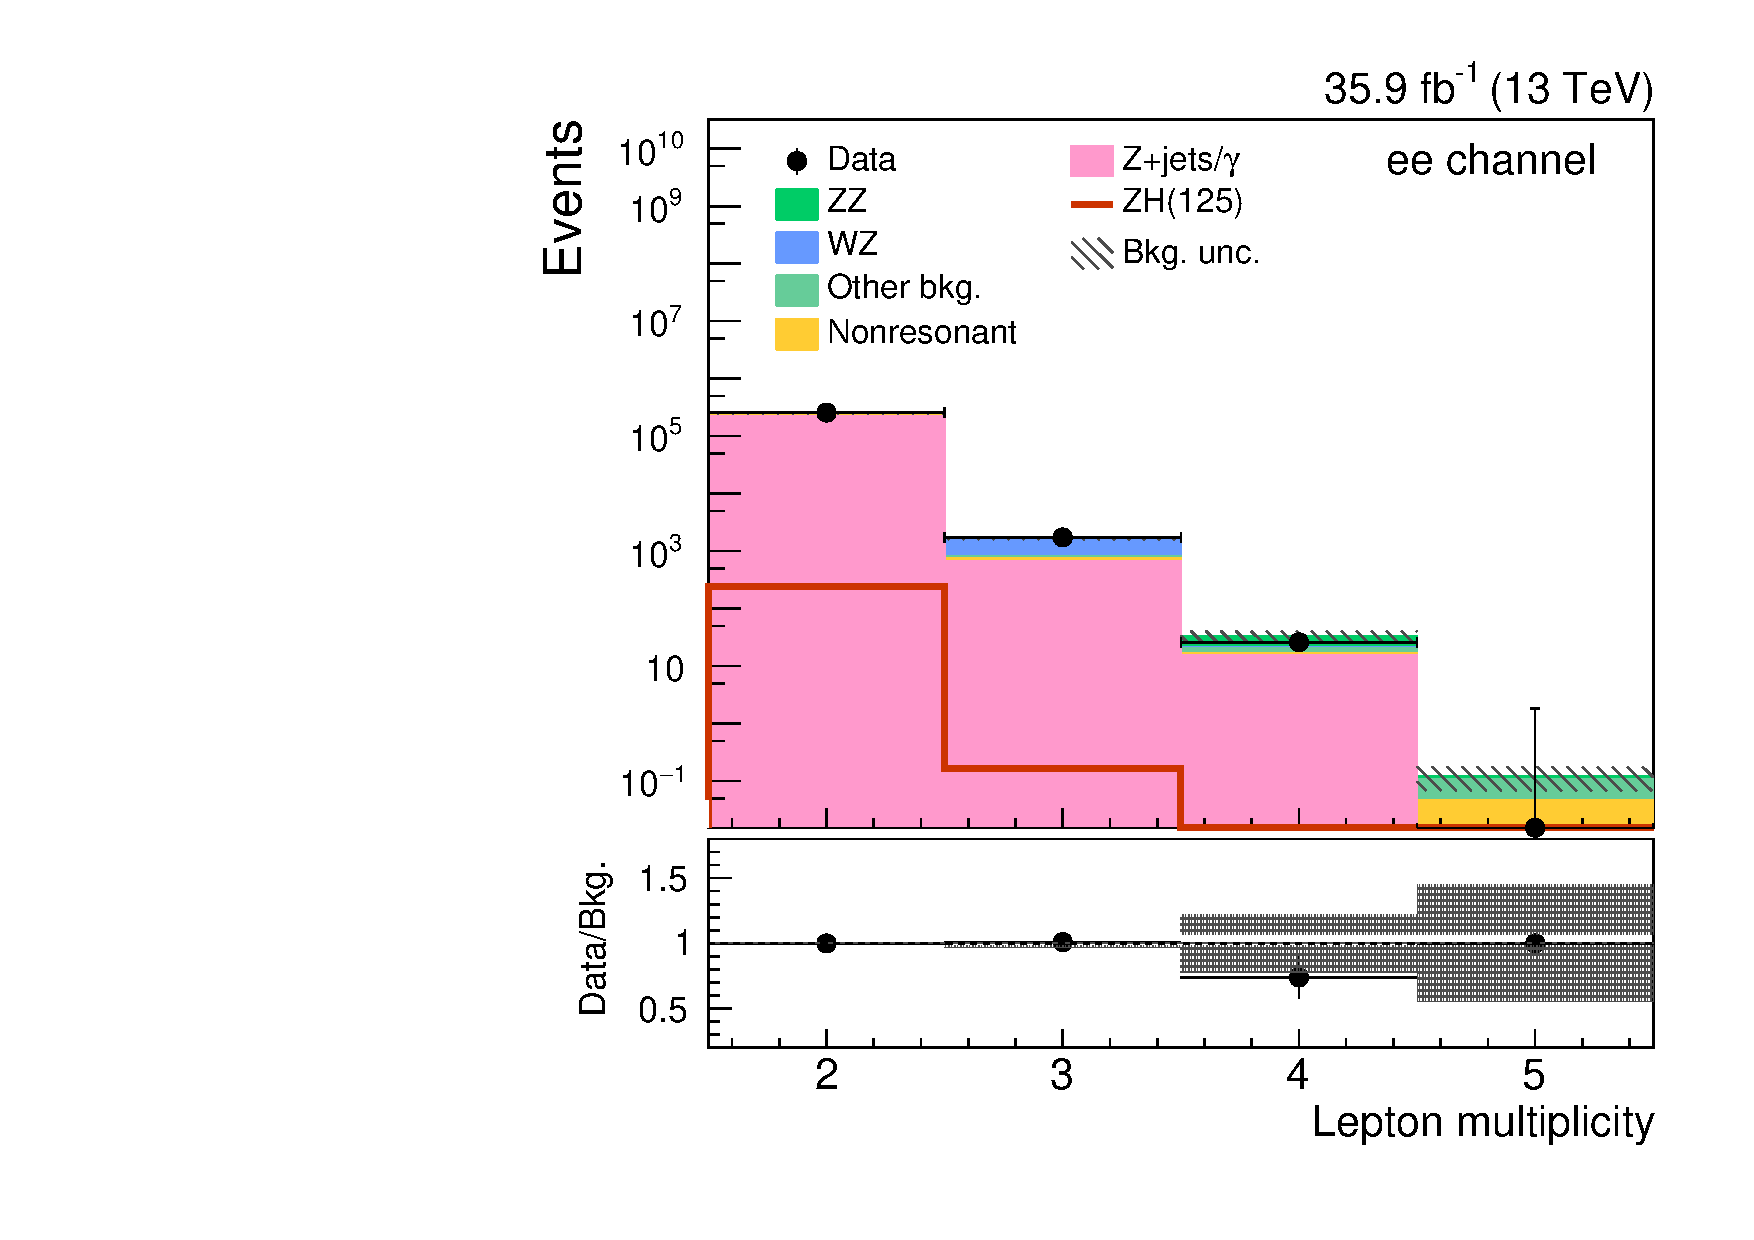
\includegraphics[width=\cmsFigWidth]{figures/zsel_nlep_ee.pdf}
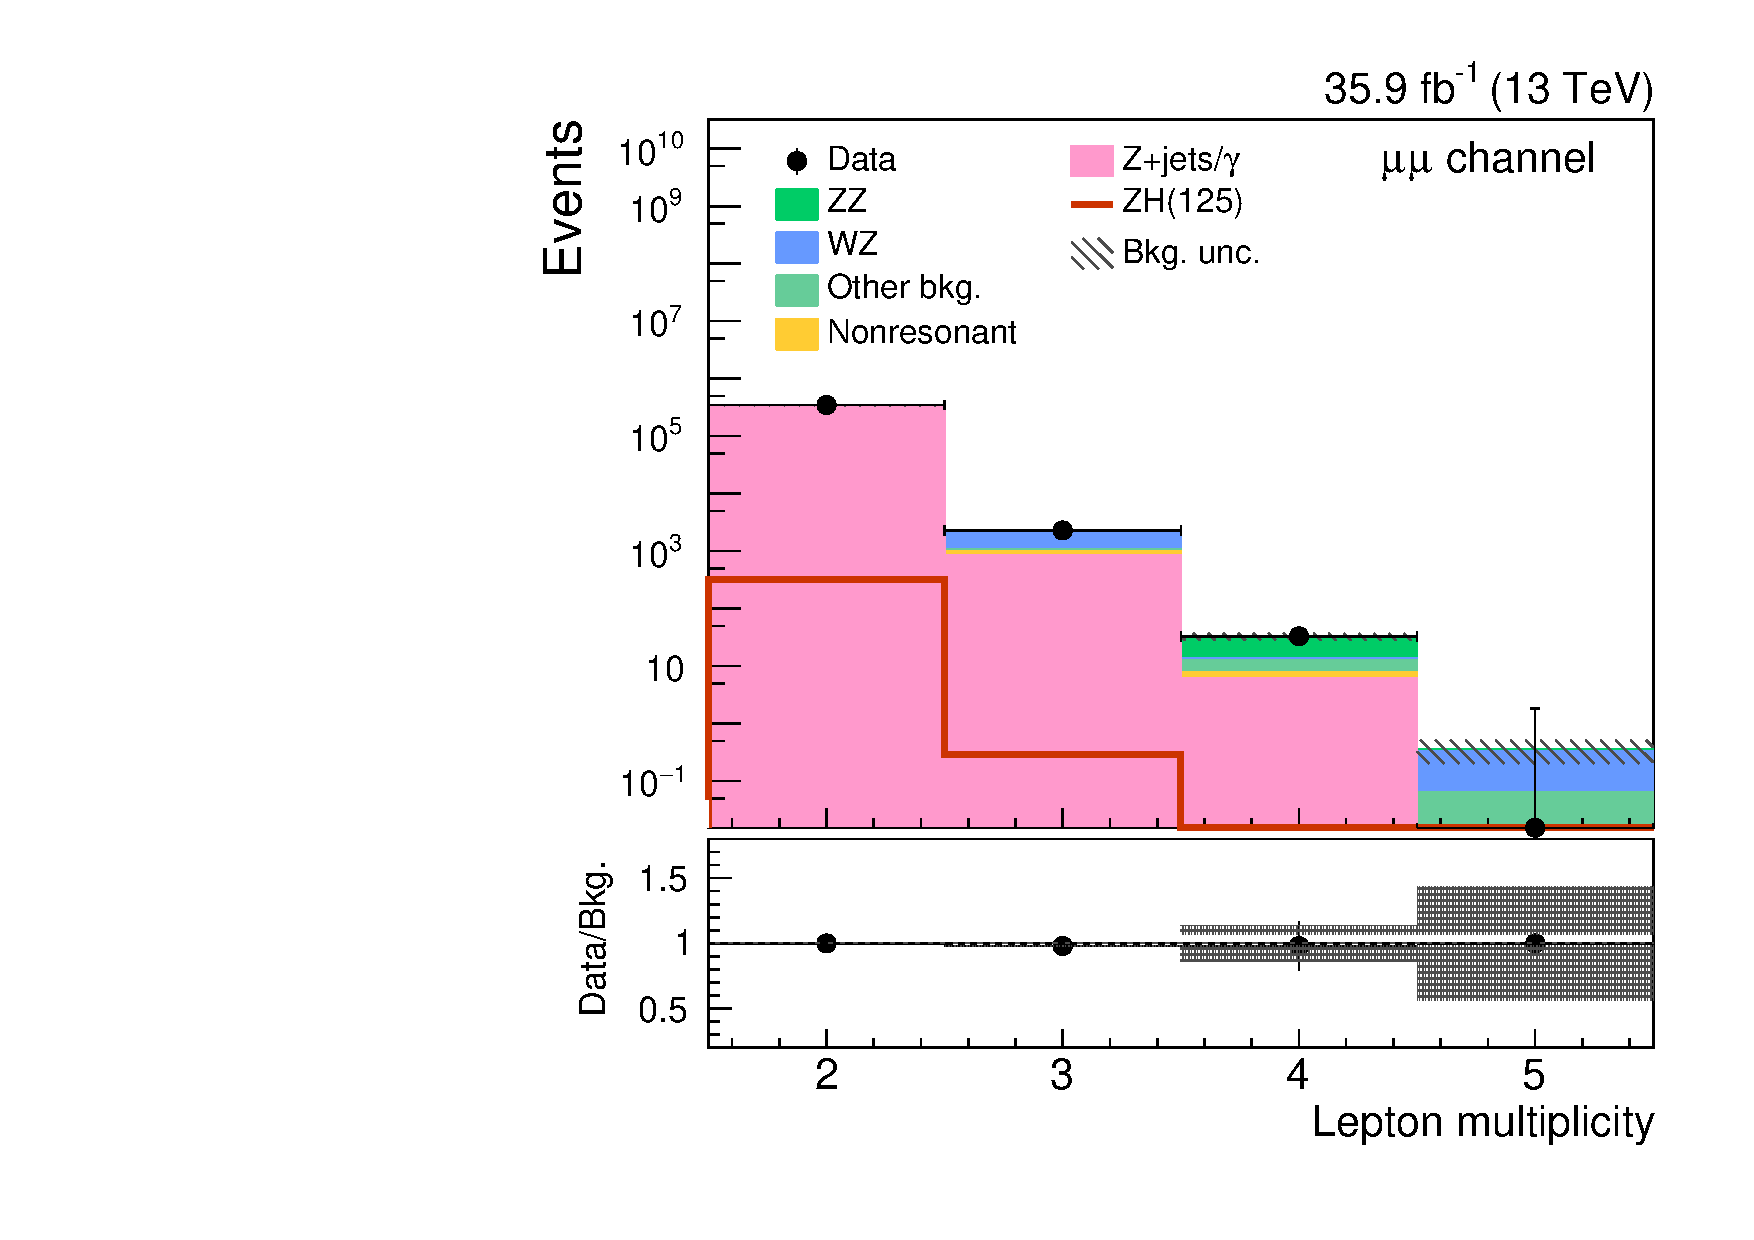
\includegraphics[width=\cmsFigWidth]{figures/zsel_nlep_mm.pdf}
\caption{
  Lepton multiplicity for each flavor channel in $\zll$ events with $\pt^{\ell\ell} > 60~\GeV$ and $\met > 40~\GeV$. 
  The uncertainty band corresponds to the statistical uncertainty only. Left: dielectron channel. Right: dimuon channel.
}
\label{fig:distributions_zsel_nlep}
\end{center}
\end{figure}
\begin{figure}[hb]
\begin{center}
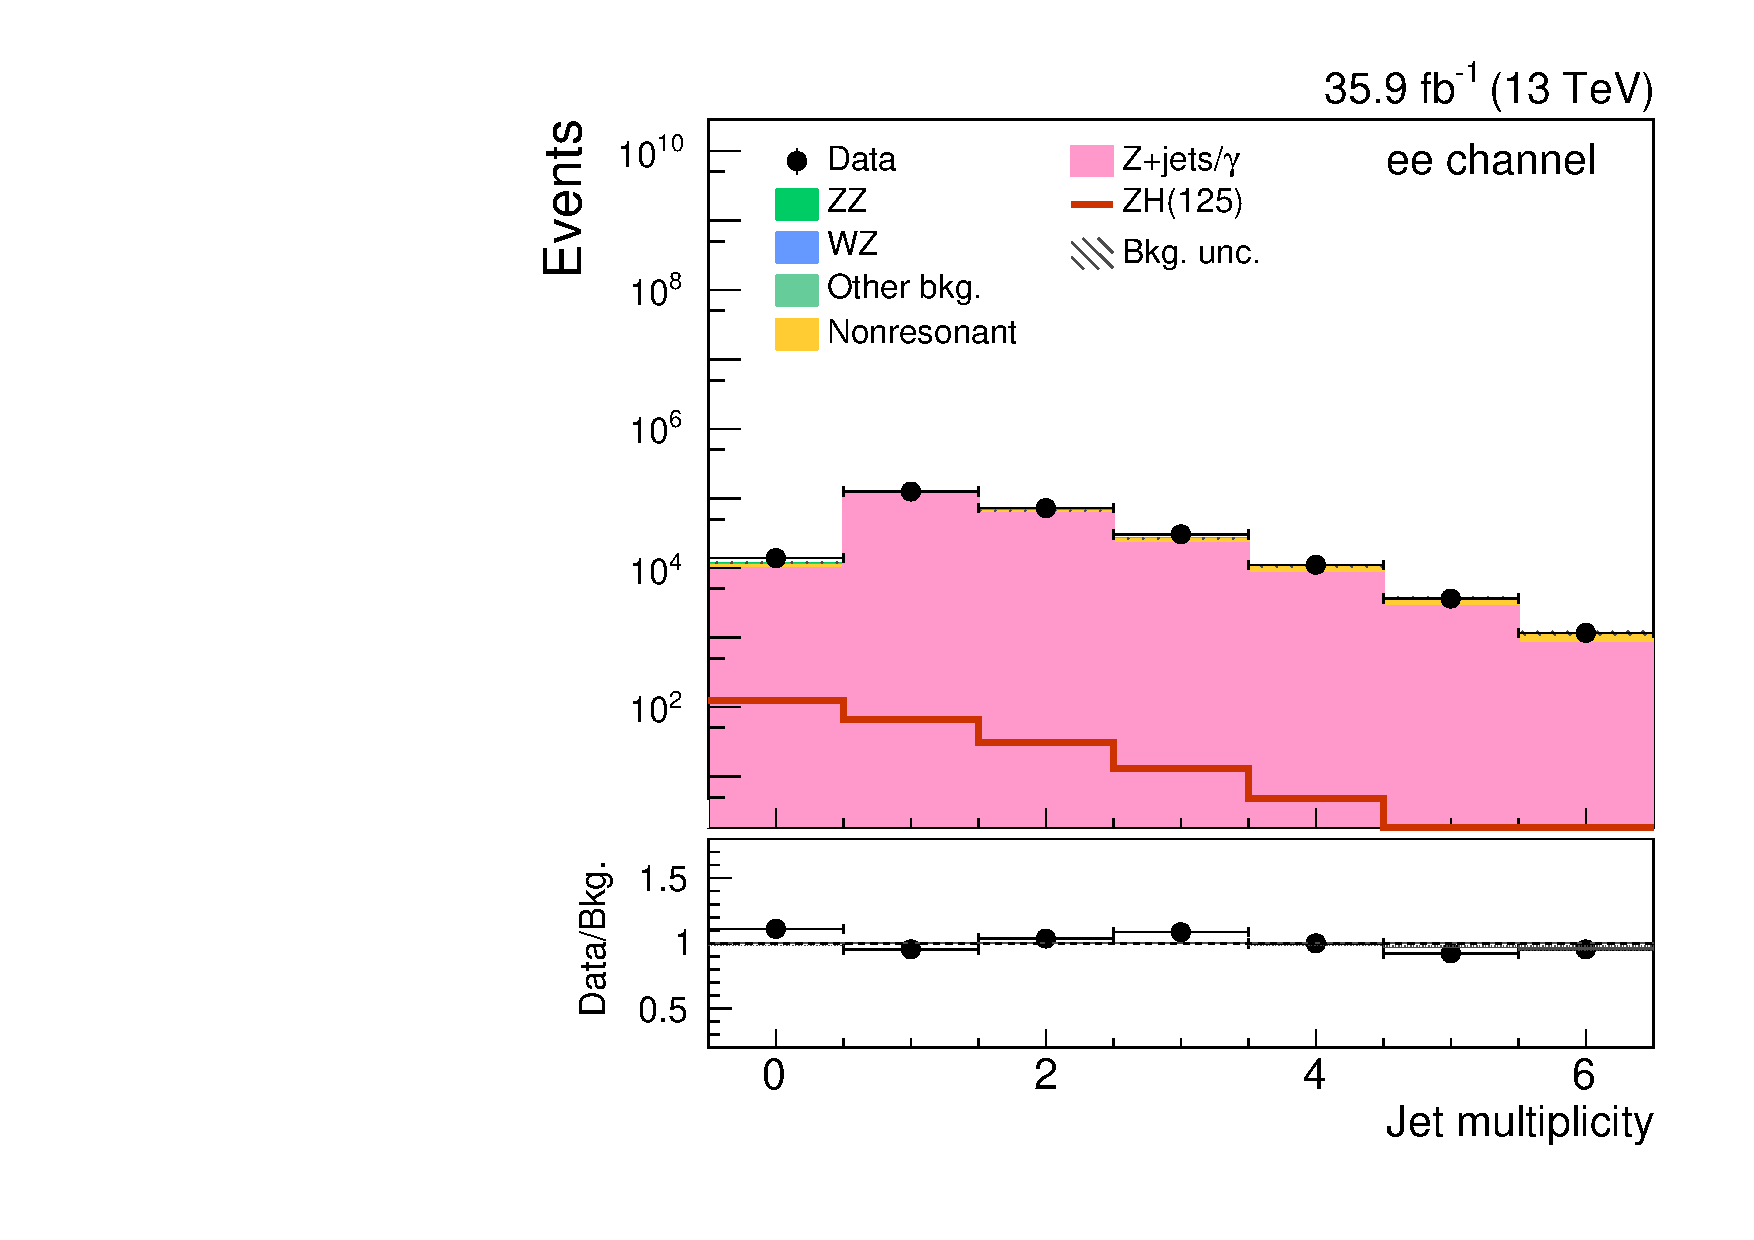
\includegraphics[width=\cmsFigWidth]{figures/zsel_njets_ee.pdf}
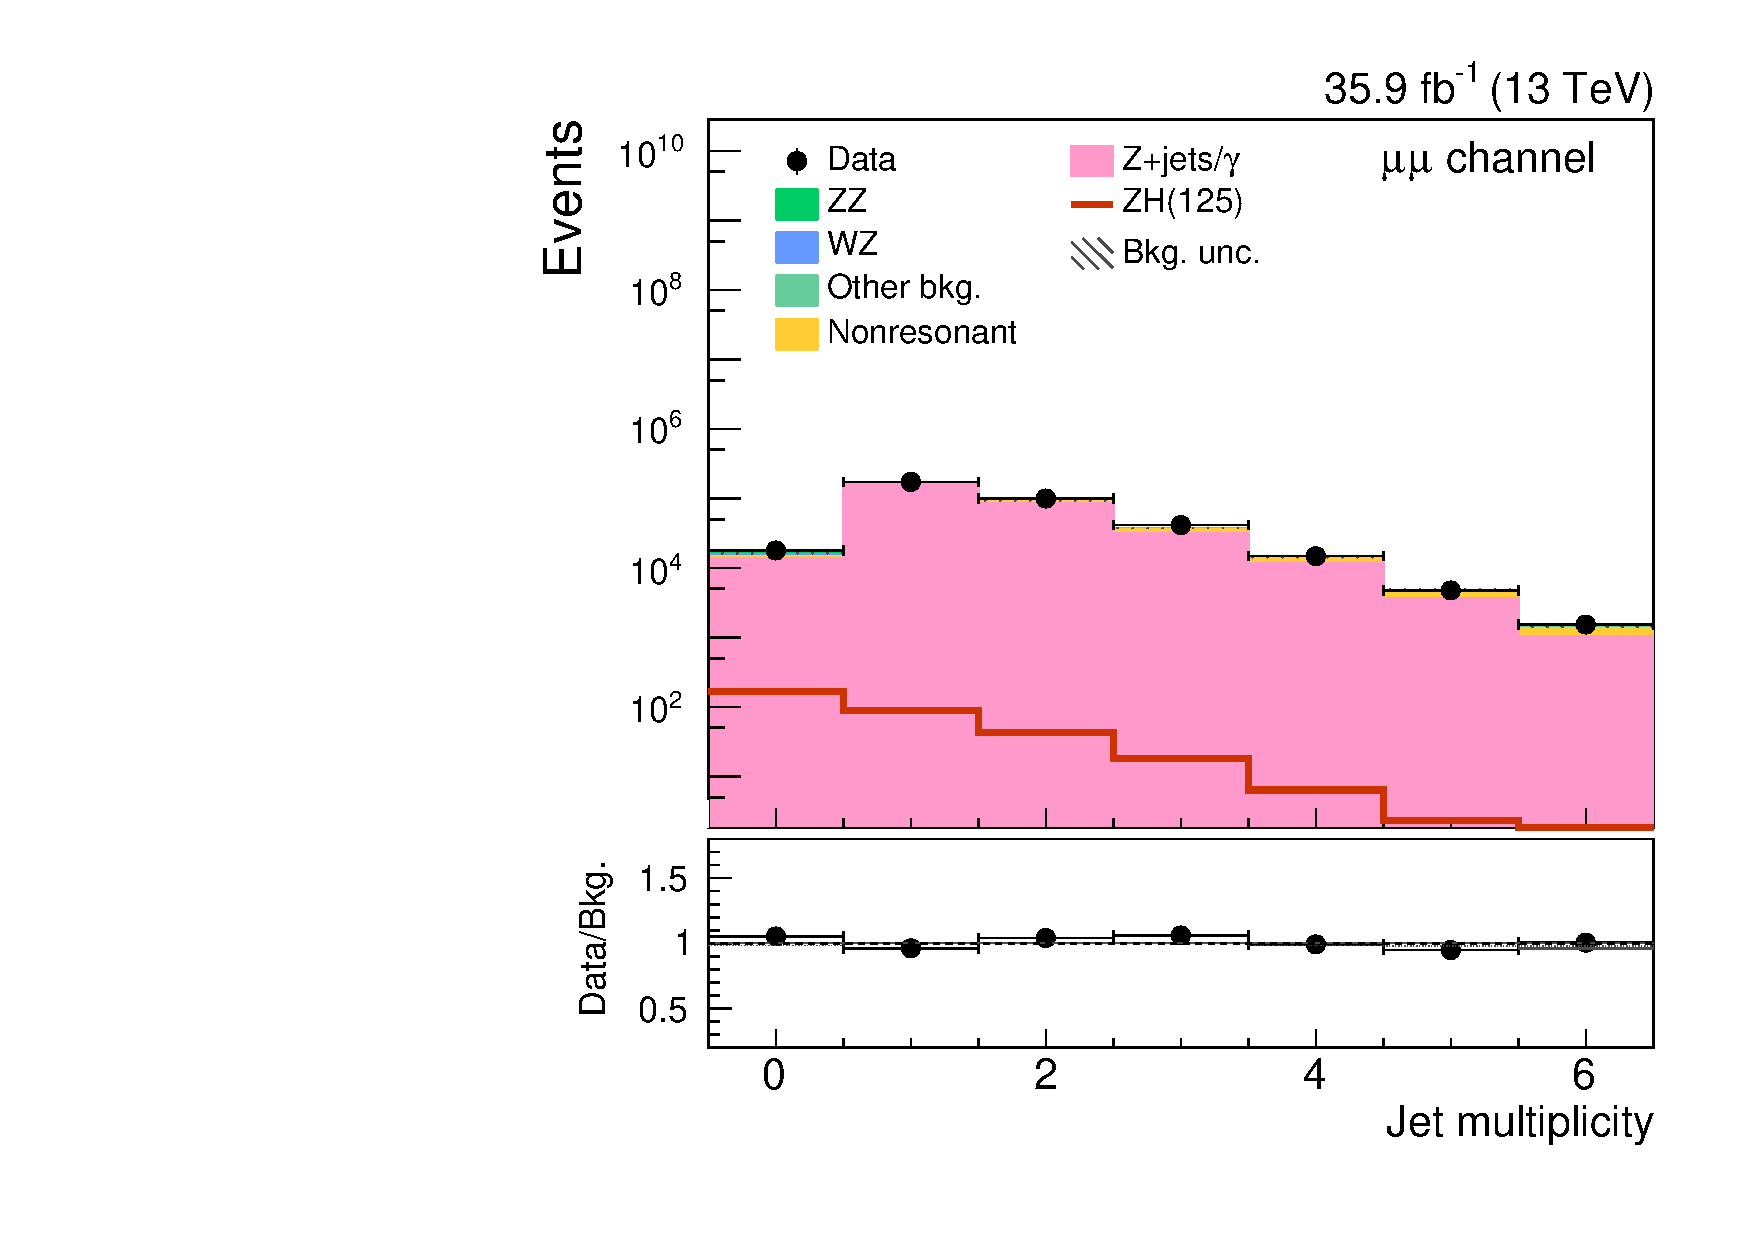
\includegraphics[width=\cmsFigWidth]{figures/zsel_njets_mm.pdf}
\caption{
  Jet multiplicity for each flavor channel in $\zll$ events with $\pt^{\ell\ell} > 60~\GeV$ and $\met > 40~\GeV$. 
  The uncertainty band corresponds to the statistical uncertainty only. Left: dielectron channel. Right: dimuon channel.
}
\label{fig:distributions_zsel_njets}
\end{center}
\end{figure}
\begin{figure}[hb]
\begin{center}
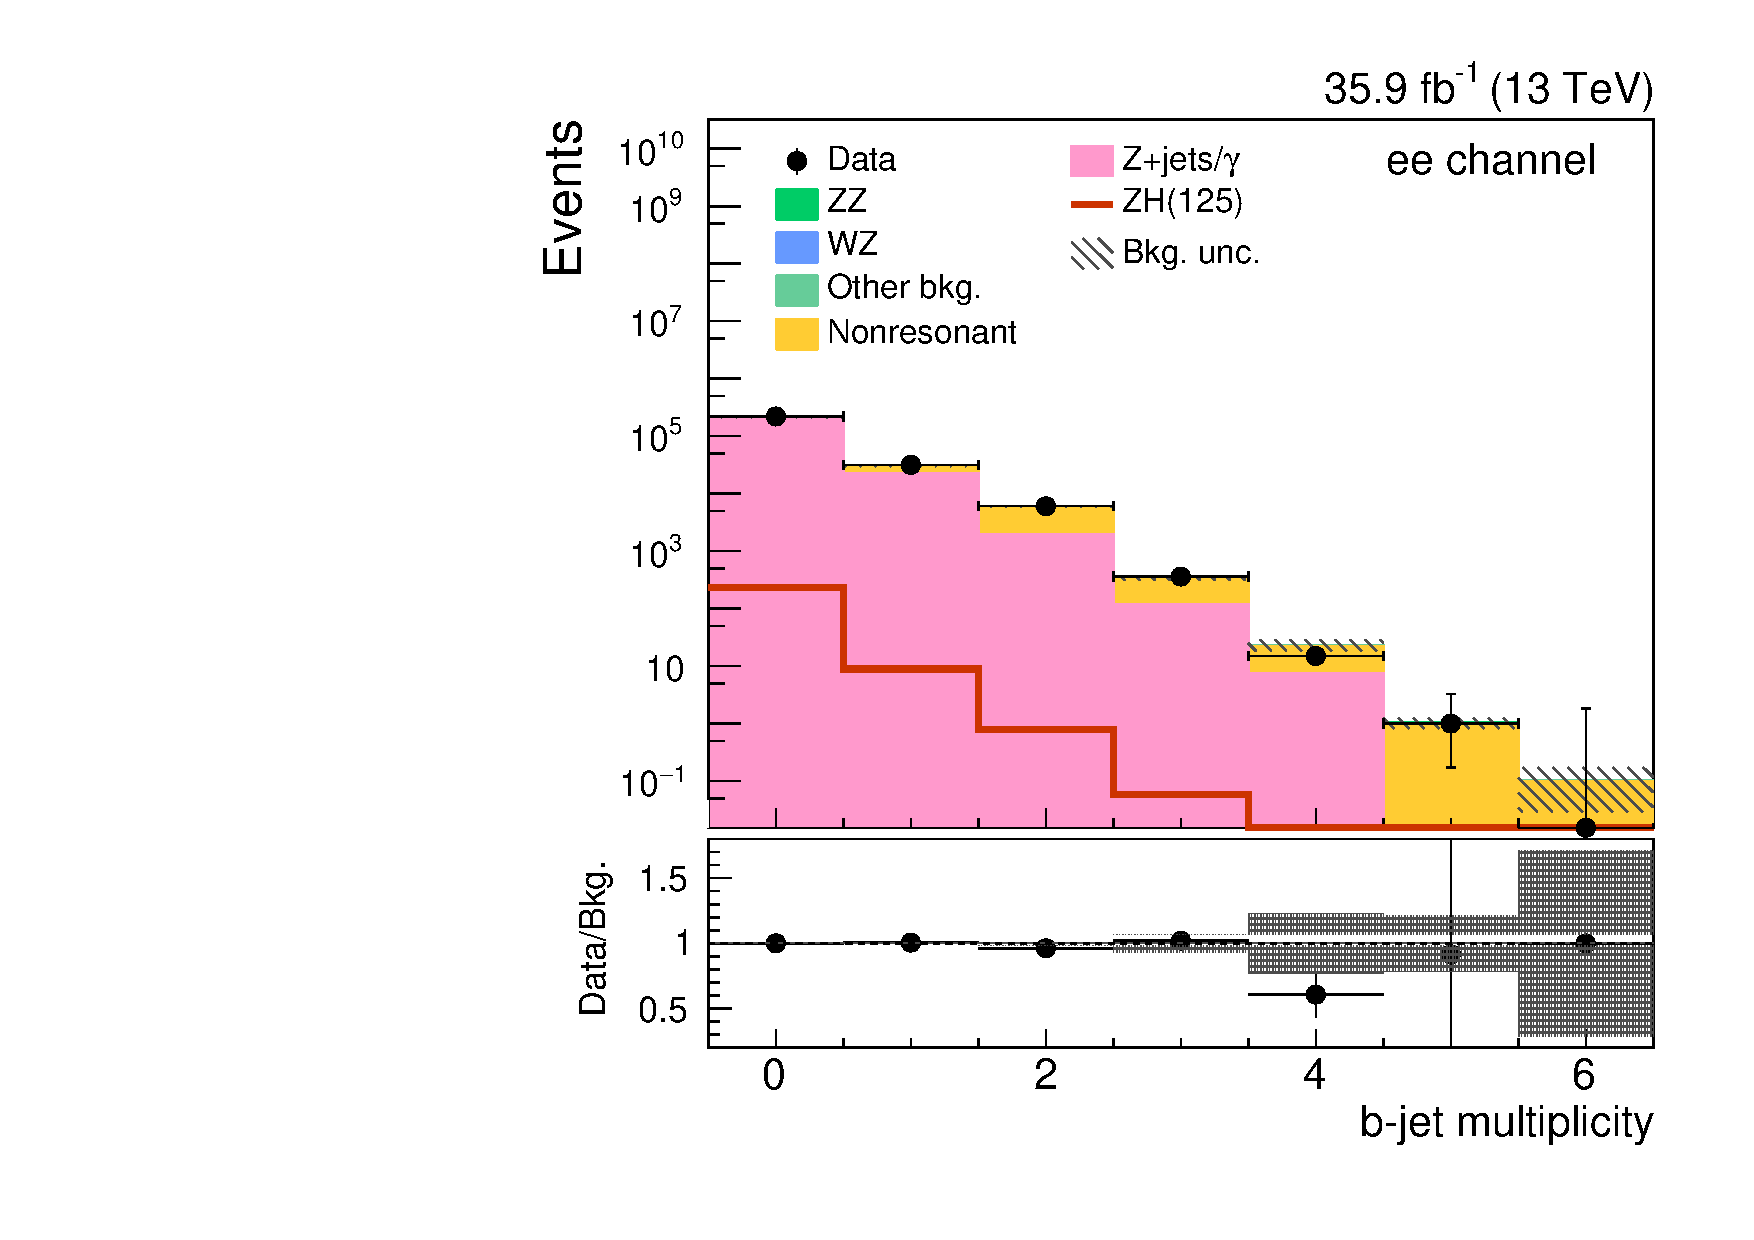
\includegraphics[width=\cmsFigWidth]{figures/zsel_bjets_ee.pdf}
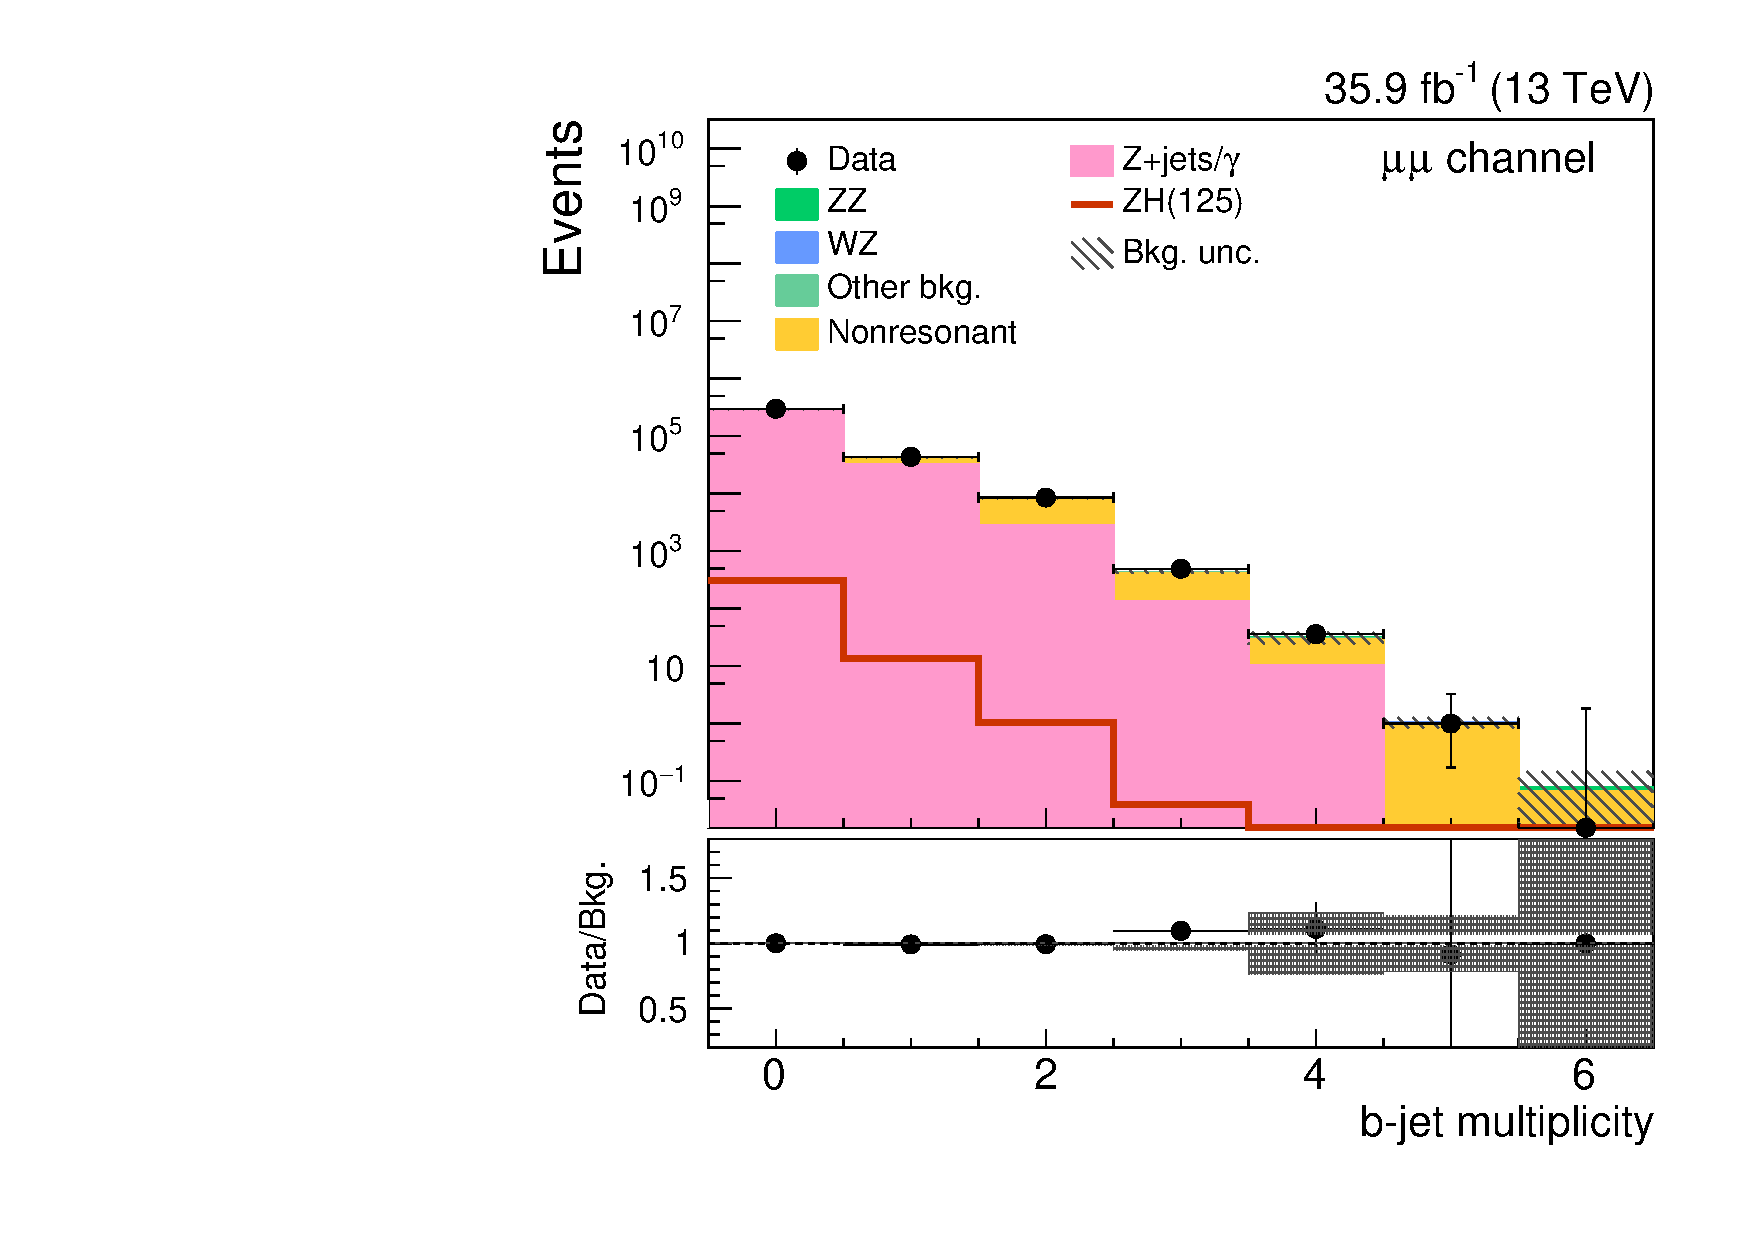
\includegraphics[width=\cmsFigWidth]{figures/zsel_bjets_mm.pdf}
\caption{
  Number of jets passing the requirements for b-tagging for each flavor channel in $\zll$ events with $\pt^{\ell\ell} > 60~\GeV$ and $\met > 40~\GeV$. 
  The uncertainty band corresponds to the statistical uncertainty only. Left: dielectron channel. Right: dimuon channel.
}
\label{fig:distributions_zsel_bjets}
\end{center}
\end{figure}
\begin{figure}[hb]
\begin{center}
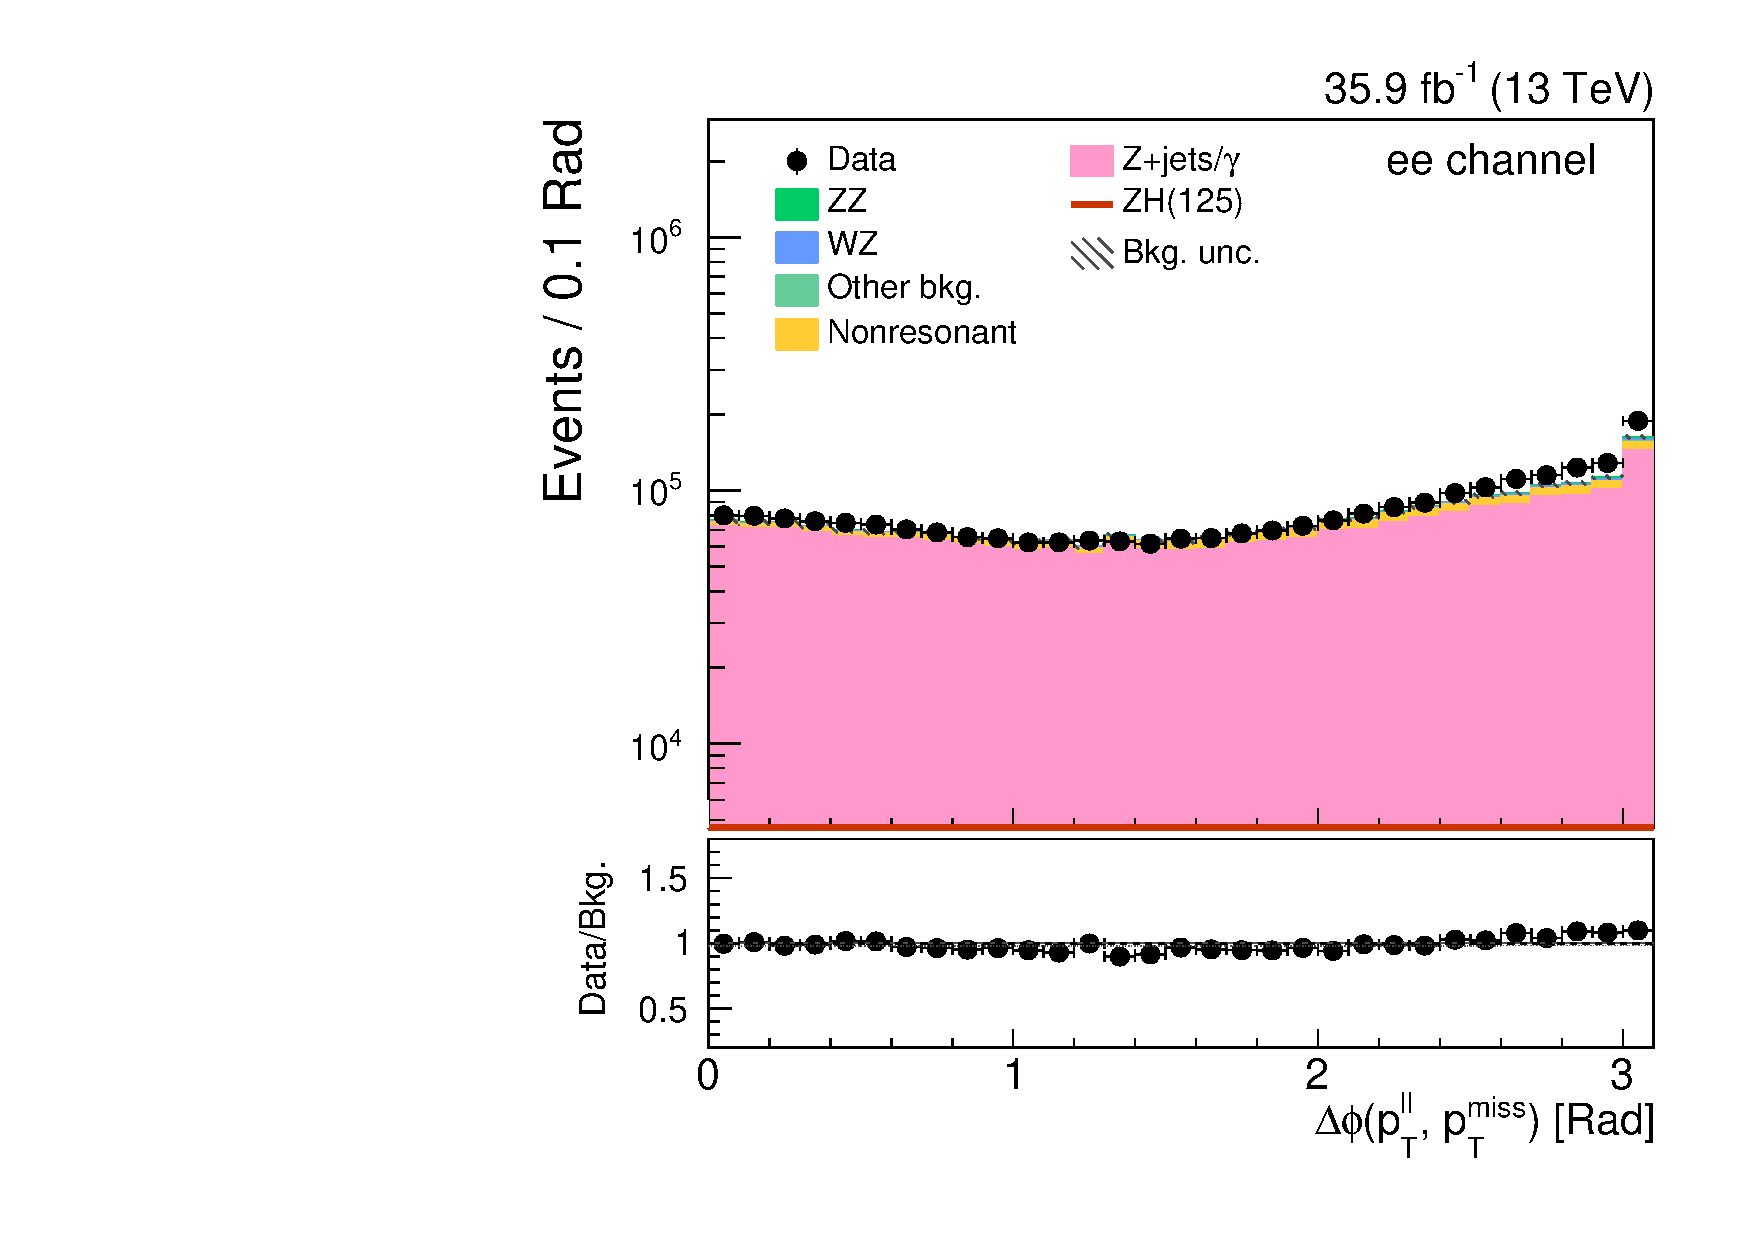
\includegraphics[width=\cmsFigWidth]{figures/zsel_dphiZMET_ee.pdf}
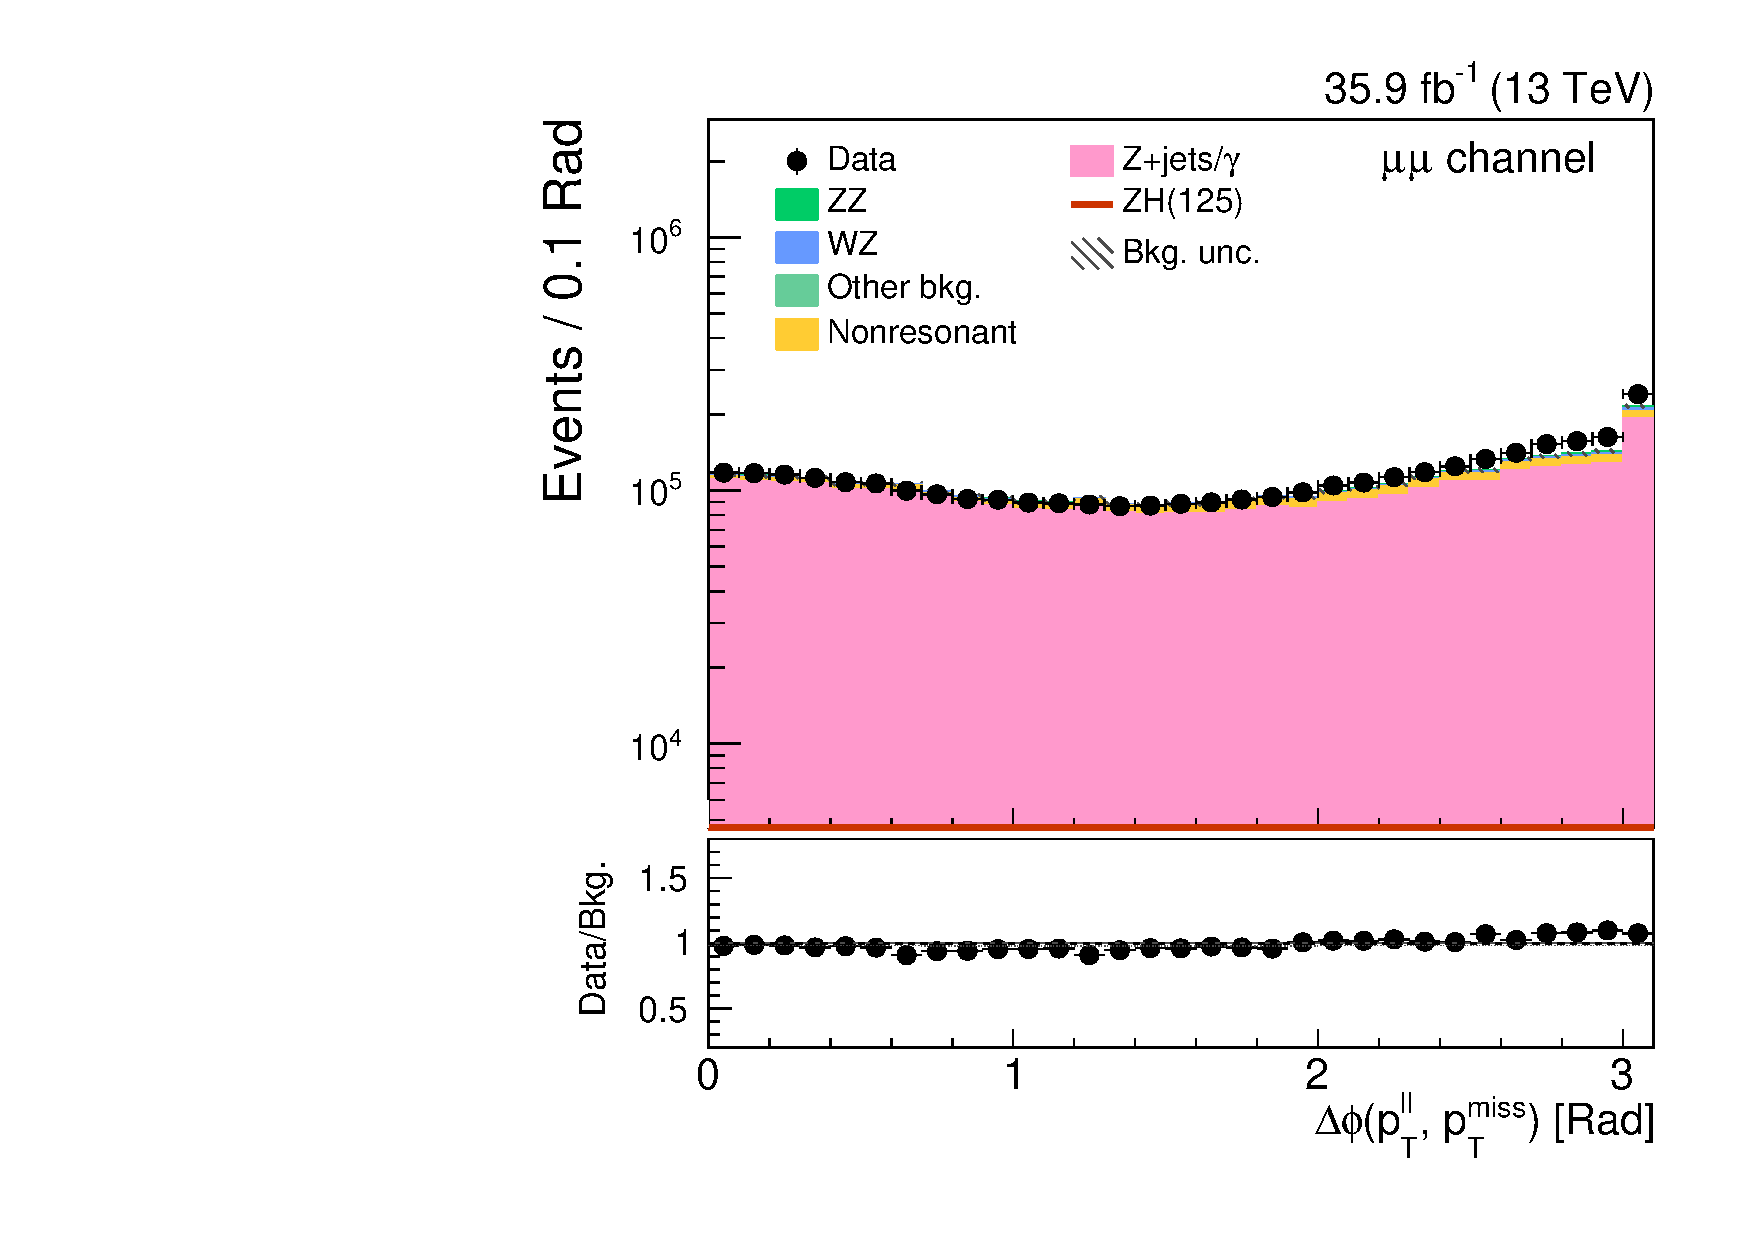
\includegraphics[width=\cmsFigWidth]{figures/zsel_dphiZMET_mm.pdf}
\caption{
  Azimuthal separation between the dilepton system and the missing transverse energy for each flavor channel in $\zll$ events with $\pt^{\ell\ell} > 60~\GeV$ and $\met > 40~\GeV$. 
  The uncertainty band corresponds to the statistical uncertainty only. Left: dielectron channel. Right: dimuon channel.
}
\label{fig:distributions_zsel_dphiZMET}
\end{center}
\end{figure}

\begin{figure}[hb]
\begin{center}
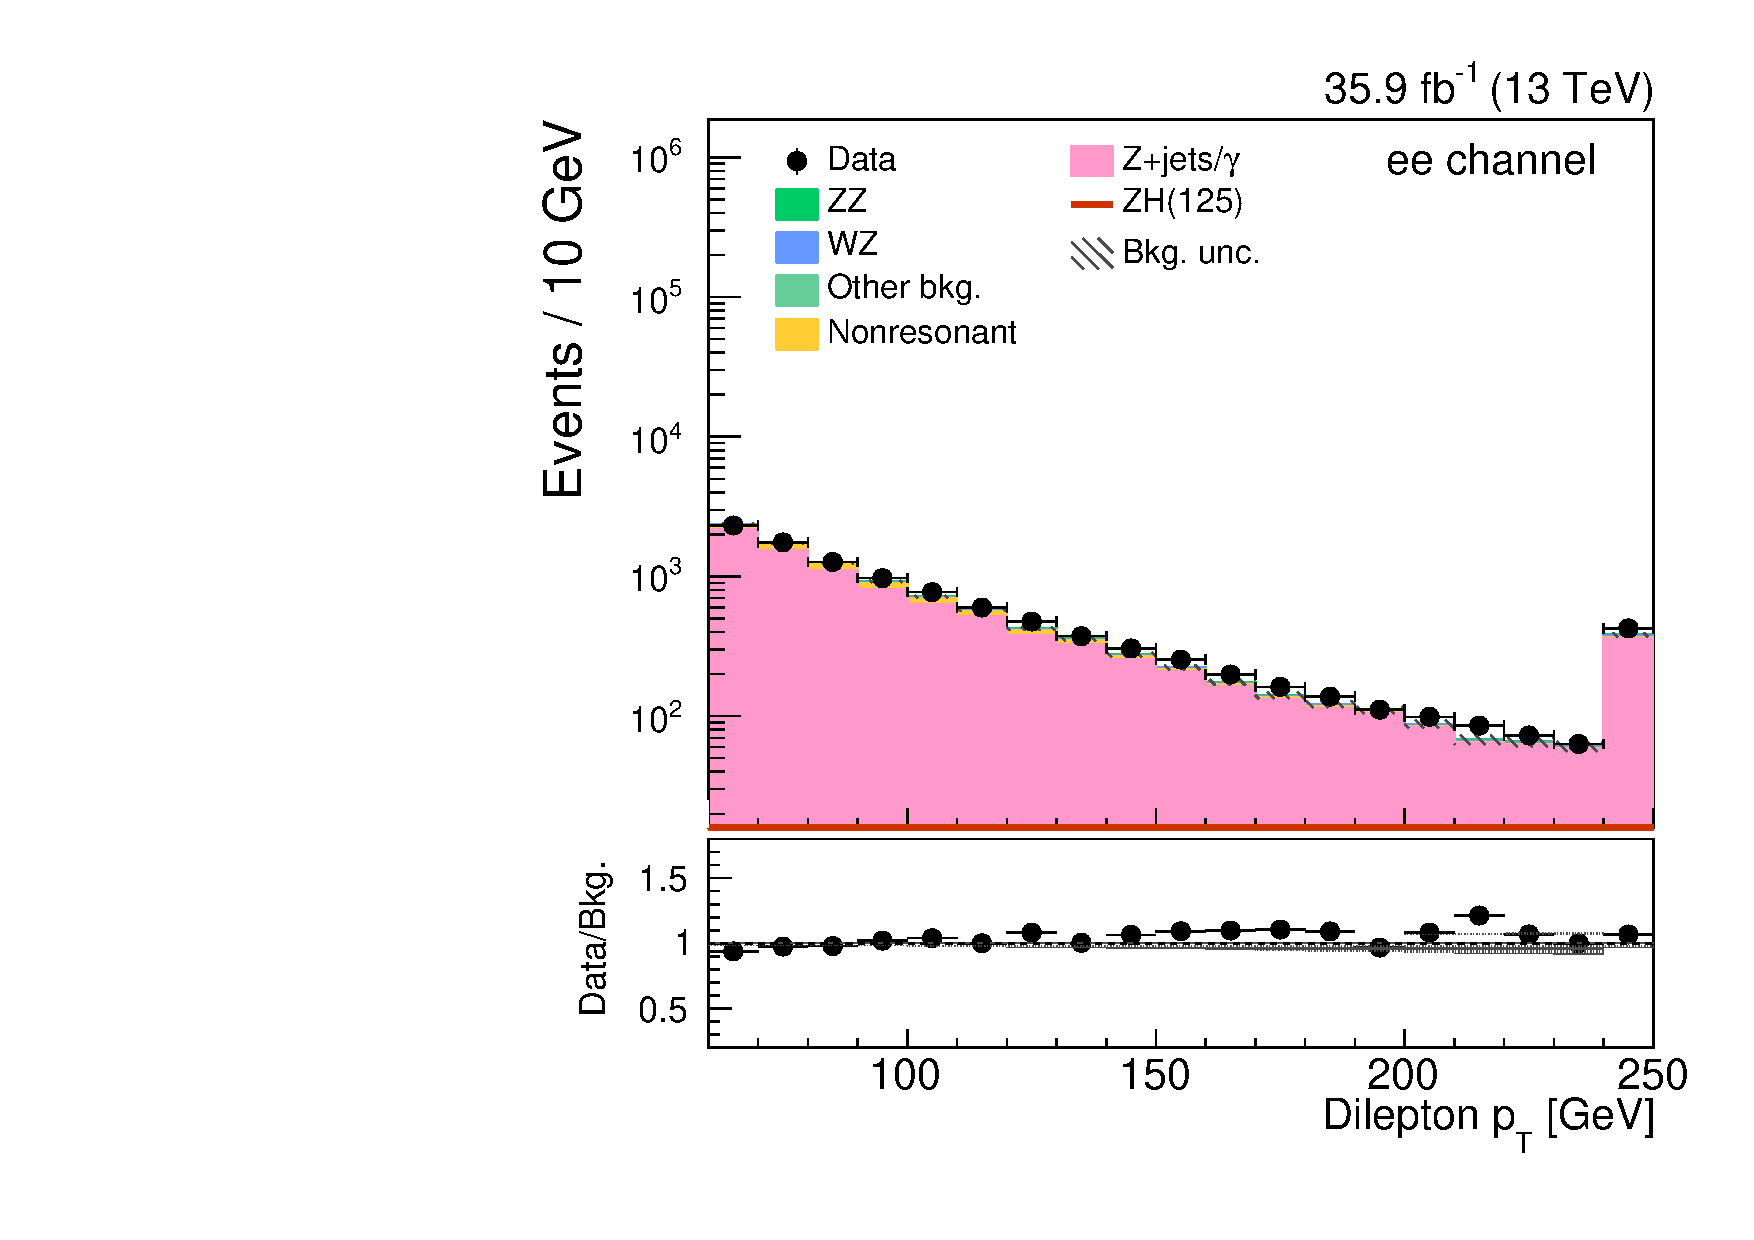
\includegraphics[width=\cmsFigWidth]{figures/presel_ptll_ee.pdf}
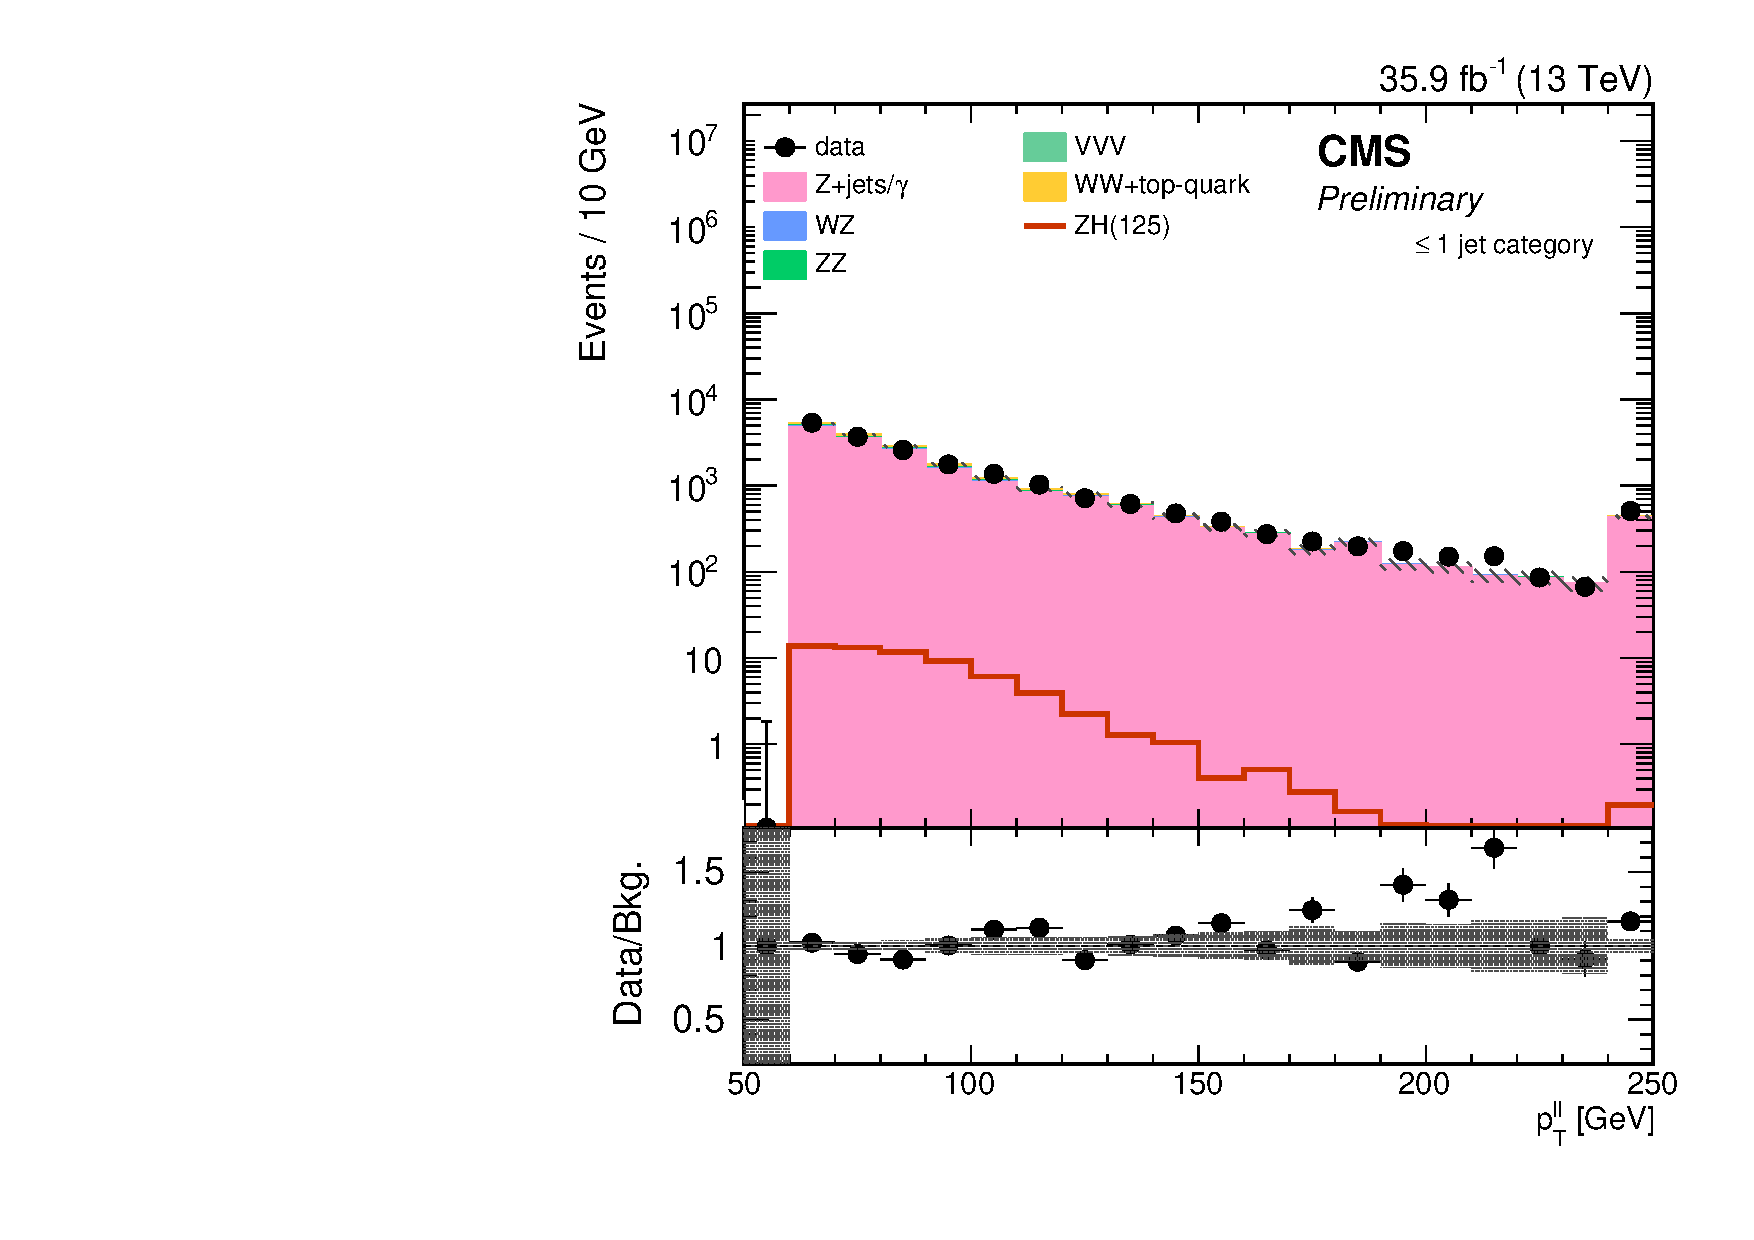
\includegraphics[width=\cmsFigWidth]{figures/presel_ptll_mm.pdf}
\caption{
  Distributions of the $\pt^{\ell\ell}$ for each flavor channel in $\zll$ events with $\pt^{\ell\ell} > 60~\GeV$ and $\met > 40~\GeV$.
  The uncertainty band corresponds to the statistical uncertainty only. Left: dielectron channel. Right: dimuon channel.
}
\label{fig:distributions_presel_ptll}
\end{center}
\end{figure}
\begin{figure}[hb]
\begin{center}
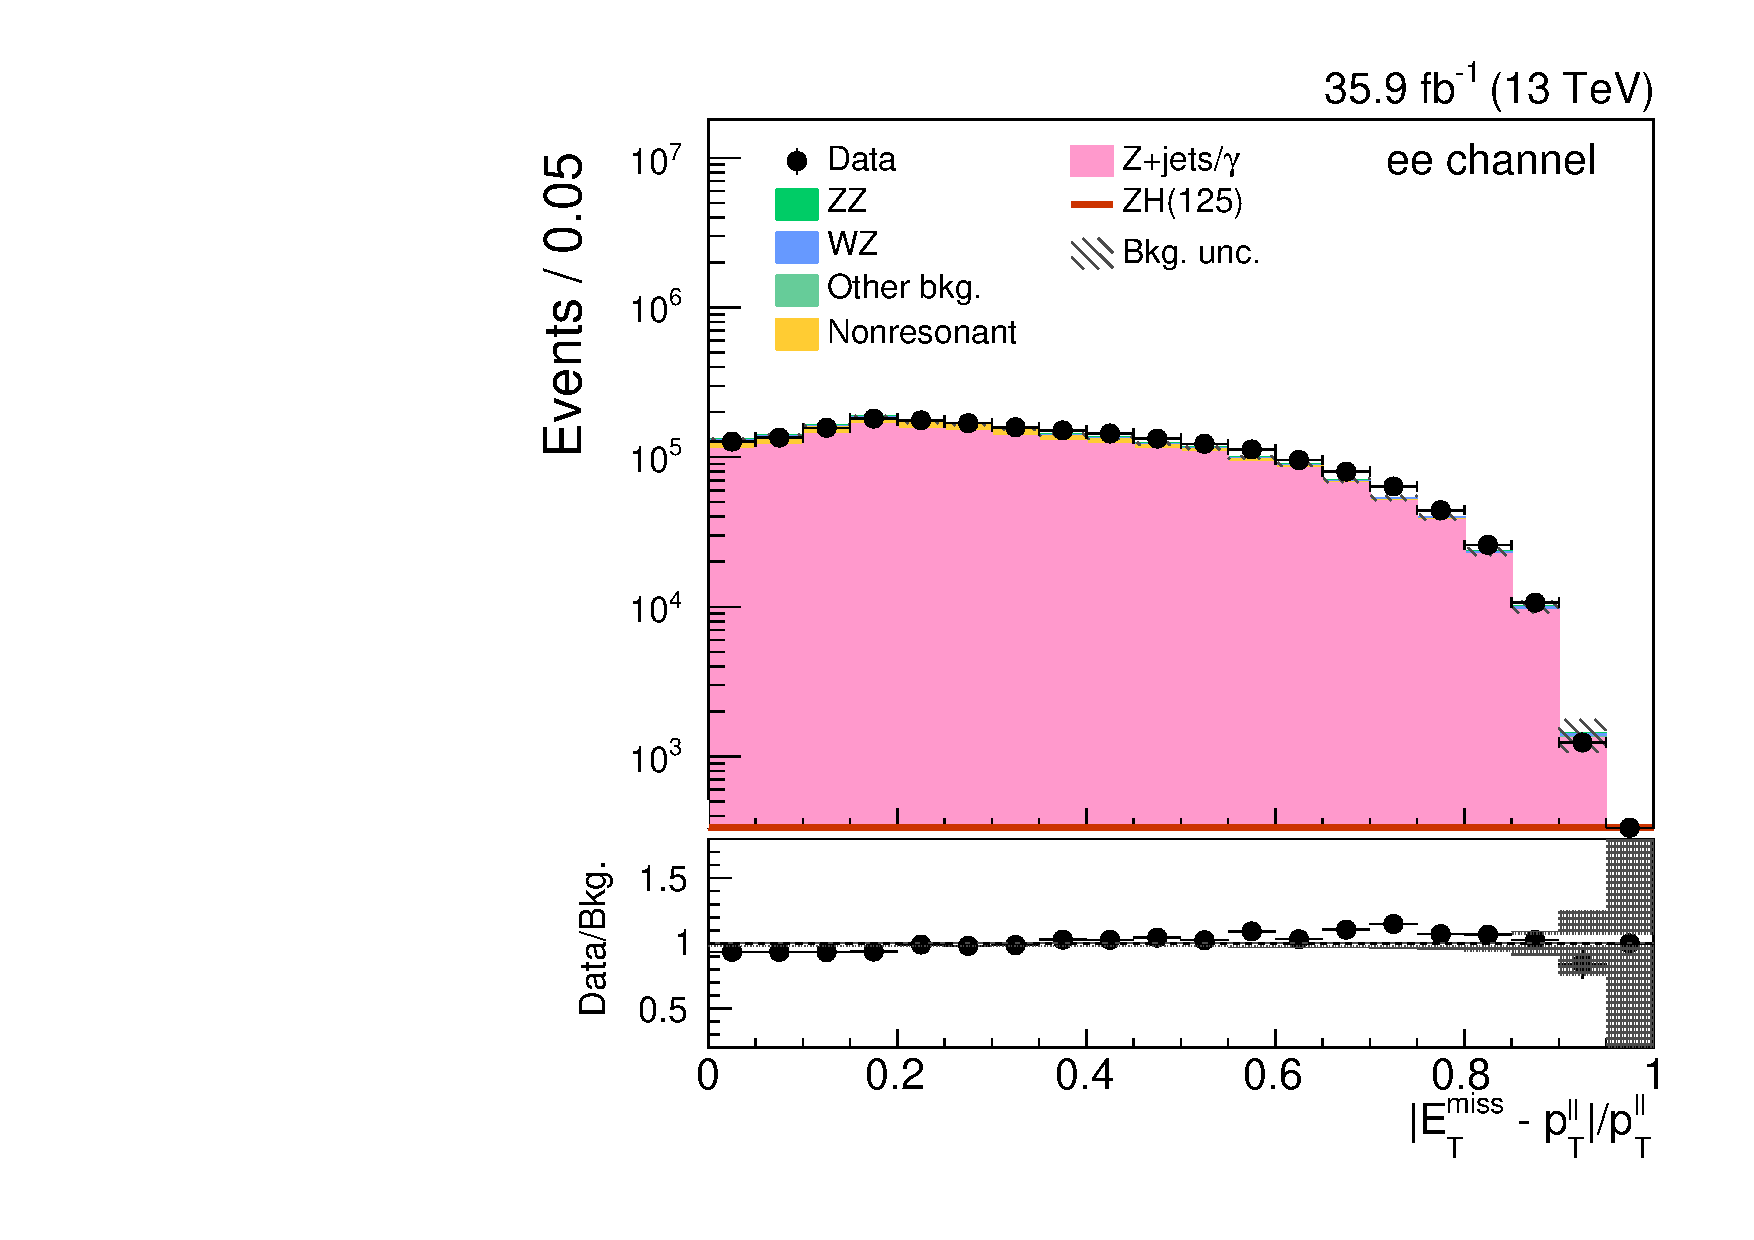
\includegraphics[width=\cmsFigWidth]{figures/presel_balance_ee.pdf}
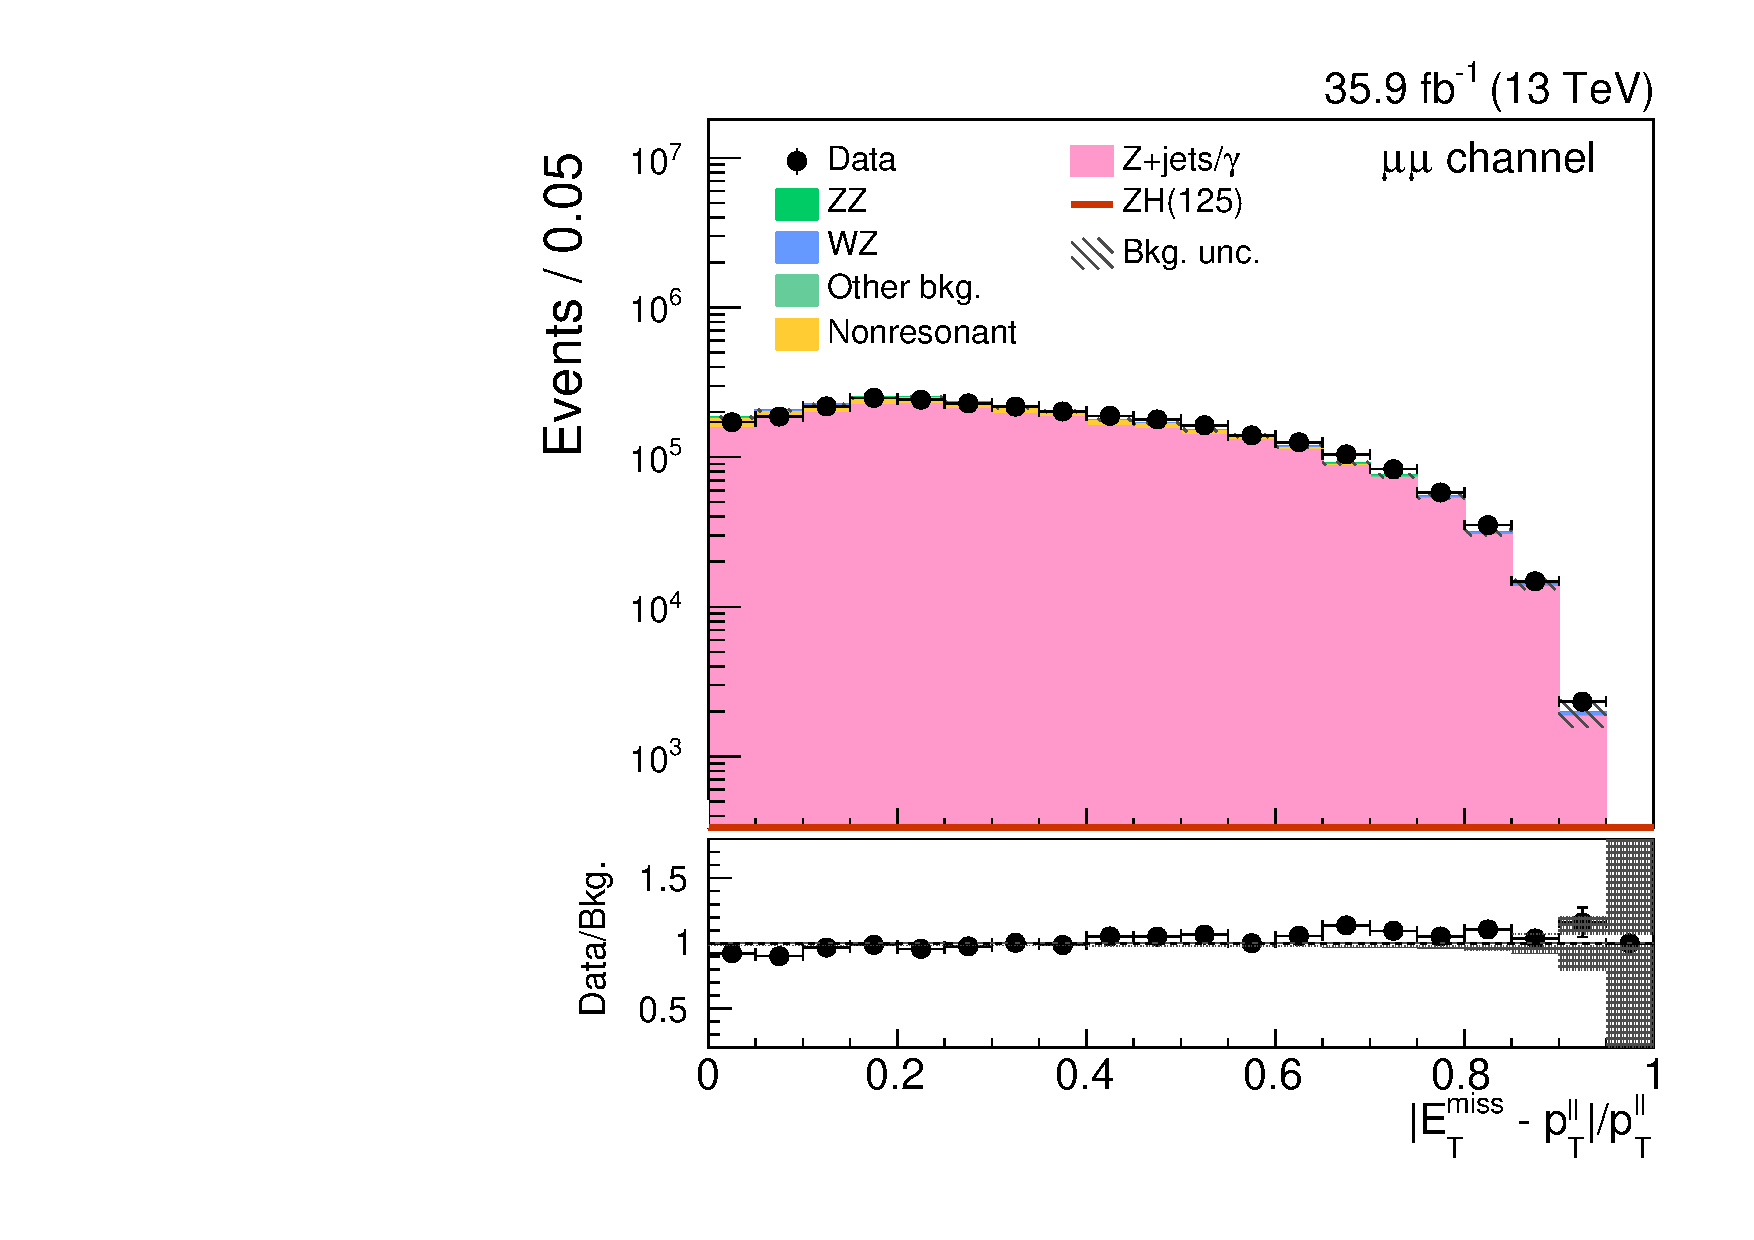
\includegraphics[width=\cmsFigWidth]{figures/presel_balance_mm.pdf}
\caption{
  Distributions of the balance variable $|\met-\pt^{\ell\ell}|/\pt^{\ell\ell}$ for each flavor channel in $\zll$ events with $\pt^{\ell\ell} > 60~\GeV$ and $\met > 40~\GeV$. 
  The uncertainty band corresponds to the statistical uncertainty only. Left: dielectron channel. Right: dimuon channel.
}
\label{fig:distributions_presel_balance}
\end{center}
\end{figure}
\begin{figure}[hb]
\begin{center}
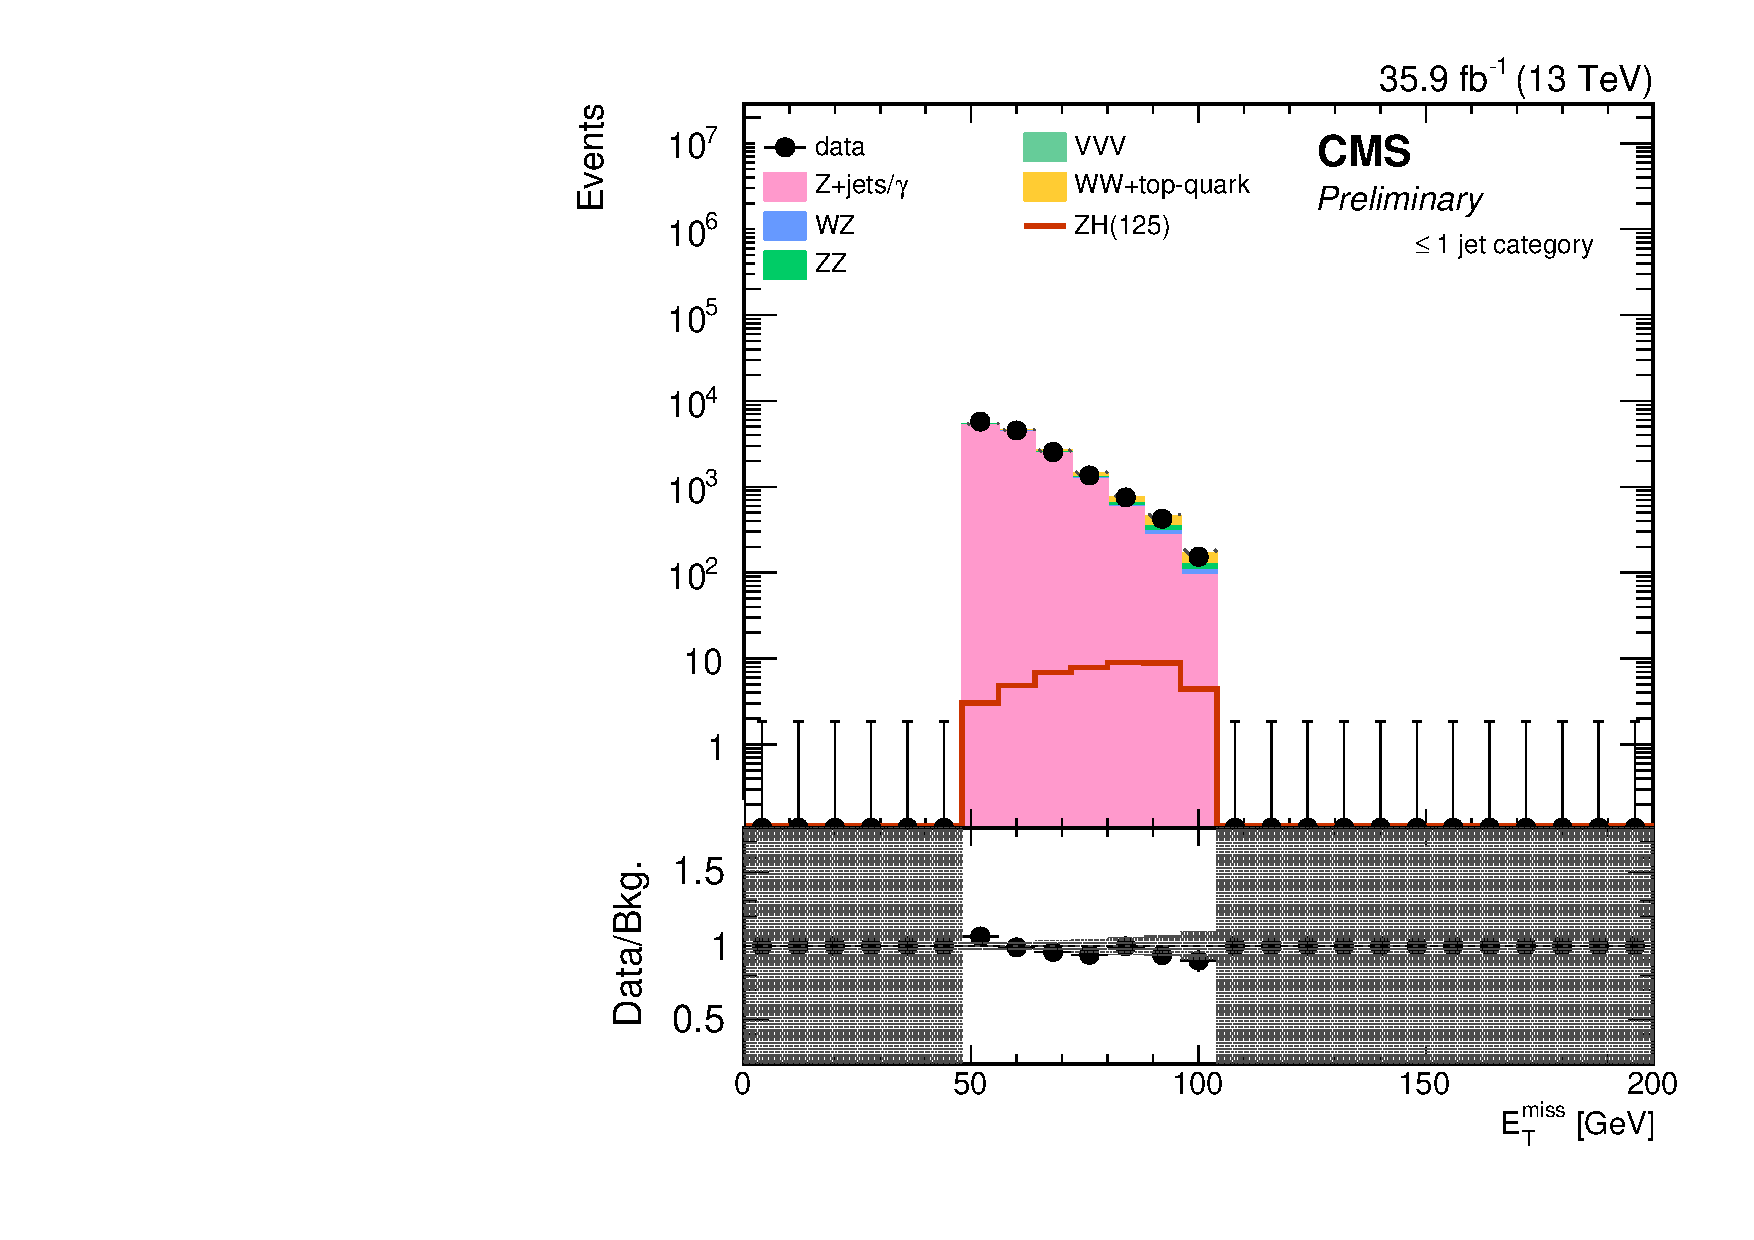
\includegraphics[width=\cmsFigWidth]{figures/presel_met_ee.pdf}
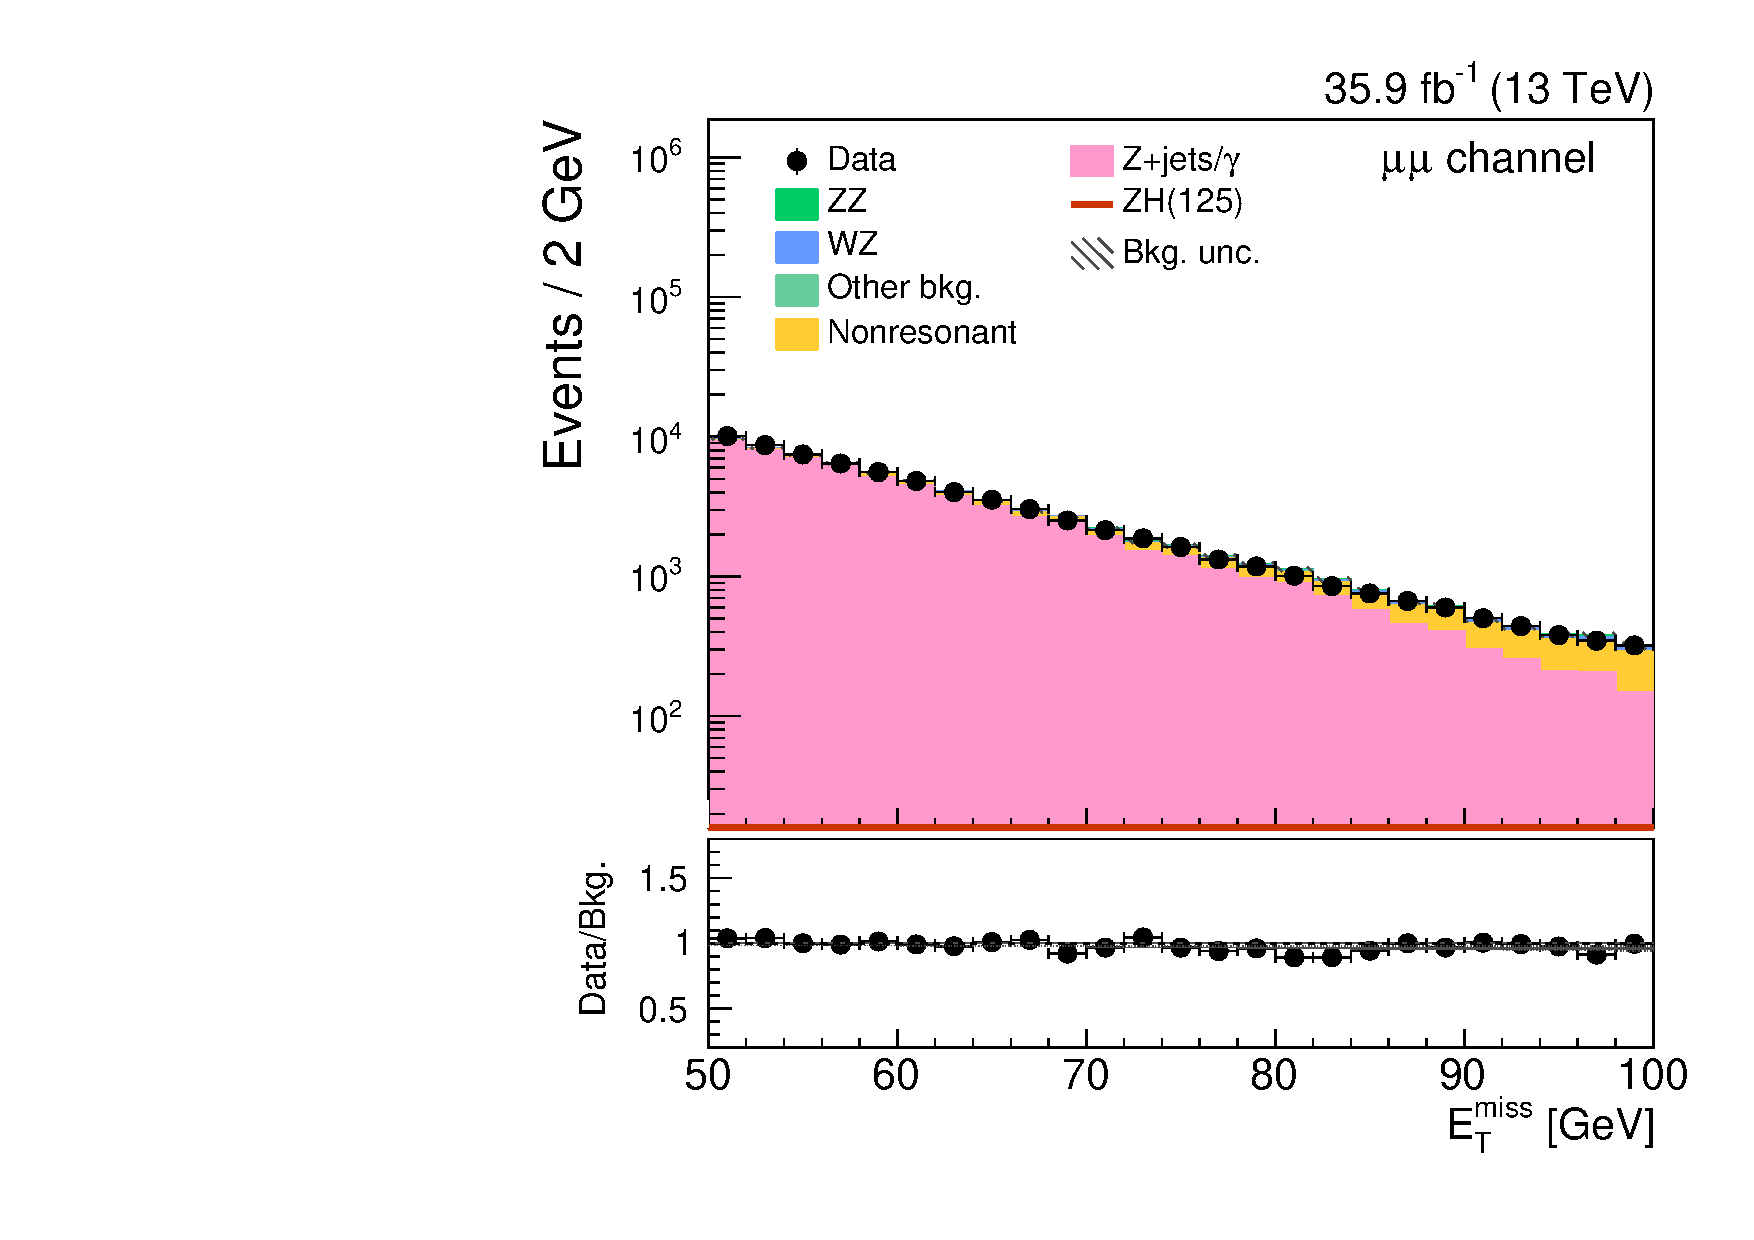
\includegraphics[width=\cmsFigWidth]{figures/presel_met_mm.pdf}
\caption{
  Distributions of the missing transverse energy for each flavor channel in $\zll$ events with $\pt^{\ell\ell} > 60~\GeV$ and $\met > 40~\GeV$.
  The uncertainty band corresponds to the statistical uncertainty only. Left: dielectron channel. Right: dimuon channel.
}
\label{fig:distributions_presel_met}
\end{center}
\end{figure}

\clearpage
\section{Background estimation}

A combination of data-driven methods and detailed simulated studies is used to
estimate background contributions.

%%%%%%%%%%%

\subsection{Diboson processes}
Contributions from the ZZ and WZ processes are estimated from control regions in data.
These processes contribute to the signal region via the
$\ZZ\rightarrow\Lep\Lep\nu\nu$ and $\WZ\rightarrow\Lep\Lep\Lep\nu$ decay modes, respectively.
In both cases, the observed $\met$ corresponds to the \pt of one of the bosons.
The processes are estimated from the control samples described in Chapter~\ref{chap:dibosons}, Sections~\ref{sec:wz3l} and~\ref{sec:zz4l}. 
The alternative decay modes allow us to probe the boson \pt distribution, which is expected to be independent of the decay mode.

%\subsubsection{\WZ control region}
%The \WZ process is estimated from events with three well-reconstructed leptons.
%In this case, the control region is populated by events from the same decay mode as the signal region, but no leptons are lost to identification and acceptance.
%A \Z candidate is selected in the same manner as for the signal region.
%An additional electron or muon fulfilling the respective POG tight ID requirement is required.
%To enhance the purity of the \WZ selection, $\met$ of at least 30\GeV is required
%the invariant mass of all three leptons $m_{3\Lep}$ is required to be larger than $100\GeV$
%and the invariant mass between all opposite sign-same flavour lepton pairs ($m_{2\Lep}$) is required to be larger than $4\GeV$.
%These requirements follow the procedure used in the CMS measurement of the \WZ production cross-section~\cite{smp16002}.
%
%The \W boson $\pt$ (``emulated \met'') is estimated by calculating the vectorial sum of the $\met$ vector and the transverse momentum vector of the third lepton.
%Using the emulated \met and the dilepton candidate, the same topological selection is applied as for the signal region.
%Since there is no danger of contamination, no veto on additional $\tau$ leptons is applied, and the b jet veto is relaxed to only reject events where a jet passes the tight working point of the b jet ID.
%
%The resulting emulated \met spectrum is shown in fig.~\ref{fig:histo_fakemet} (left).
%
%\subsubsection{\ZZ control region}
%The \ZZ process is estimated from events with four well-reconstructed leptons.
%In addition to a signal-like \Z candidate, a second candidate is required, the constituents of which only need to pass loose ID requirement.
%This choice reflects the very high purity of the four-lepton selection. For both candidates, a signal-like \Z mass requirement is enforced.
%
%Similar to the \WZ case, the emulated \met is calculated as the vectorial sum of the real \met and the \Z boson with the larger mass difference to the nominal value of $m_Z$
%\footnote{The choice of which \Z candidate to use for the emulated \MET estimate has been shown to cause very little difference in the resulting distribution.}.
%Again, a signal-like topology selection is applied using the emulated \met and the remaining \Z candidate with relaxed $\tau$ and b jet vetoes.
%
%The resulting emulated \met spectrum is shown in fig.~\ref{fig:histo_fakemet} (right).


%\begin{figure}[hb]
%\centering
%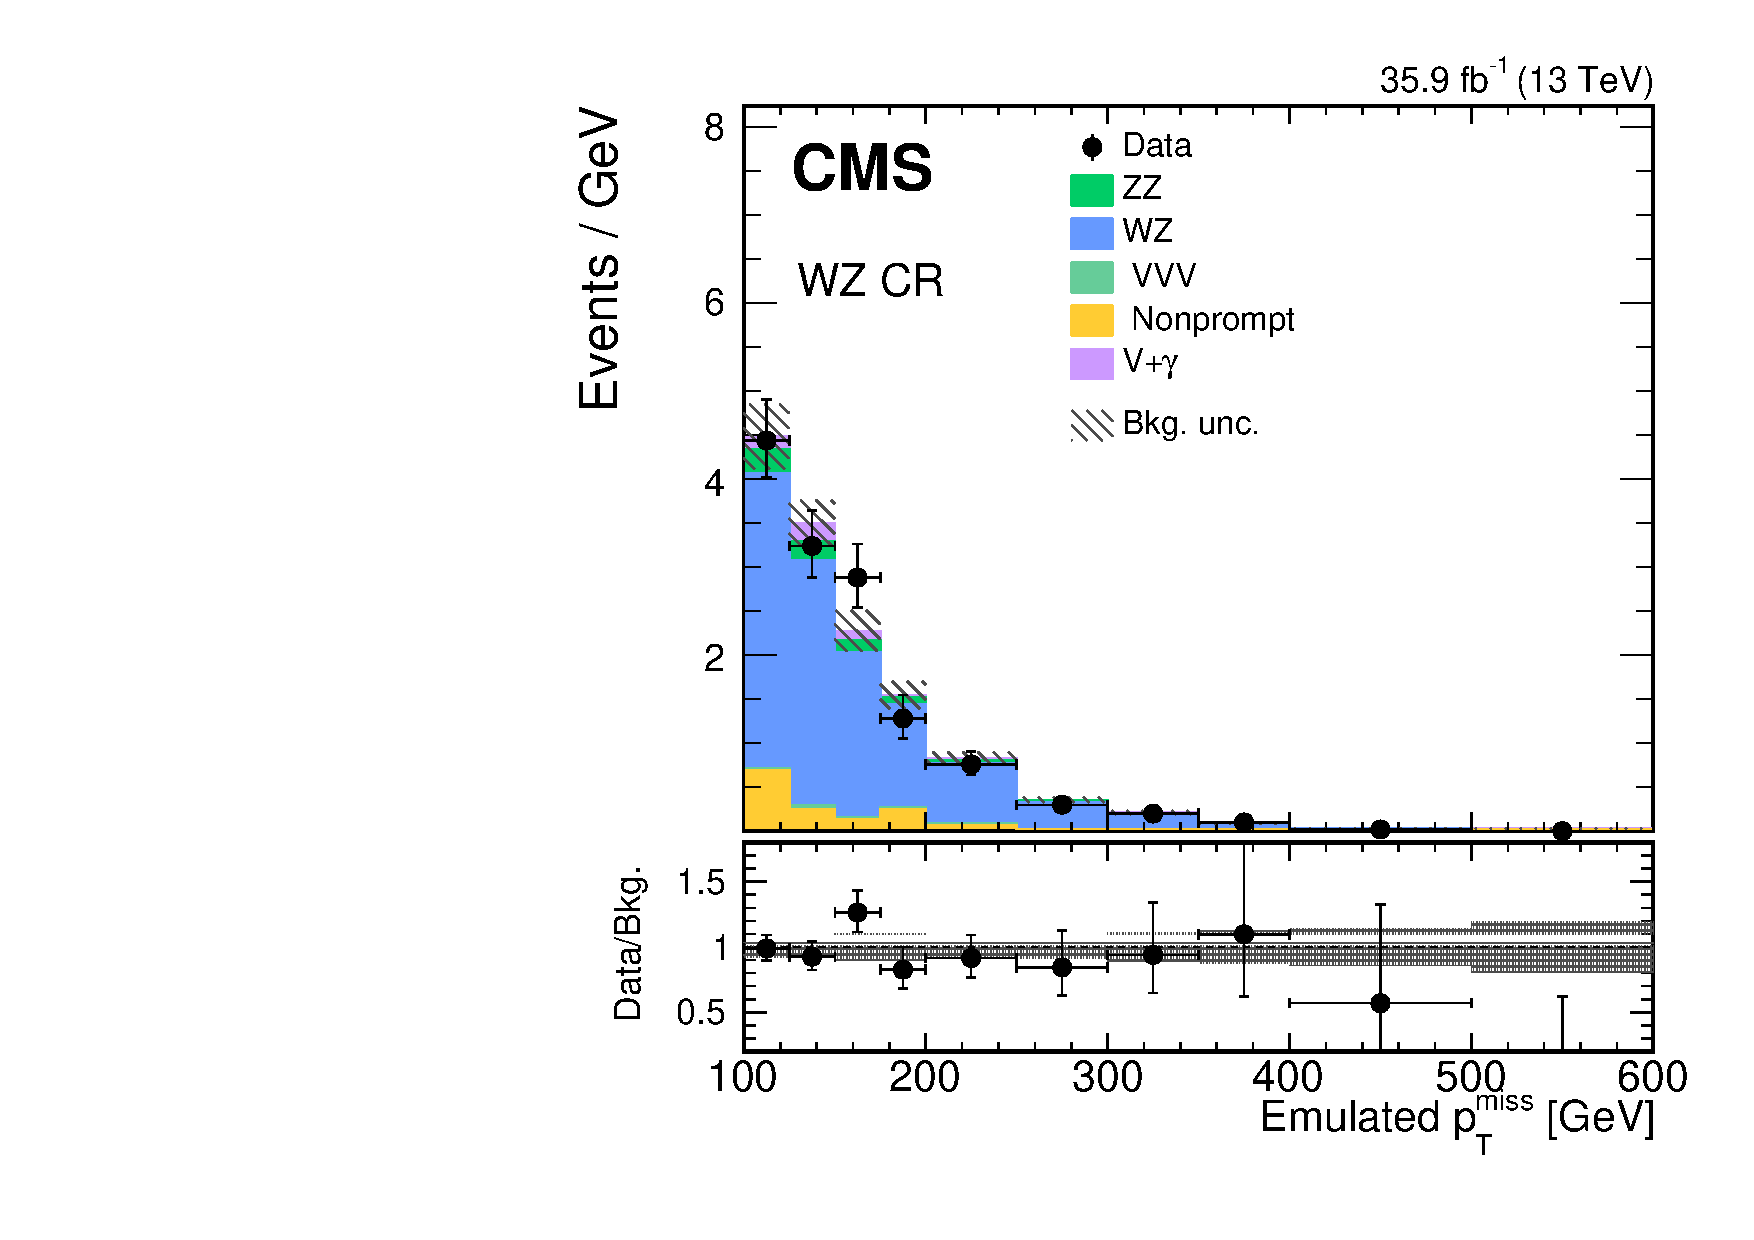
\includegraphics[width=0.48\textwidth]{figures/wz_fakemet_allcuts_postfit.pdf}
%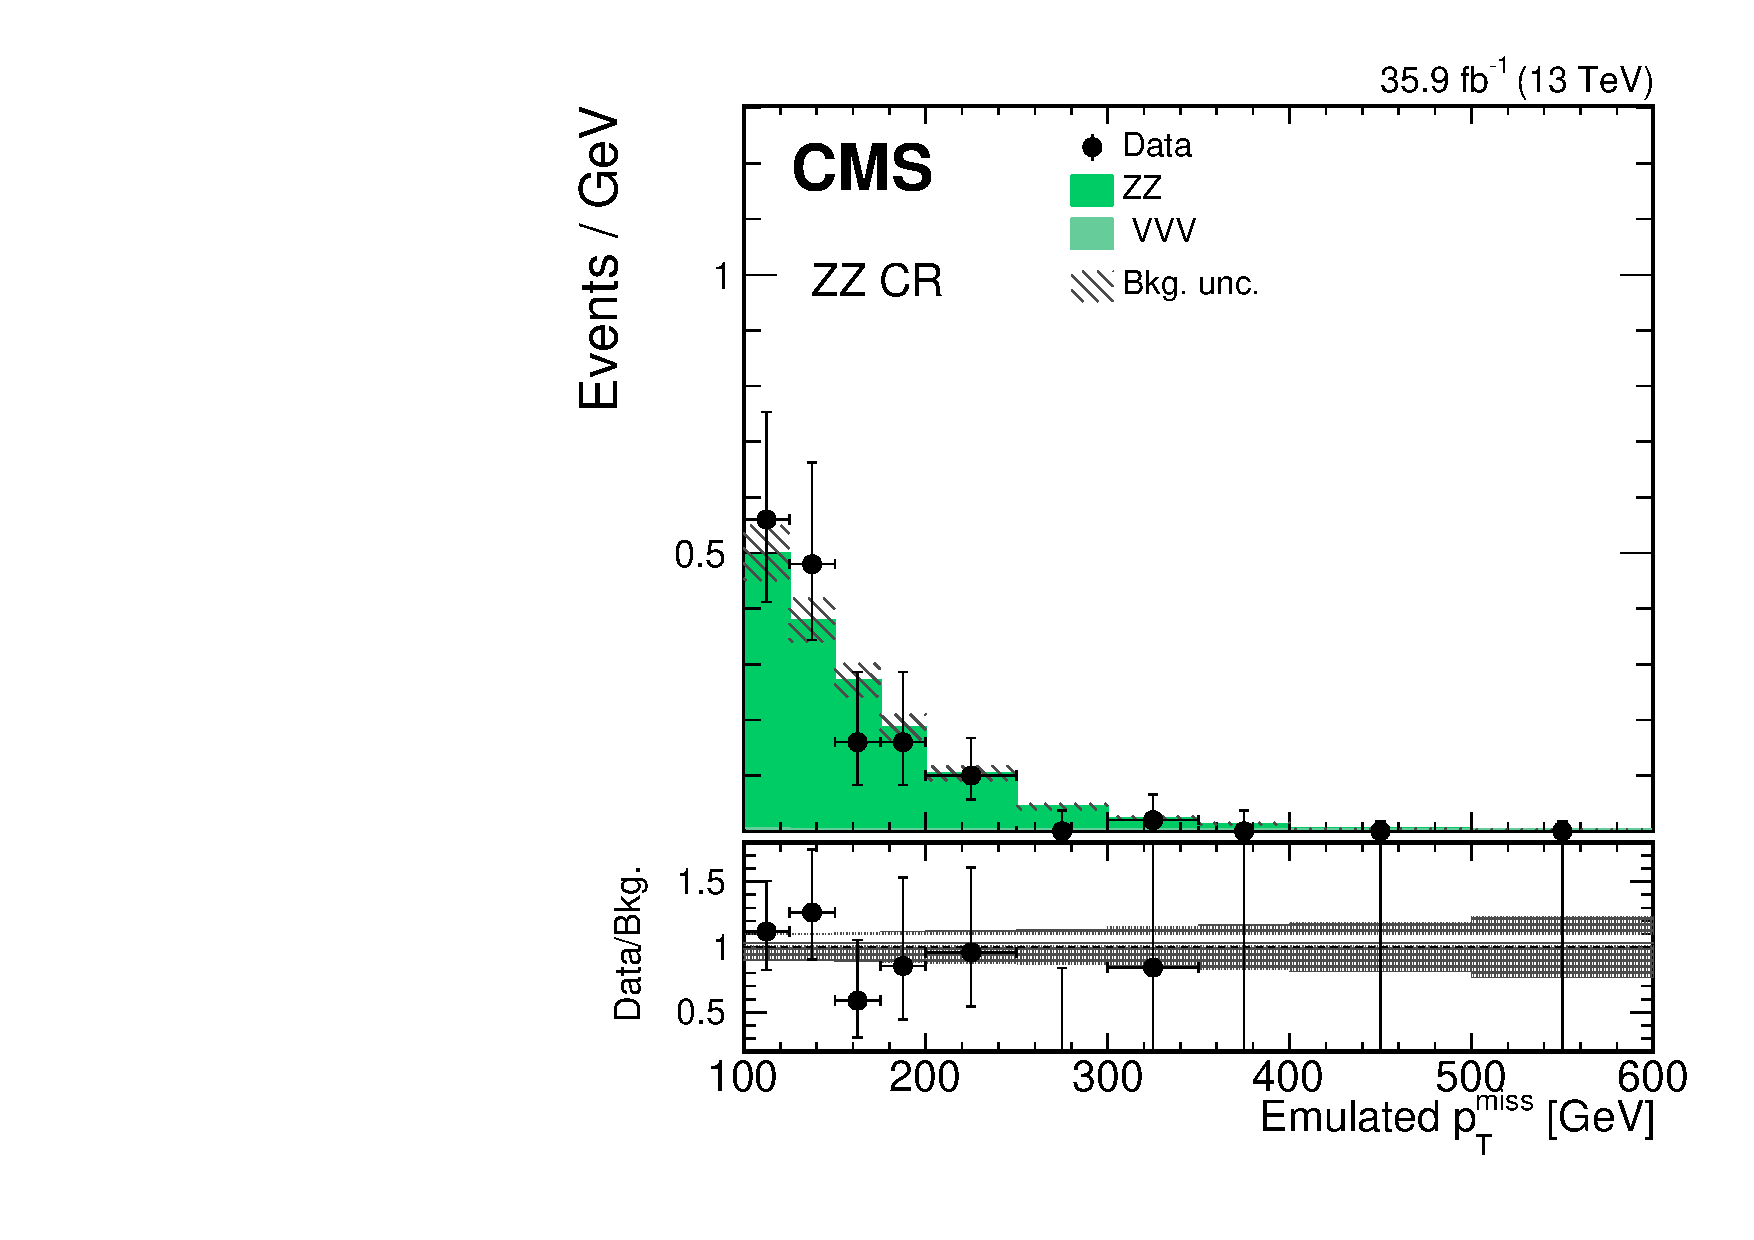
\includegraphics[width=0.48\textwidth]{figures/zz_fakemet_allcuts_postfit.pdf}
%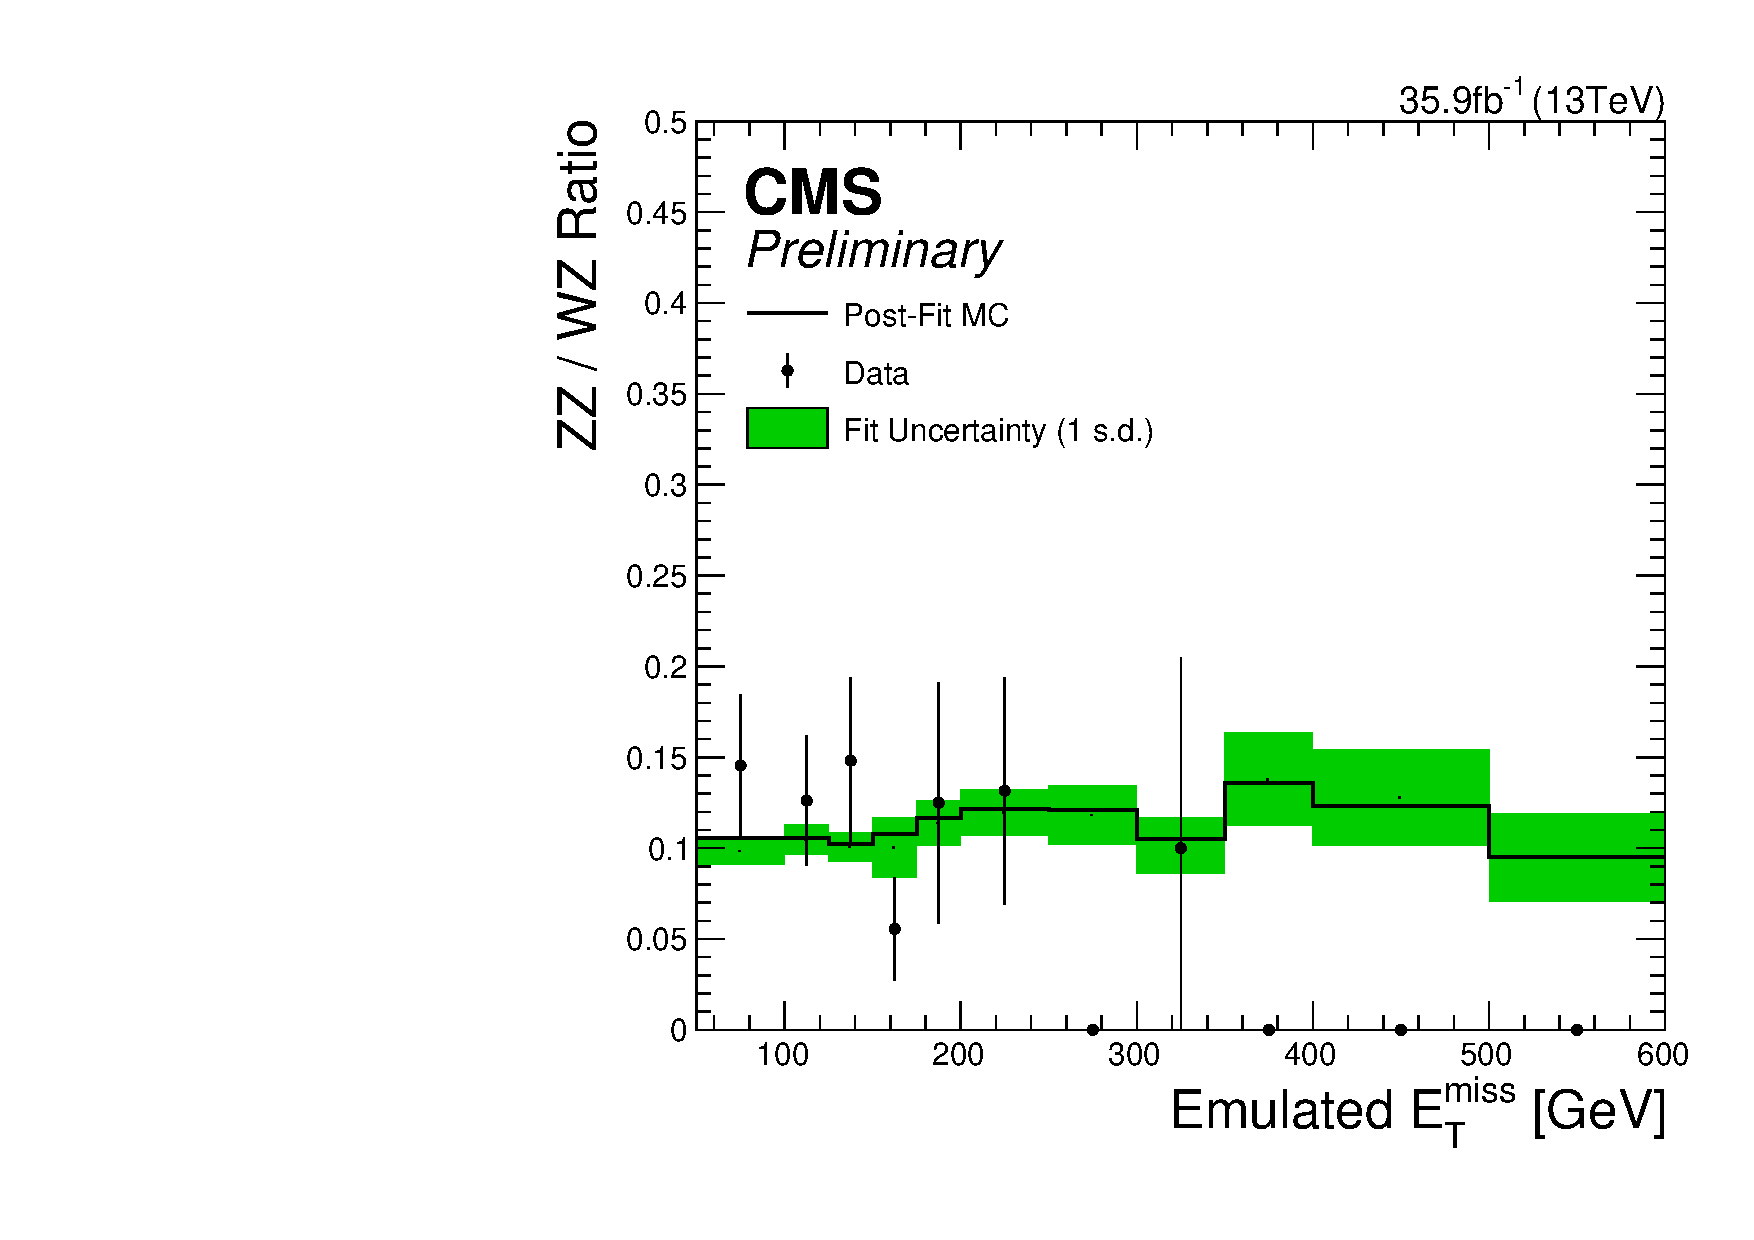
\includegraphics[width=0.48\textwidth]{figures/ratio_zzvswz.pdf}
%\caption{Emulated $\met$ 
%distribution for  the $\W\Z \to 3\Lep\nu$(top left) and $\Z\Z \to 4\Lep$ (top right) 
%control regions, and the ratio between both distributions in data and simulation (bottom).
% Uncertainty bands correspond to both statistical and systematic uncertainty.} 
%\label{fig:histo_fakemet}
%\end{figure}

\subsection{Nonresonant backgrounds}
The contribution of the non-resonant flavor symmetric backgrounds is  estimated from a control
sample of events with dilepton of different flavor
($\Pe^{\pm}\Pgm^{\mp}$) that pass all analysis selections.
Nonresonant backgrounds (NRB) consists mainly of leptonic \PW\ decays in
$\ttbar$, $\cPqt\PW$ decays and 
$\PW\PW$ events. Small contributions from single top-quark events produced from
$s$-channel and $t$-channel processes, and $\cPZ\rightarrow \Pgt\Pgt$
events in which $\Pgt$ leptons produce light leptons and \ETm are also
considered in this NRB estimation. 

The method assumes the lepton flavor symmetry in the final states of these processes.
Since the leptonic decay branching ratios for the $ee$, $\mu\mu$ and $e\mu$ final states from NRB are 1:1:2,
the $e\mu$ events selected inside the $\Z$-mass window can be extrapolated to the $ee$ and $\mu\mu$ channels.
To account for differences in efficiency for electrons and muons, a correction factor $k_{ee}$ can be derived
by comparing the NRB yields in the $ee$ and $\mu\mu$ channels:

\begin{equation}
k_{ee} = \frac{\epsilon_e}{\epsilon_{\mu}} \approx \sqrt{\frac{N^{ee}_{NRB}}{N^{\mu\mu}_{NRB}}}
\end{equation}
under the assumption is that each lepton leg acts independently.
In simulation, $k_{ee}$ is found to be about $0.88$ at final selection.
With this correction factor, the relation between the NRB yields in the signal and control region is:

\begin{equation}
\begin{split}
  N^{ee}_{NRB}     &= \frac{1}{2} k_{ee} N^{e\mu}_{NRB} \\
  N^{\mu\mu}_{NRB} &= \frac{1}{2} \frac{1}{k_{ee}} N^{e\mu}_{NRB} \\
\rightarrow N^{2\ell}_{NRB}  &= \frac{1}{2} \left( k_{ee} + \frac{1}{k_{ee}} \right) N^{e\mu}_{NRB} \\
&= f_{NRB} N^{e\mu}_{NRB}
\end{split}
\end{equation}
This transfer factor $f_{NRB}$ is implied by the MC estimates in the likelihood (Sec.~\ref{sec:likelihood}),
and the MC yields are found to be consistent (within the statistical uncertainty) with the derived relation.
Perturbations in the predicted transfer factor are suppressed upon summing the $ee+\mu\mu$ channels, as shown:
\begin{equation}
\begin{split}
  f + \delta f &= \frac{1}{2} \left( k + \delta k + \frac{1}{k + \delta k} \right) \\
  &= f + \frac{k^2-1}{2k^2} \delta k + \mathcal{O}(\delta^2) \\
  &= f + \mathcal{O}(\delta^2) \quad \text{for } k \approx 1
\end{split}
\end{equation}
such that the extrapolation uncertainty, taken as a conservative 20\%, easily covers any data-MC discrepancy
in the transfer factor.

Note that the $e\mu$ control sample contains a small contribution from
$\PW+{\mathrm{jets}}$ because of fake leptons. Since the rate of fake
electrons and muons is different, this method does not account
properly for the $\PW+{\mathrm{jets}}$ contribution, leading to an
underestimation of $\PW+{\mathrm{jets}}\to ee+X$, and an
overestimation of $\PW+{\mathrm{jets}}\to \mu\mu+X$. Given the very 
small yield expected for such process in the signal region, well below
the systematic uncertainty, the effect can be safely
neglected. Moreover, the small biases resulting in the $ee$ and
$\mu\mu$ channels partially cancel out, so the overall effect on the
$\Lep\Lep$ channel is even smaller. 

As shown in Fig.~\ref{fig:m_em},
the $e\mu$ invariant mass, transverse momentum distributions and the \met\ distribution in
the $e\mu$ channel, the dominant sources in the $e\mu$ channel within
the Z mass window and in large $\ETm$ (or $p_{T}^{\Lep\Lep}$) region are
$t\bar t, \ tW, \ WW $, $\tau\tau$, and $\PW+{\mathrm{jets}}$ events. Contributions from the $t\bar t Z$ process
are deemed negligible.
As shown in Fig.~\ref{fig:met_tt_ww}, the shape of the $\met$ spectrum is identical in the $e\mu$ control region
and the $\ell\ell$ signal region.


\begin{figure}[!h]
 \begin{center}
   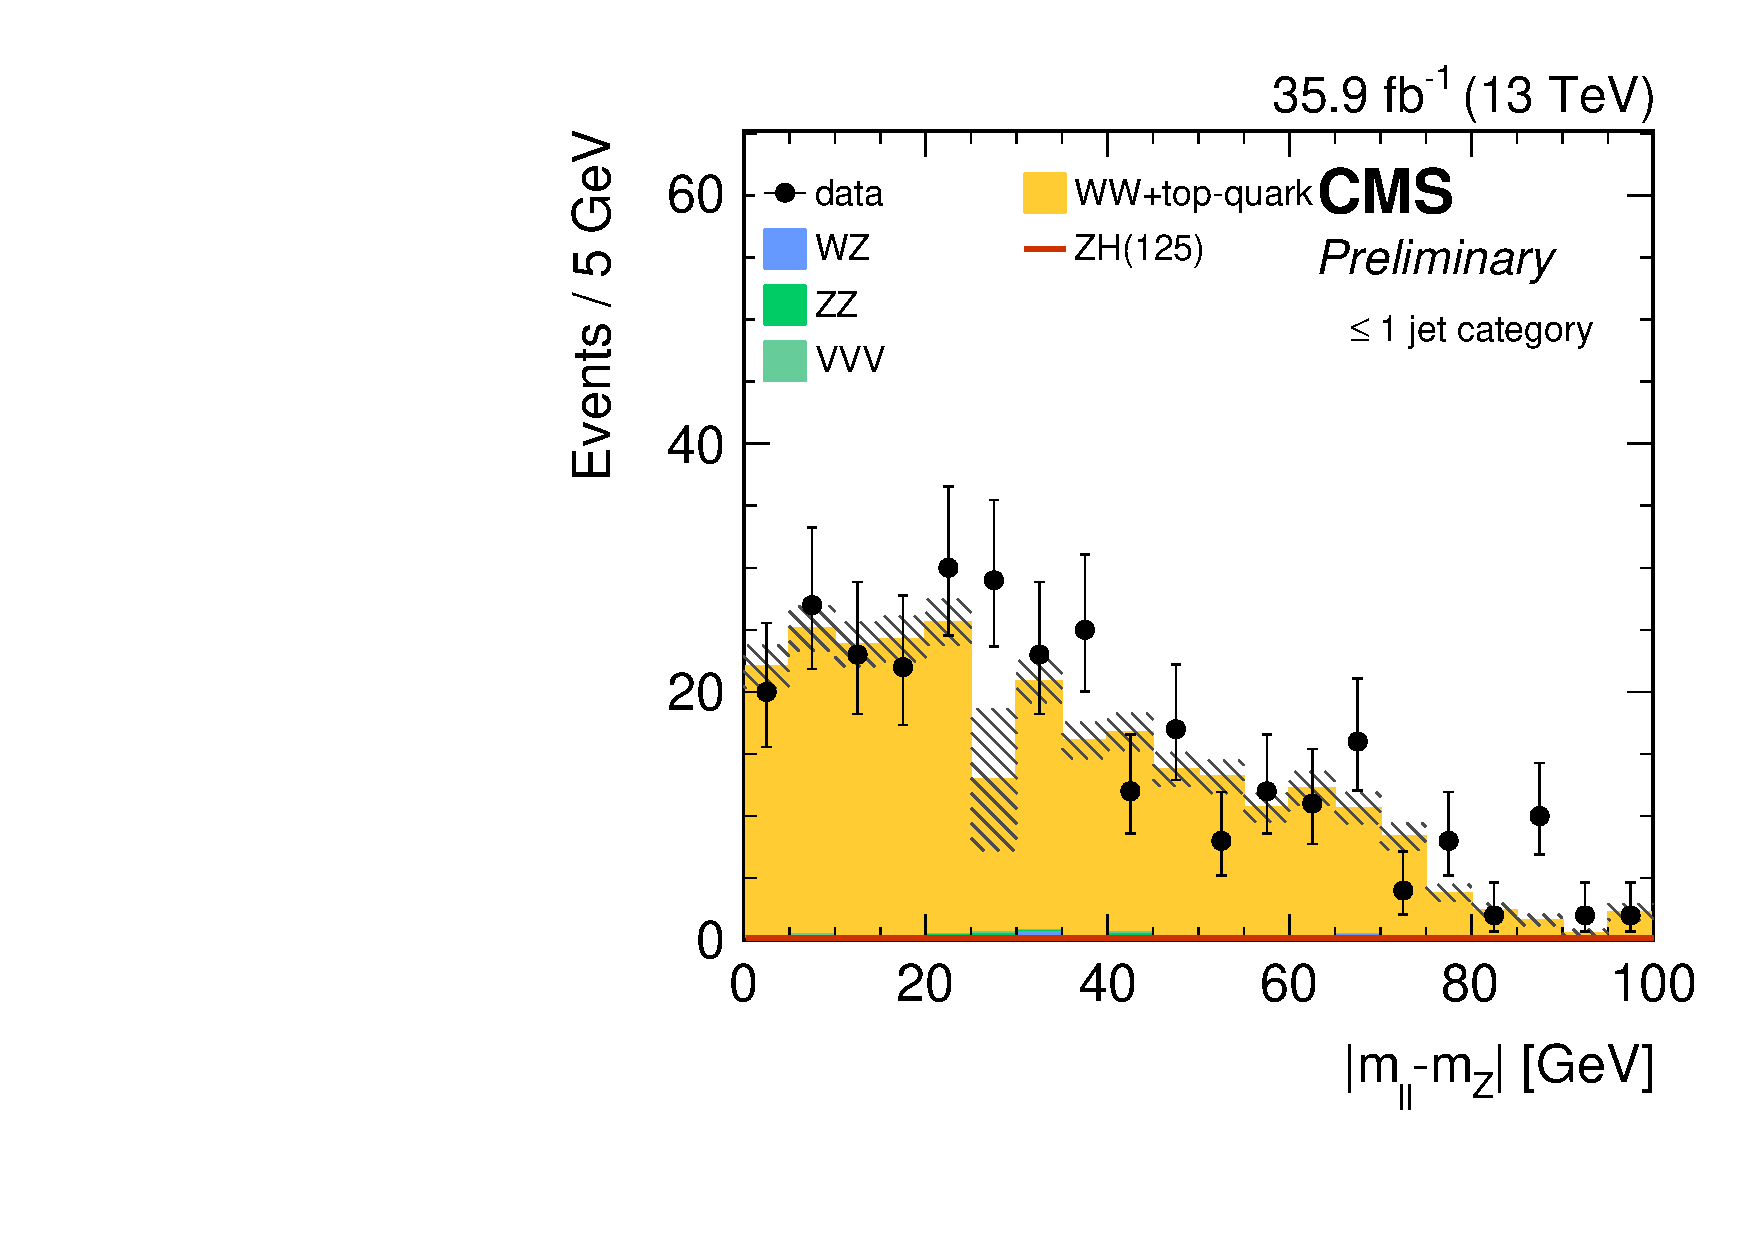
\includegraphics[width=0.46\textwidth]{figures/em_zh_1j_mll_allcutsbutone.pdf}
   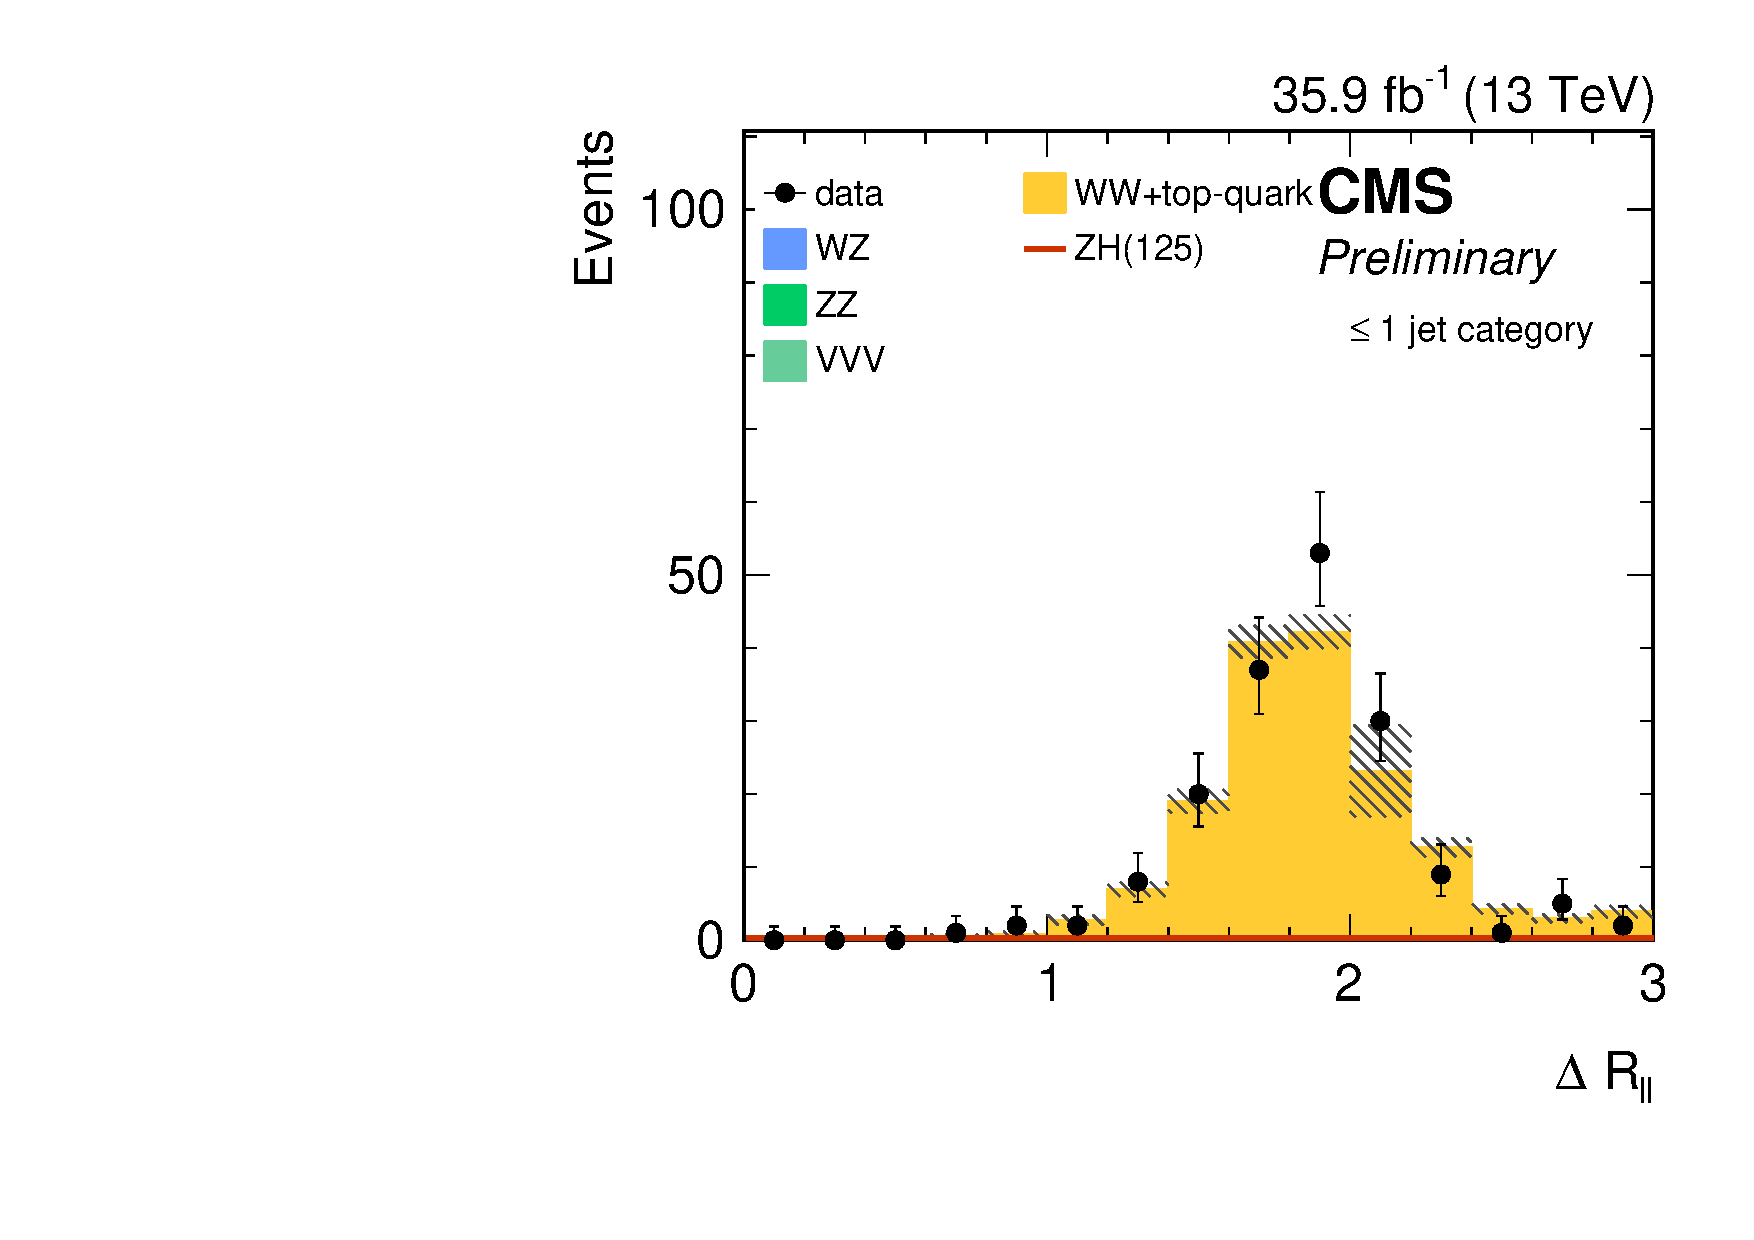
\includegraphics[width=0.46\textwidth]{figures/em_zh_1j_deltarll_allcutsbutone.pdf}\\
   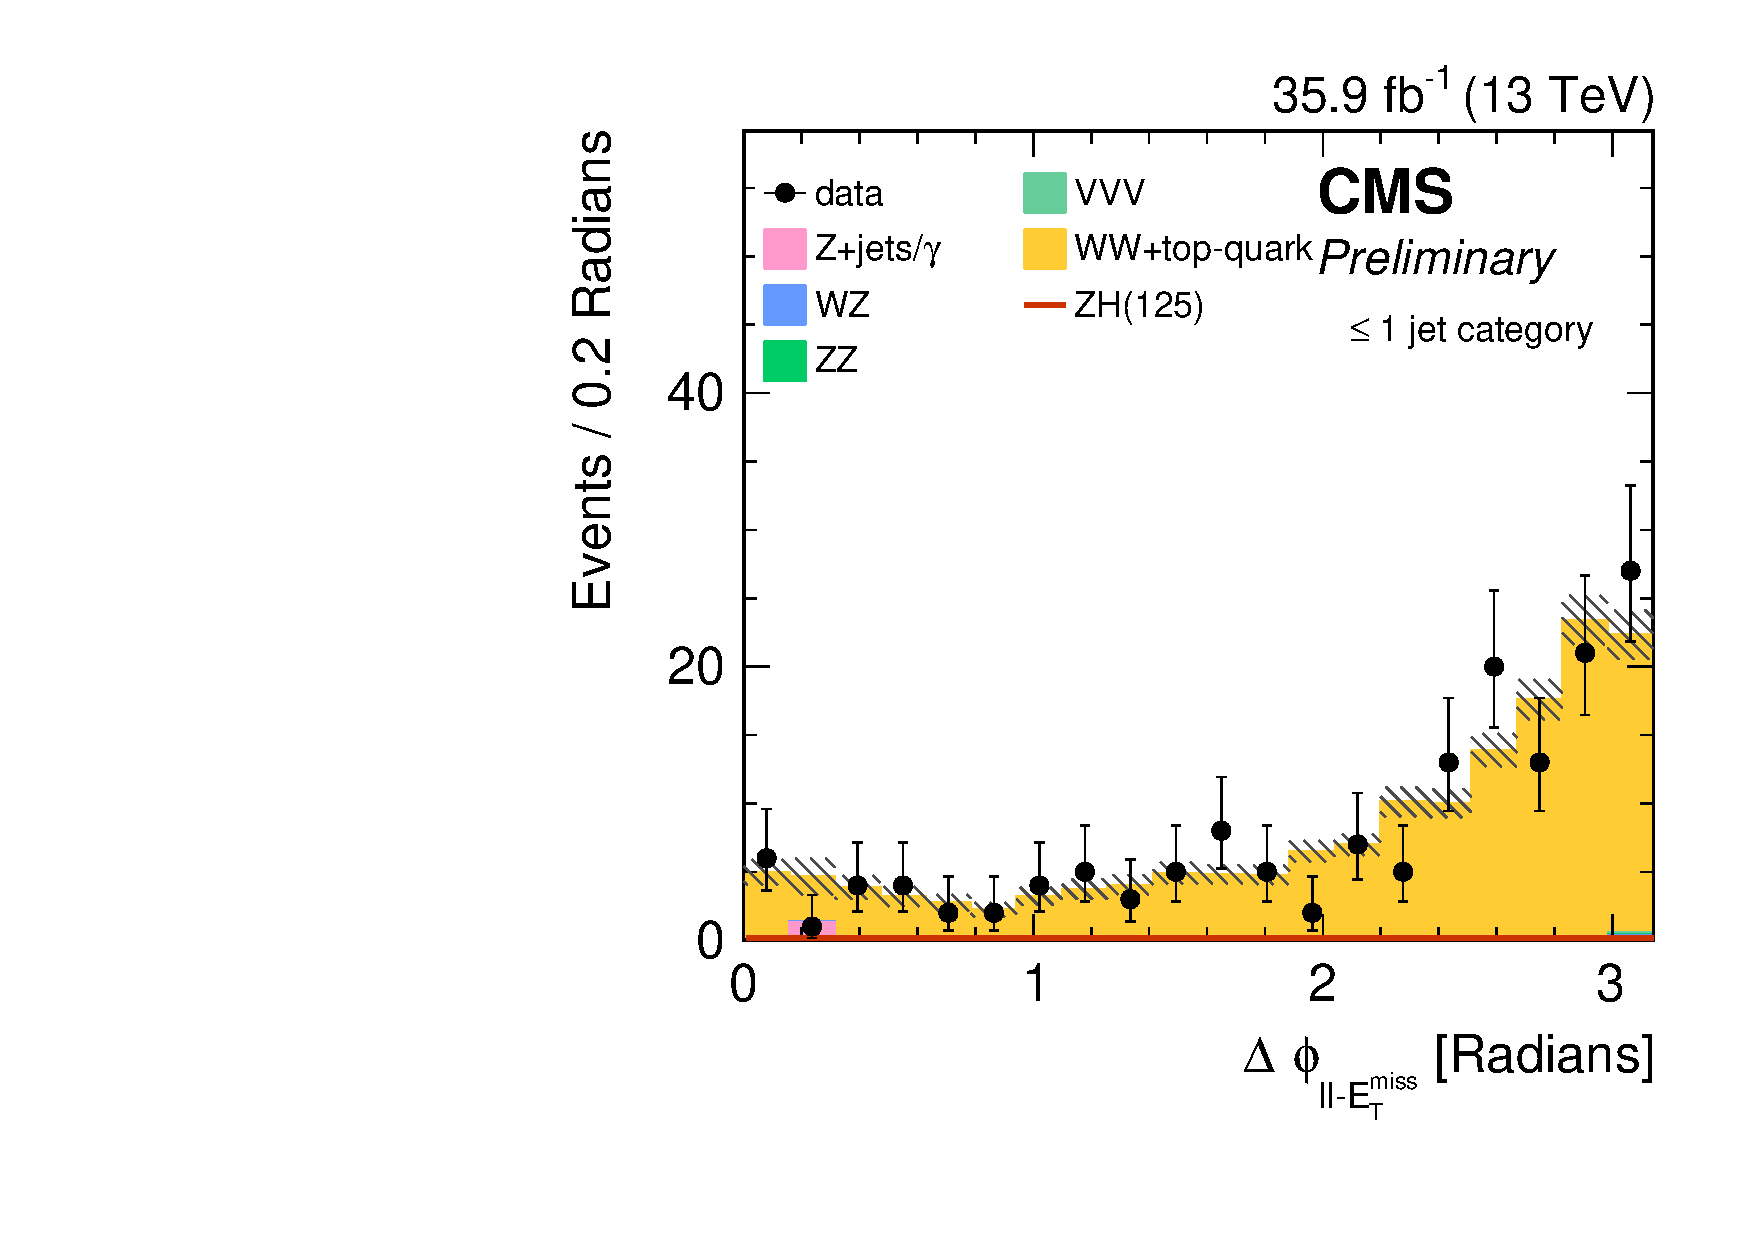
\includegraphics[width=0.46\textwidth]{figures/em_zh_1j_dphillmet_allcutsbutone.pdf}
   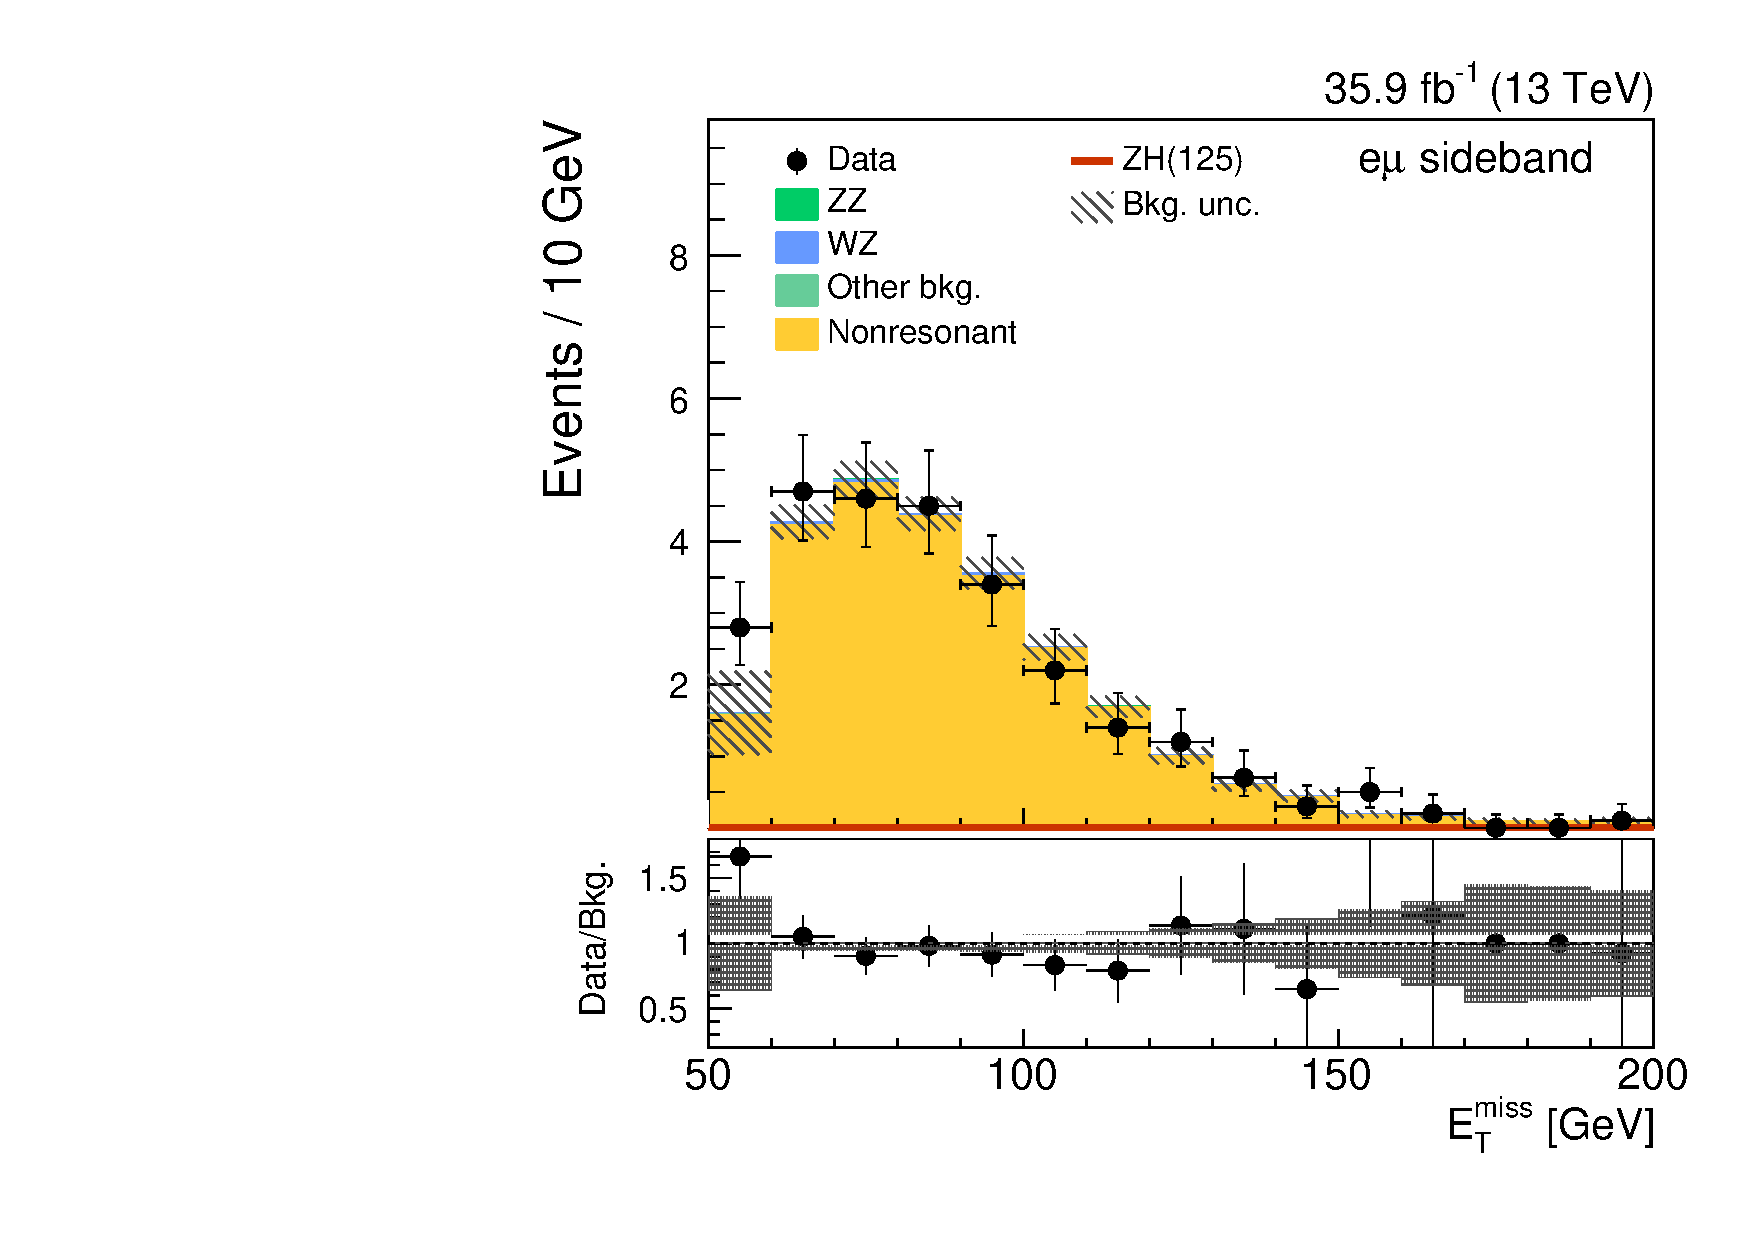
\includegraphics[width=0.46\textwidth]{figures/em_zh_1j_met_allcutsbutone.pdf}
 \end{center}
 \caption{Distributions of $|m_{e\mu}-m_{\Z}|$,
        $\Delta R_{\ell\ell}$,
        $\Delta \phi_{\ell\ell,\met}$,
        and $\met$ for $\Pe \mu$ events after applying the full selection except the variable itself.}
\label{fig:m_em}
\end{figure}

\begin{figure}[hb]
\centering
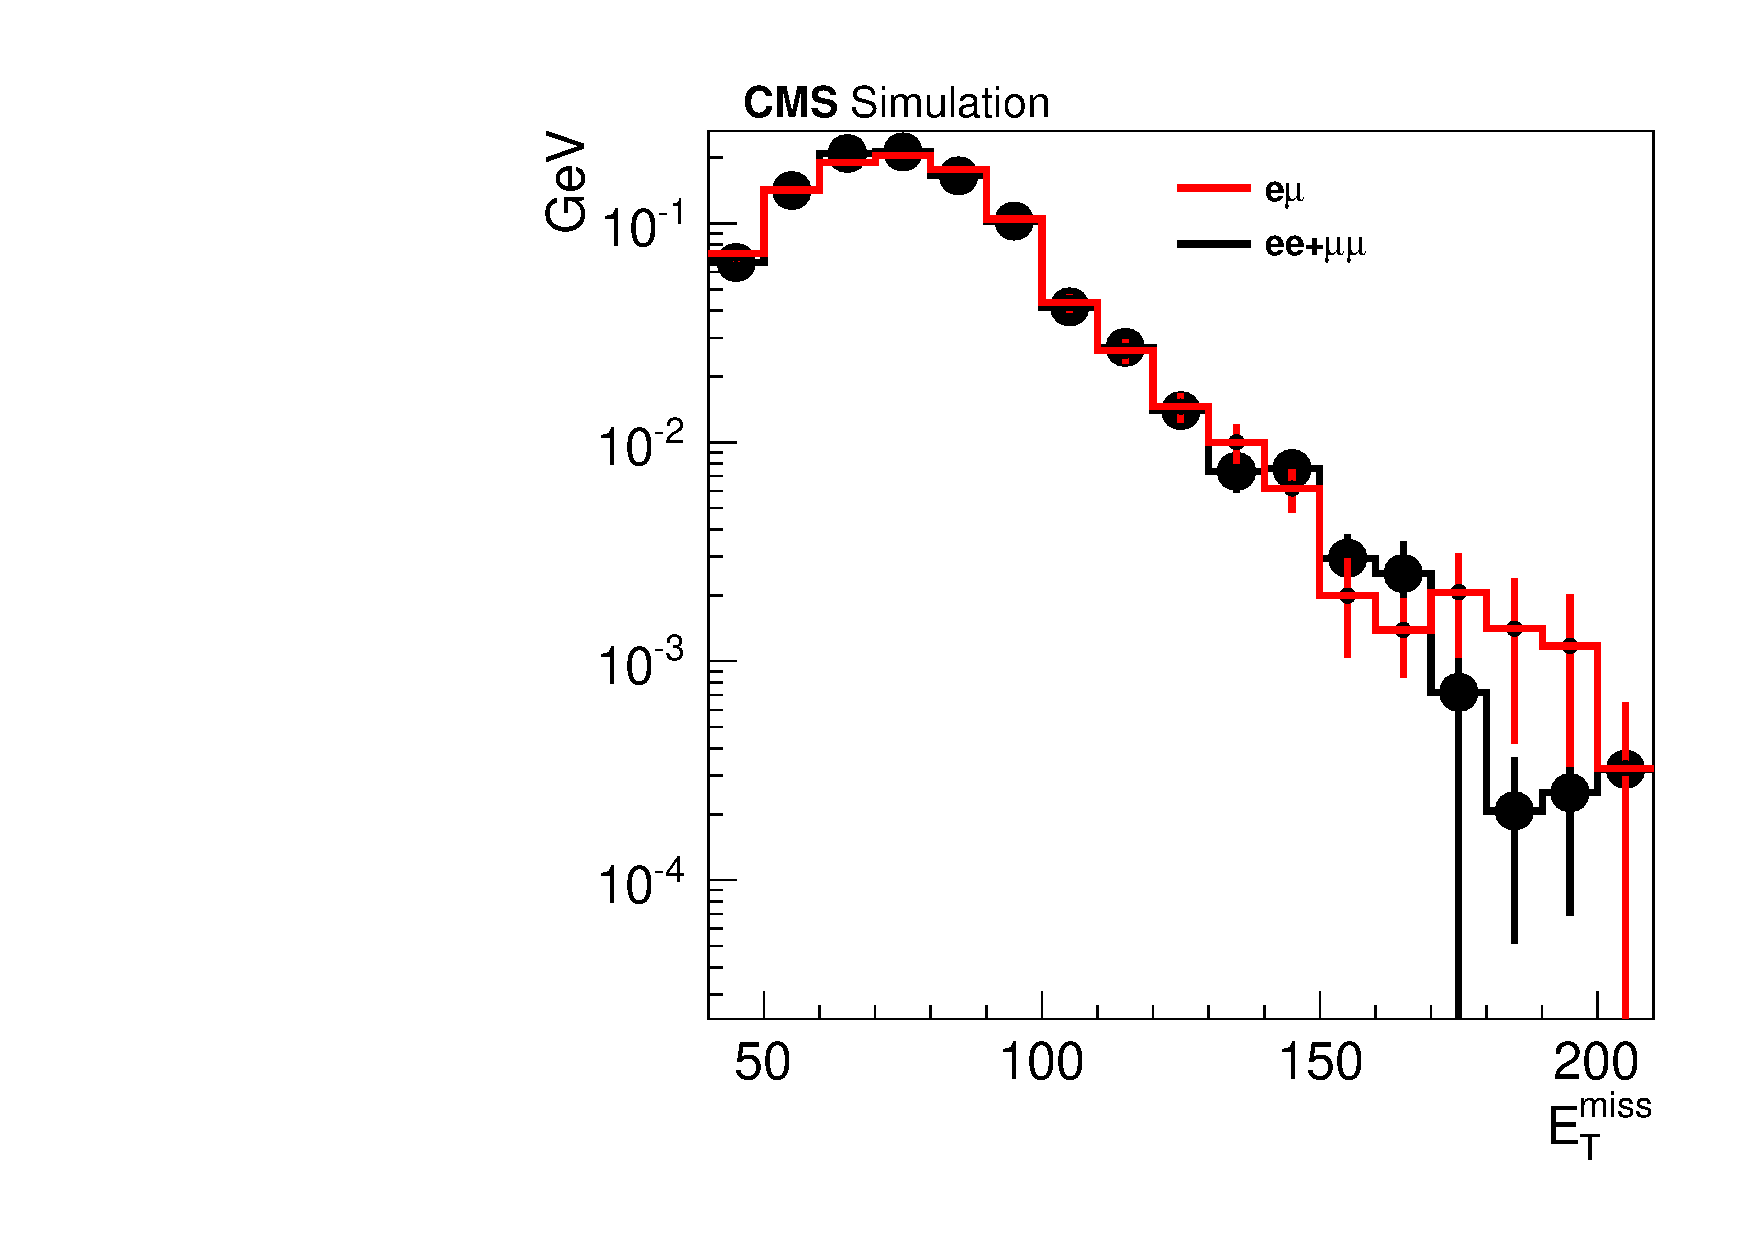
\includegraphics[width=0.48\textwidth]{figures/met_tt_ww.pdf}
\caption{Comparison of the $\met$ distributions for $\WW$+top-quark simulated 
events for $e\mu$ versus $ee+\mu\mu$ events.} 
\label{fig:met_tt_ww}
\end{figure}

\newpage
\subsection{Drell-Yan background estimation}
The Drell-Yan (DY) process is dominant in the region of low $\ETm$.
This process does not produce undetectable particles, therefore any non-zero $\ETm$ arises from
limited detector acceptance and mismeasurement.
The estimation of this background uses simulated DY events, which are normalized to data in a control region.
A scale factor is obtained by measuring the number of DY events in a $\met$ sideband of $[50, 100]\GeV$,
and is included in the maximum likelihood fit, as shown in Sec.~\ref{sec:likelihood}.

A $100\%$ (i.e. factor of two) uncertainty is assigned to the DY estimate in order to cover the extrapolation from the low-\met region to the higher-\met signal region.
This uncertainty has little effect on the results due to the small overall contribution from the DY process.
Extensive checks have been performed to ensure that the estimation method is sensible.
By defining control regions where $\met$ mismodeling issues are expected to have a large impact, and confirming that the 
estimate from simulation for these regions still holds within the uncertainties, it is shown in Fig.~\ref{fig:met_control} that $\met$ mismodeling is under control.
Additionally, an independent estimation method using a $\gamma+\met$ control region was implemented, and the results were 
confirmed to be consistent between the two methods, further increasing confidence in the approach chosen here.
%Detailed information regarding the $\gamma+\met$ studies can be found in~\cite{CMS-AN-2016-199}.

Spurious muons and mismeasured electrons were observed in the re-reconstruction of the 2016 data, due to the relaxed tracking and PF requirements of the `HIP mitigation.'
A `re-MINIAOD' re-analysis of the data was performed to identify and clean or correct the data for these objects.
These issues are not expected to affect our analysis in a significant manner, mainly due to our third lepton veto.
Nevertheless, we checked that the effect is negligible in our signal region, and a correlation plot showing the effect of this cleaning is shown in Fig.~\ref{fig:met_control}.

\begin{figure}[hb]
  \centering
  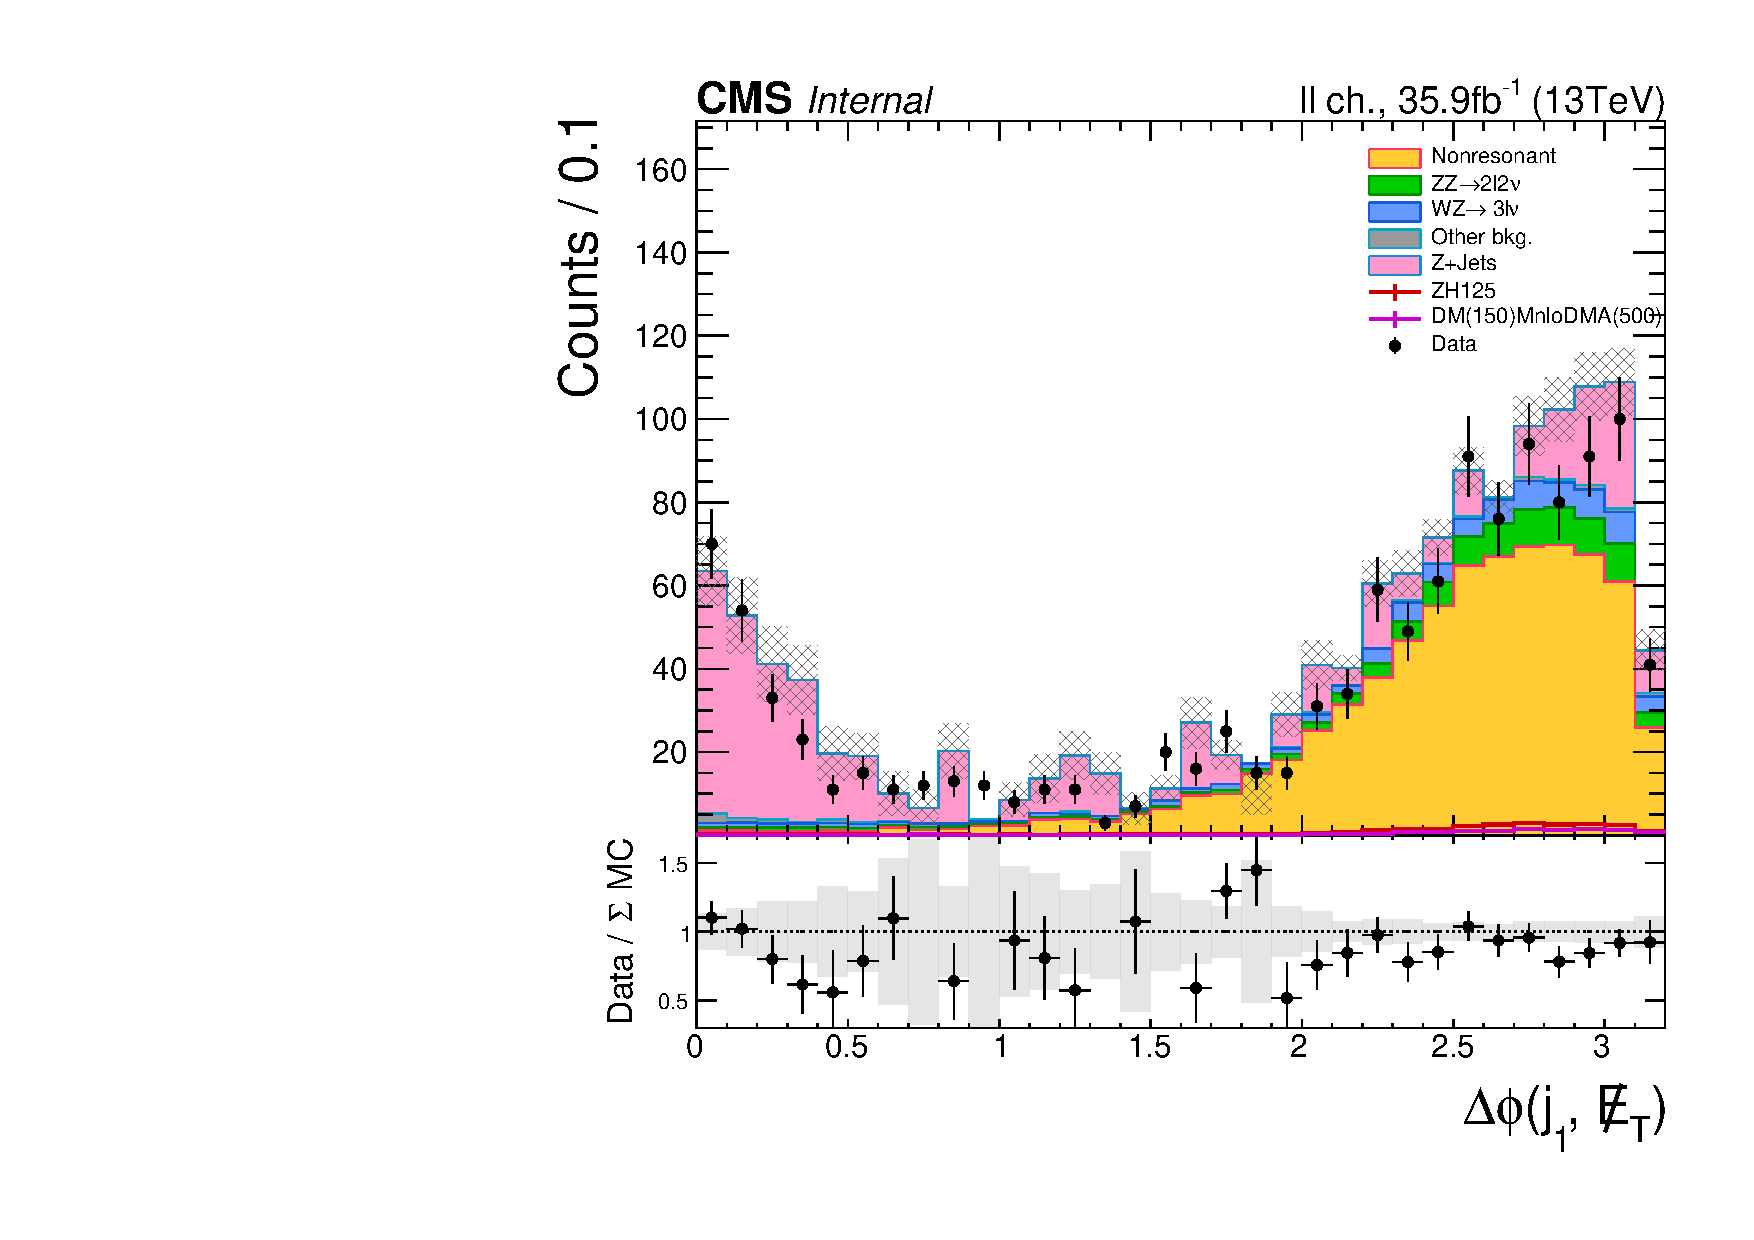
\includegraphics[width=0.48\textwidth]{figures/ll_metCheck_dPhiJetMet_failBalance.pdf}
  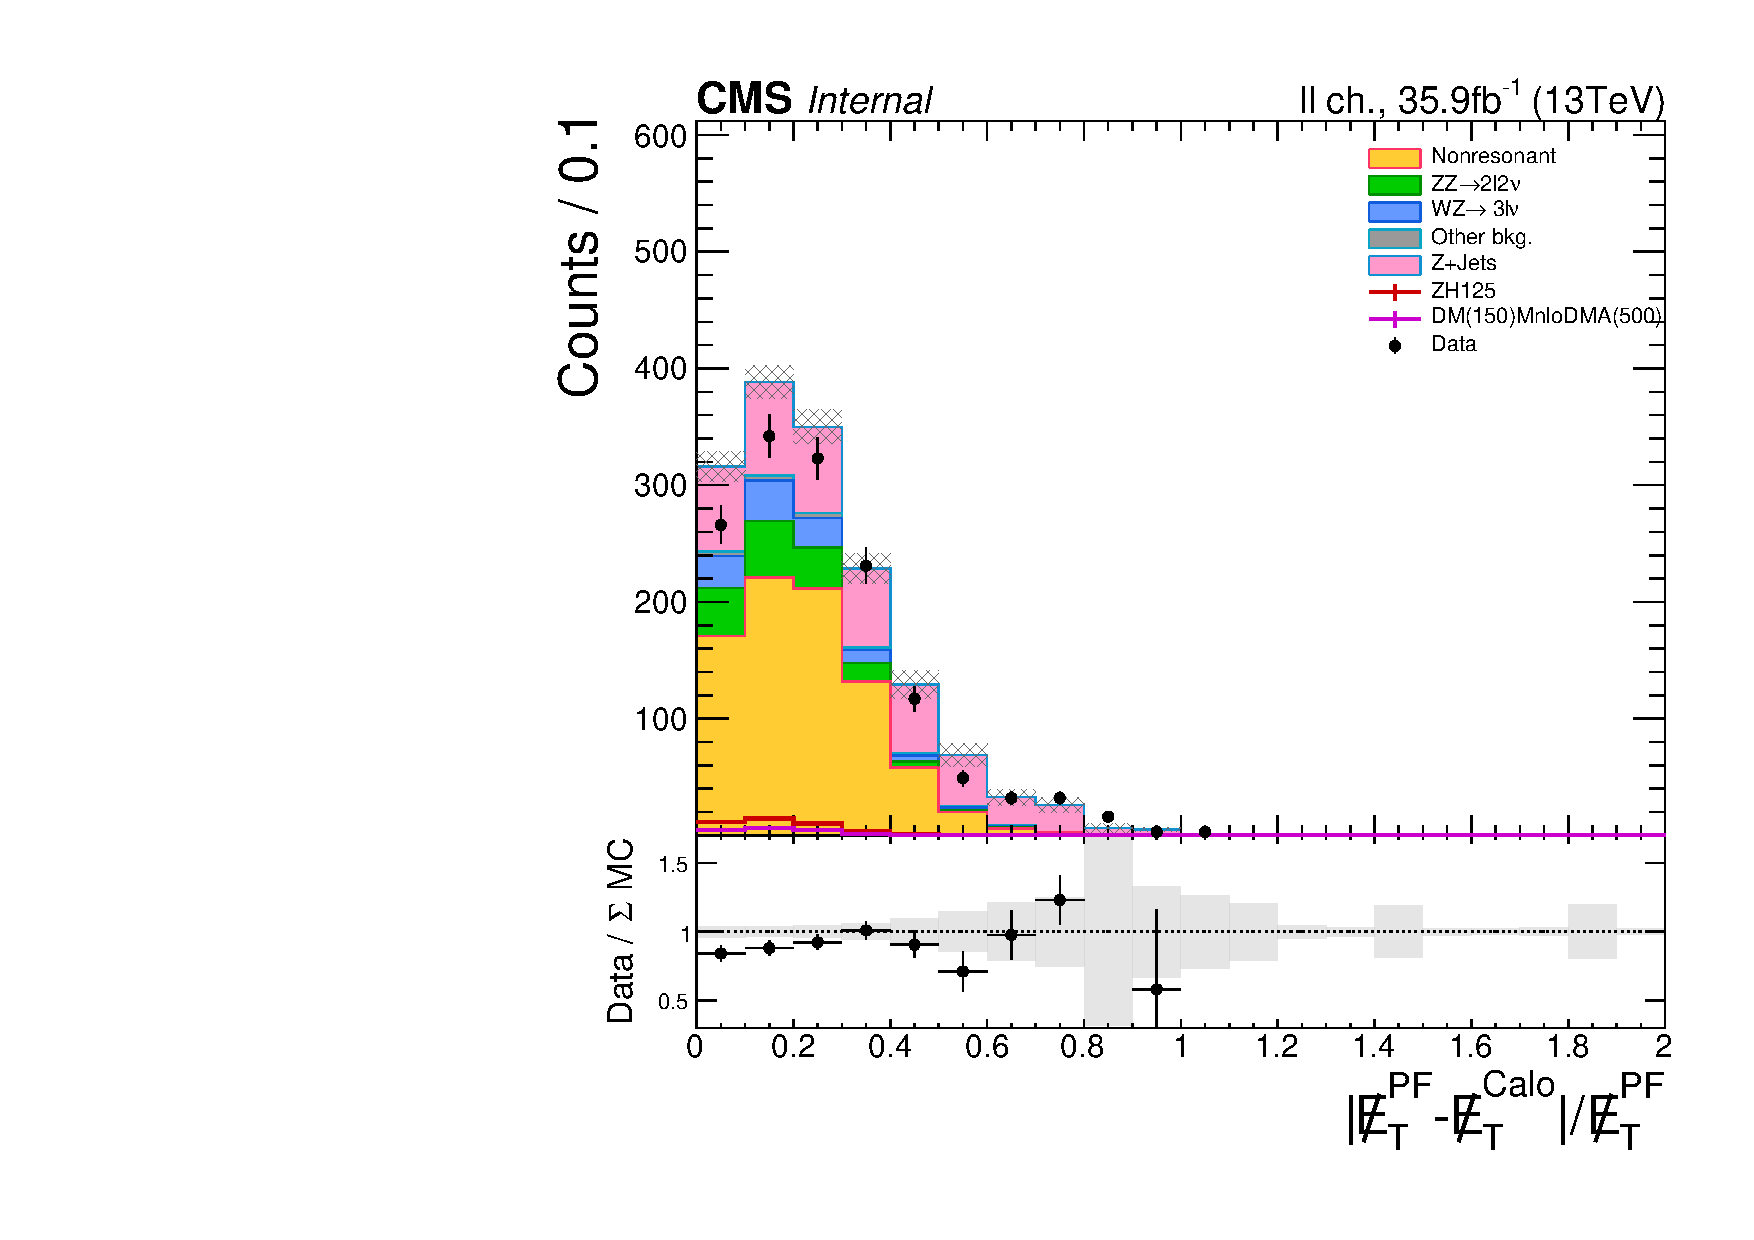
\includegraphics[width=0.48\textwidth]{figures/ll_metCheck_pfVsCaloMet_failBalance.pdf}
  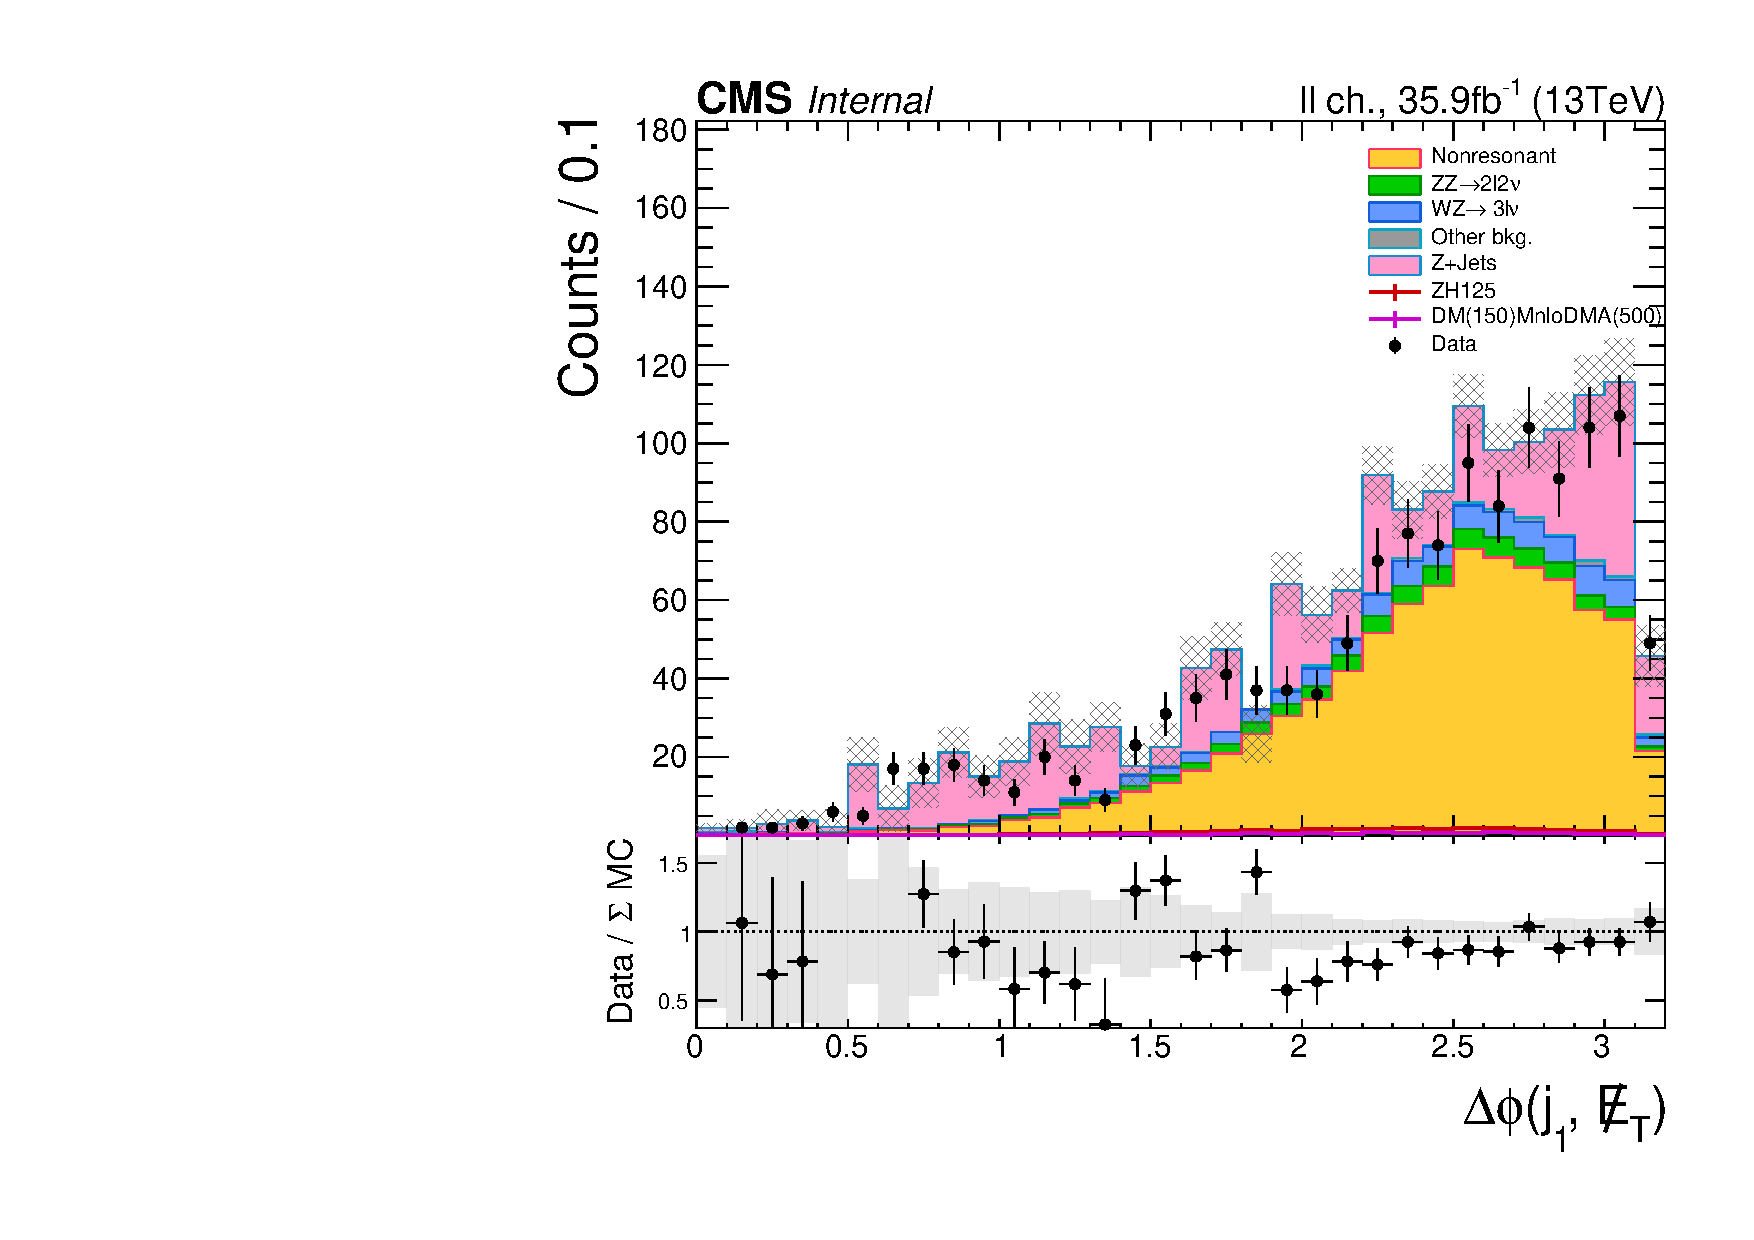
\includegraphics[width=0.48\textwidth]{figures/ll_metCheck_dPhiJetMet_failDphi.pdf}
  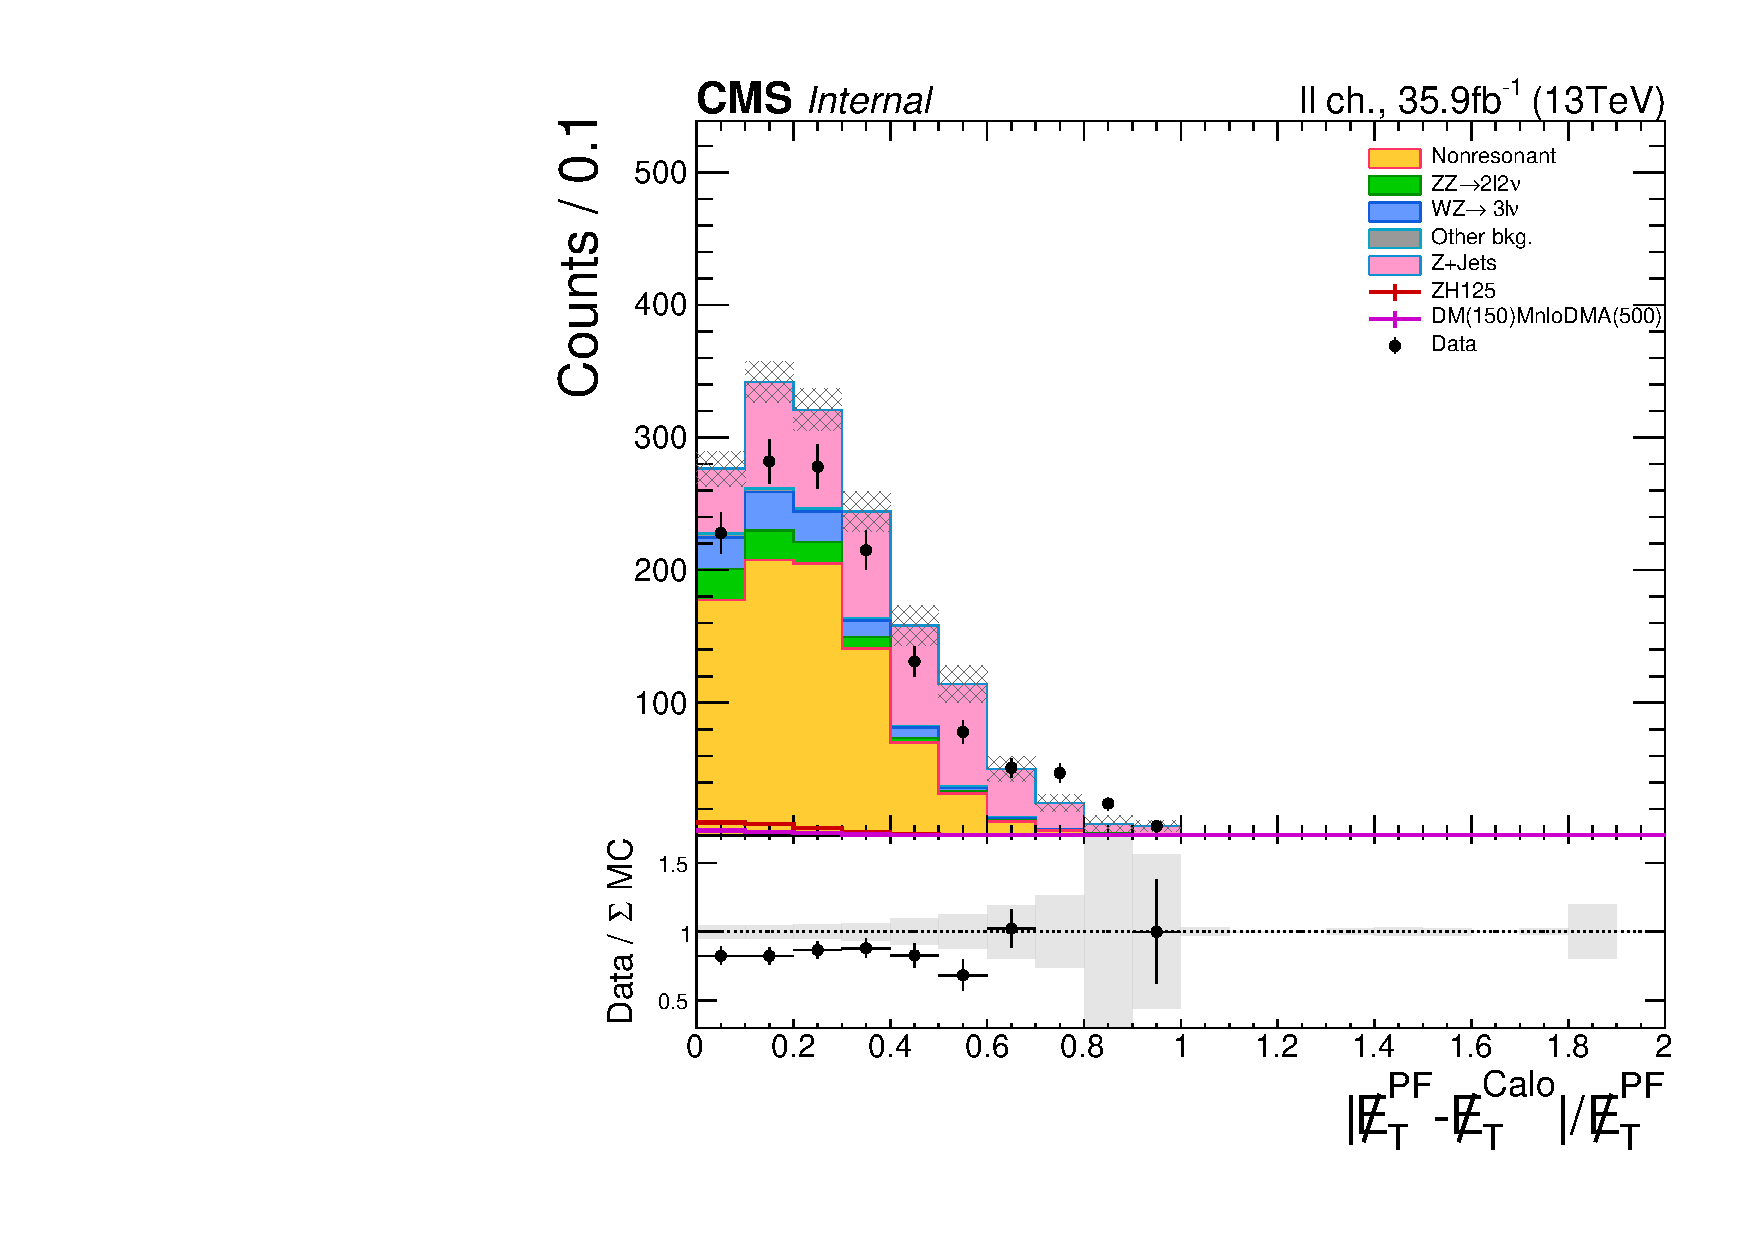
\includegraphics[width=0.48\textwidth]{figures/ll_metCheck_pfVsCaloMet_failDphi.pdf}
  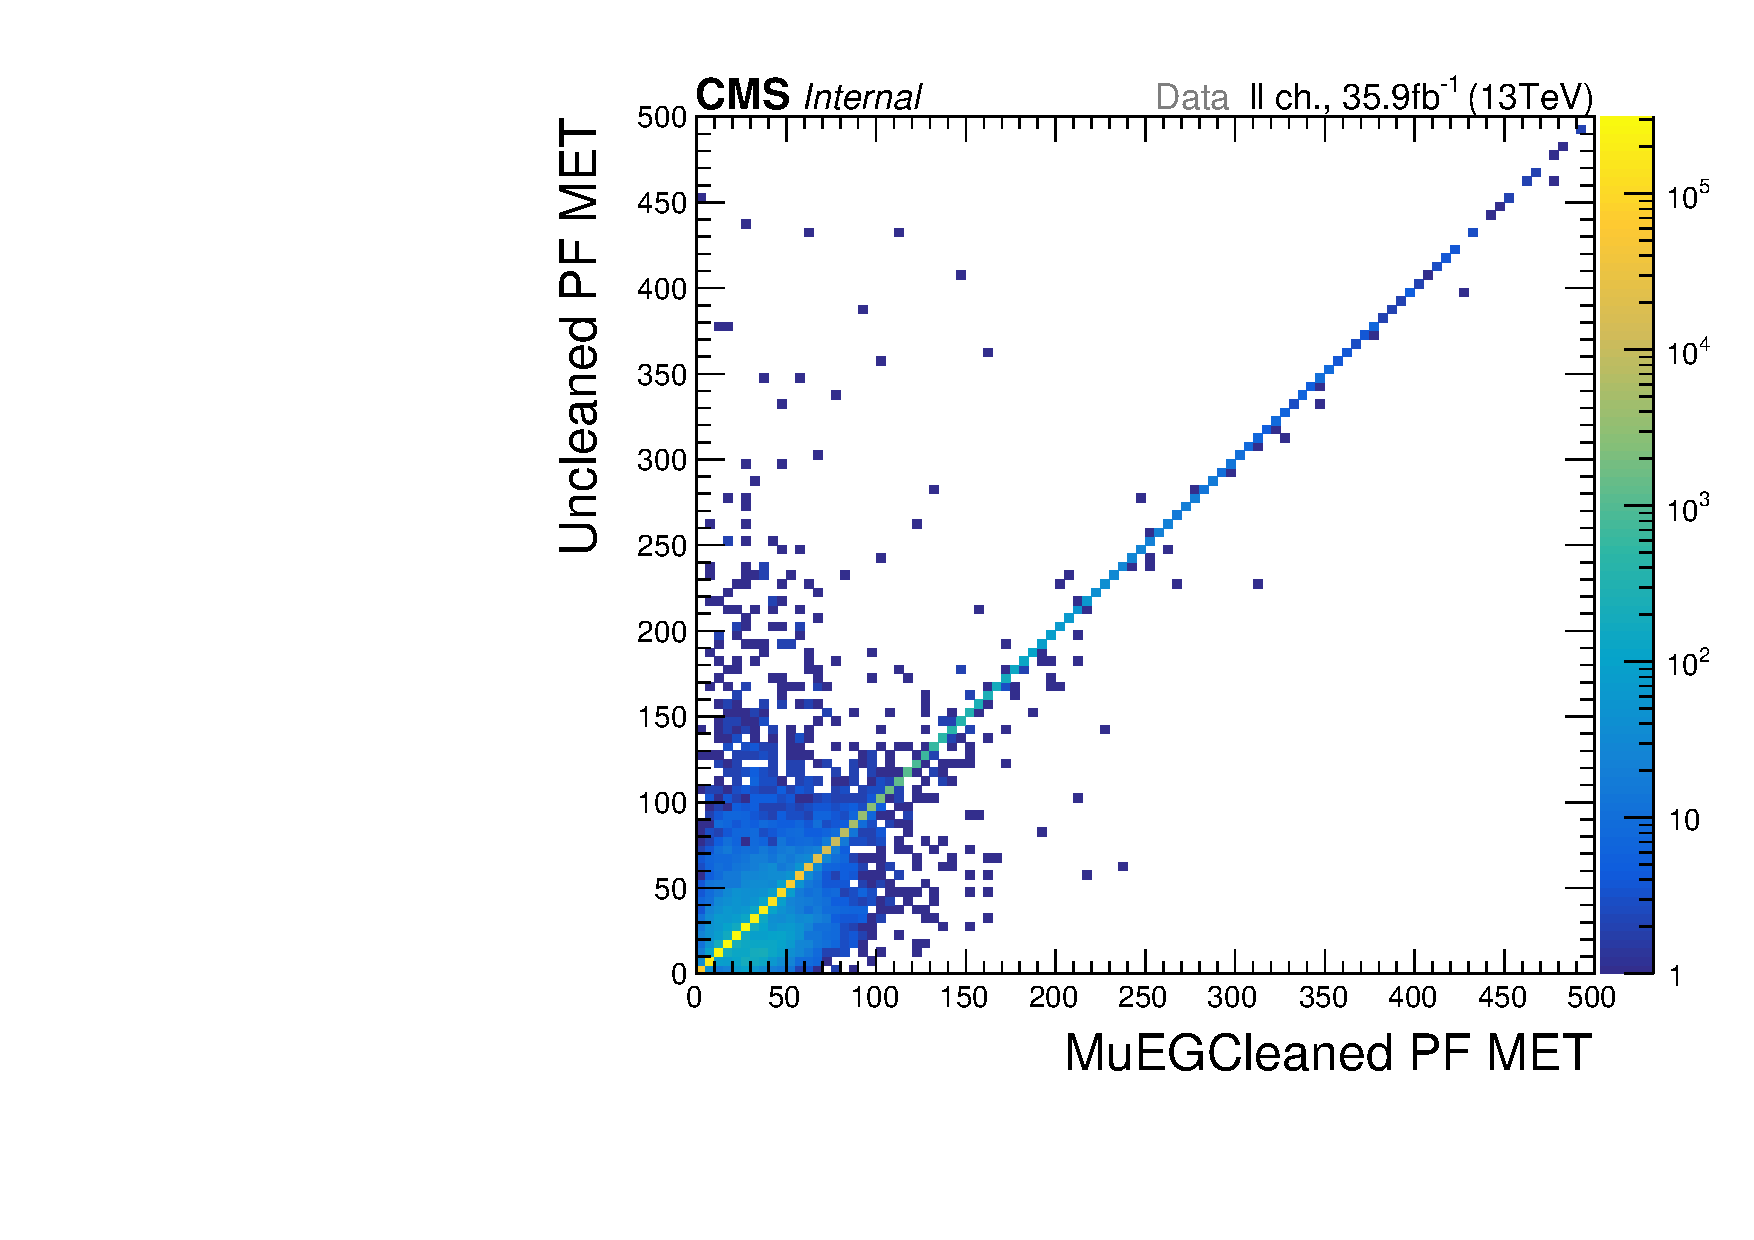
\includegraphics[width=0.48\textwidth]{figures/ll_metAltVsUncleaned.pdf}
  \caption{
    Selection of MET mismodeling control regions, after a loose selection: $m_Z$ window, $p_{T}^{\ell\ell}>60\GeV$, $<2$ Jets, $\met>100\GeV$.
    Top row: Events failing MET Balance cut, $\Delta\phi(j,\met)$ and the PF to Calo MET ratio are plotted.
    Second row: Events failing $\Delta\phi(Z,\met)$ cut, $\Delta\phi(j,\met)$ and the PF to Calo MET ratio are plotted.
    Last row: Correlation between \met and the cleaned \met from the re-MINIAOD campaign, showing the effect of the cleaning.
  }
  \label{fig:met_control}
\end{figure}



\section{Systematic uncertainties}
\section{Maximum likelihood fit}
\label{sec:likelihood}
The likelihood $\mathcal{L}$ is constructed as follows:
\begin{equation}
\begin{split}
  \mathcal{L} = \prod_{i} \mathcal{P}&\termLB N^{2\ell}_{obs,i} \bigg| \boldsymbol\mu_{DY} N^{2\ell}_{DY,i}(\boldsymbol\theta) + \boldsymbol\mu_{NRB} N^{2\ell}_{NRB,i}(\boldsymbol\theta) \\
  & + N^{2\ell}_{other,i}(\boldsymbol\theta) + \boldsymbol\mu_i^{VV} (N^{2\ell}_{ZZ,i}(\boldsymbol\theta)+N^{2\ell}_{WZ,i}(\boldsymbol\theta)) + \boldsymbol\mu N^{2\ell}_{Sig,i}(\boldsymbol\theta) \termRB \\
   \times \prod_{i} \mathcal{P} & \termLB N^{3\ell}_{obs,i} \bigg| N^{3\ell}_{other,i}(\boldsymbol\theta) + \boldsymbol\mu_i^{VV} N^{3\ell}_{WZ,i}(\boldsymbol\theta) \termRB \\
   \times \prod_{i} \mathcal{P} & \termLB N^{4\ell}_{obs,i} \bigg| N^{4\ell}_{other,i}(\boldsymbol\theta) + \boldsymbol\mu_i^{VV} N^{4\ell}_{ZZ,i}(\boldsymbol\theta) \termRB \\
   \times \mathcal{P}&\termLB N^{e\mu}_{obs} \bigg| \boldsymbol\mu_{NRB} N^{e\mu}_{NRB}(\boldsymbol\theta) + N^{e\mu}_{other}(\boldsymbol\theta) \termRB \\
   \times \mathcal{P}&\termLB N^{DYsb}_{obs} \bigg| \boldsymbol\mu_{DY} N^{DYsb}_{DY}(\boldsymbol\theta) + \boldsymbol\mu_{NRB} N^{DYsb}_{NRB}(\boldsymbol\theta) + N^{DYsb}_{other}(\boldsymbol\theta) \\
   & + \boldsymbol\mu_i^{VV} (N^{DYsb}_{ZZ}(\boldsymbol\theta)+N^{DYsb}_{WZ}(\boldsymbol\theta)) + \boldsymbol\mu N^{DYsb}_{Sig}(\boldsymbol\theta) \termRB  \times e^{-({\boldsymbol\theta}-\hat{{\boldsymbol\theta}})^2/2}
\end{split}
\end{equation}
where $\mathcal{P}(N|\lambda)$ is the Poisson probability,
${\boldsymbol\theta}$ are nuisance parameters for the systematics as described in Section~\ref{sec:systematics},
$\boldsymbol\mu$ is the signal strength,
$\boldsymbol\mu_i^{VV}$ is the diboson process normalization in bin $i$,
$\boldsymbol\mu_{DY}$ is the Drell-Yan normalization,
$\boldsymbol\mu_{NRB}$ is the nonresonant background (NRB) normalization,
$N^{2\ell}_{x}$ is the MC prediction for the yield of process $x$ in the signal region,
$N^{3\ell}_{x}$ is the MC prediction for the yield of process $x$ in the WZ control region,
$N^{4\ell}_{x}$ is the MC prediction for the yield of process $x$ in the ZZ control region,
$N^{e\mu}_{x}$ is the MC prediction for the yield of process $x$ in the NRB control region,
and $N^{DYsb}_{x}$ is the MC prediction for the yield of process $x$ in the $2\ell$ Drell-Yan sideband ($[50,100]\GeV$) region.
\subsection{The ZZ/WZ ratio}
%\subsubsection{Combination procedure}
The ZZ and WZ control samples are included as separate control regions in the maximum-likelihood fit.
In order to best constrain the shape uncertainty, a separate, freely floating normalization parameter is used for each \met bin.
These normalization parameters are each correlated among the regions and among both VV processes.
% For example, one normalisation parameter controls the normalisation for the bin 100\GeV$<$(emulated) \met$<$125\GeV in all regions at the same time, but leaves all other bins unaffected.
% If this parameter is set to e.g. $1.5$, both the \WZ and \ZZ expected yields in this bin will be set to $1.5 \times N_{MC}$, where $N_{mc}$ is the yields as predicted in simulation with all corrections applied.
Since each of these parameters scales \WZ and \ZZ in the same manner, the ratio between the two is left constant.
However, systematic uncertainties that do not fully cancel between the two processes may change the ratio.
The nuisance parameters corresponding to these uncertainties are correlated between \met bins and between the signal and control regions.
A detailed breakdown of the correlation prescription can be seen in~\ref{sec:syst_summary}. 

\section{Multivariate analysis}

As previously described, the analysis contains several theoretical interpretations, some of which act as representatives for a whole class of models.
However, in the case of the invisible Higgs model with Standard Model mass hypothesis of 125 GeV, we have a well defined model
that permits exploration of multivariate analysis techniques without reducing the discovery potential of the analysis.
The main irreducible backgrounds of this analysis consist of an invisible vector boson of mass 80 or 91 GeV recoiling against a leptonic Z, resulting in very similar 
$\met$ shapes of the invisible Higgs(125) signal hypothesis and the background processes. Thus, we are motivated to look for information in reconstructed objects
which is related to the spin state of the invisible particle, so as to discriminate the spin-0 Higgs from these spin-1 vector boson backgrounds.
Furthermore, any information that is not mutual to important analysis variables such as the $\met$ and the dilepton mass could be capitalized upon using a multivariate approach.

\subsection{Classifier variables and training} 

We use the following set of twelve variables to train a Boosted Decision Tree classifier: 
\begin{itemize}
\item  $\left|\mll-m_{\Z}\right|$ (dilepton mass) 
\item $\pt^{\ell 1}$ (leading lepton transverse momentum) 
\item $\pt^{\ell 2}$ (subleading lepton transverse momentum)
\item $\pt^{\ell\ell}$ (dilepton transverse momentum)
\item $| \eta^{\ell 1} |$ (leading lepton pseudorapidity)
\item $| \eta^{\ell 2} |$ (subleading lepton pseudorapidity)
\item $\met$       (missing transverse energy)
\item $m_{T}(\pt^{\ell 1}, $\met$)$ (leading lepton transverse mass)
\item $m_{T}(\pt^{\ell 2}, $\met$)$ (subleading lepton transverse mass)
\item $\Delta \phi_{\ell\ell,\met}$ (azimuthal separation between dilepton and missing energy) 
%\item $|\met-\pt^{\ell\ell}|/\pt^{\ell\ell}$ (the "balance") 
%\item $|\pt^{\ell 1}-\pt^{\ell 2}|/\pt^{\ell\ell}$  ("lepton balance")
\item $\Delta R_{\ell\ell}$ (separation between leptons)
%\item $\cos \theta^{*}_{\ell1} $ (cosine of helicity angle approx. for leading lepton)
\item $| \cos \theta^{CS}_{\ell1} |$ (cosine of Collins-Soper angle for leading lepton)
\end{itemize}

%We define the helicity angle $\theta^{*}_{\ell1}$ as the angle between (a) the trajectory of the lepton in the Z mother rest frame, and (b) the trajectory of the Z mother in the rest frame of the grandmother system Z+H. Since the longitudinal missing energy is not known, we can only approximately know the grandmother rest frame using $\met$.
We define the Collins-Soper angle $\theta^{CS}_{\ell1}$ as the angle between the leading lepton trajectory and the Z mother trajectory, in the rest frame of the Z mother. This allows some access to the spin information of the invisible particle and adds a small amount of discrimination power between the diboson processes and the invisible Higgs(125) hypothesis.

The best performance for this analysis was found in a multiclass BDT with the following parameters: 400 trees, gradient boosting with learning rate 0.5, bagging with fraction 0.5, and tree depth of 4.
The multiple classes are: invisible Higgs(125) (Signal); ZZ; WZ; Drell-Yan (Z+jets); and flavor-symmetric or non-resonant backgrounds (Non-prompt).
The signal likelihood which is used as the final discriminator is the likelihood assigned to the quark- and gluon- induced invisible Higgs(125) process, normalized to the sum of the likelihoods of all processes.
The analysis criteria involving jet counting, jet kinematics, or jet vetoes are not considered as input variables, so that the classifier remains unbiased toward selecting events with 0 jets.

The training preselection is as follows:
\begin{itemize}
\item B-tagging veto
\item Tau veto
\item Jet multiplicity $\leq$ 1 jet with $\pt^{\rm j} > 30~\GeV$
\item Exactly 2 leptons
\item $\Delta \phi_{{\rm jet},\met} >$ 0.5 (in events with a jet)
\item $\met >$ 130 $\GeV$
\end{itemize}
We comment that the high training requirement for the $\met$ was found via a stepwise optimization procedure.
This helps us train the best against the difficult events which are not handled well by the standard analysis.
It also happens to be compatible with the $125~\GeV$ Higgs mass.
However, events with less $\met$ can still be classified as highly signal-like, so we apply a looser criterion for the signal region.



The pairwise mutual information between the input variables for the different physics process classes can be found in Figure~\ref{fig:bdt_mutual_information}.
The comparison of data and simulation for these variables after applying the training preselection can be found in Figures~\ref{fig:bdt_inputvar_histos}, and~\ref{fig:bdt_inputvar_histos2}.

\begin{figure}[htbp]
\begin{center}
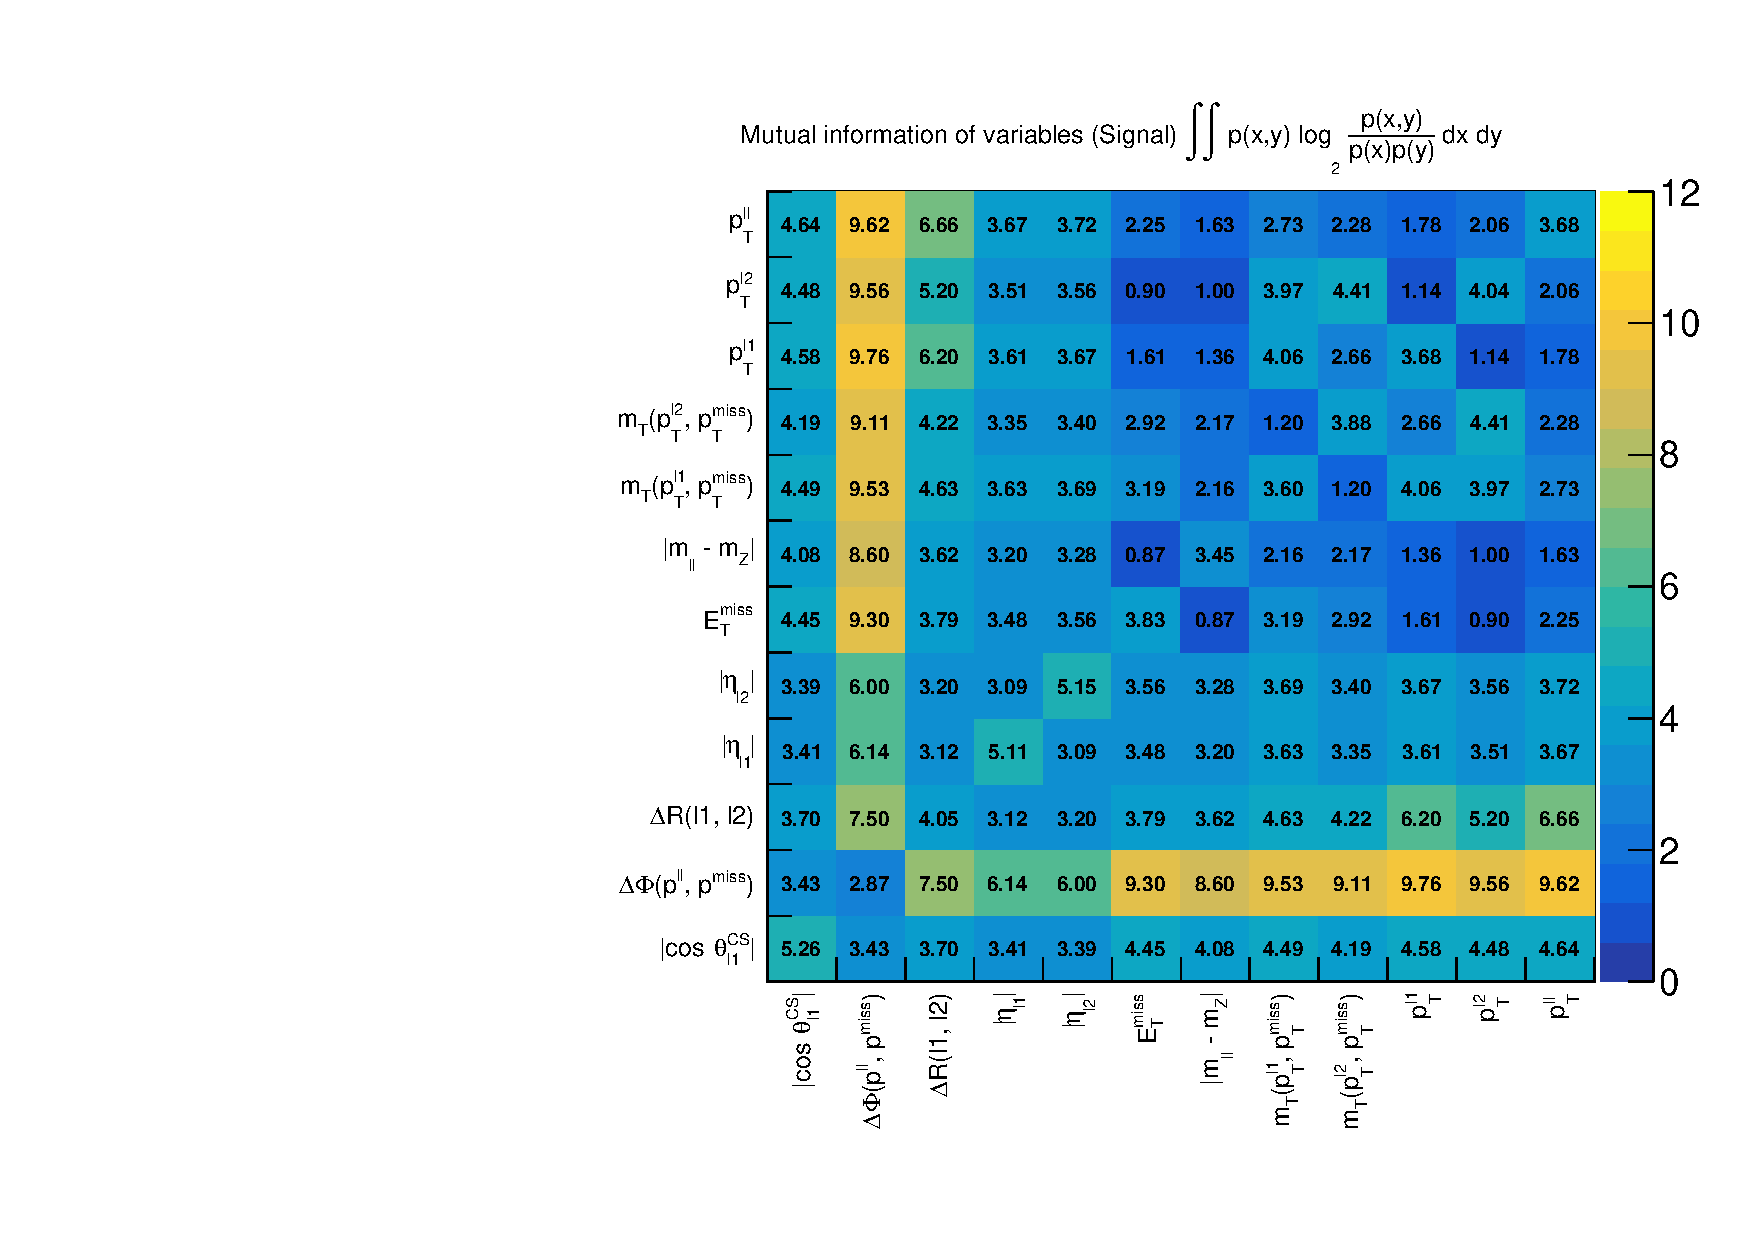
\includegraphics[width=0.48\textwidth]{figures/mutual_information_MVAvars_Signal.pdf}
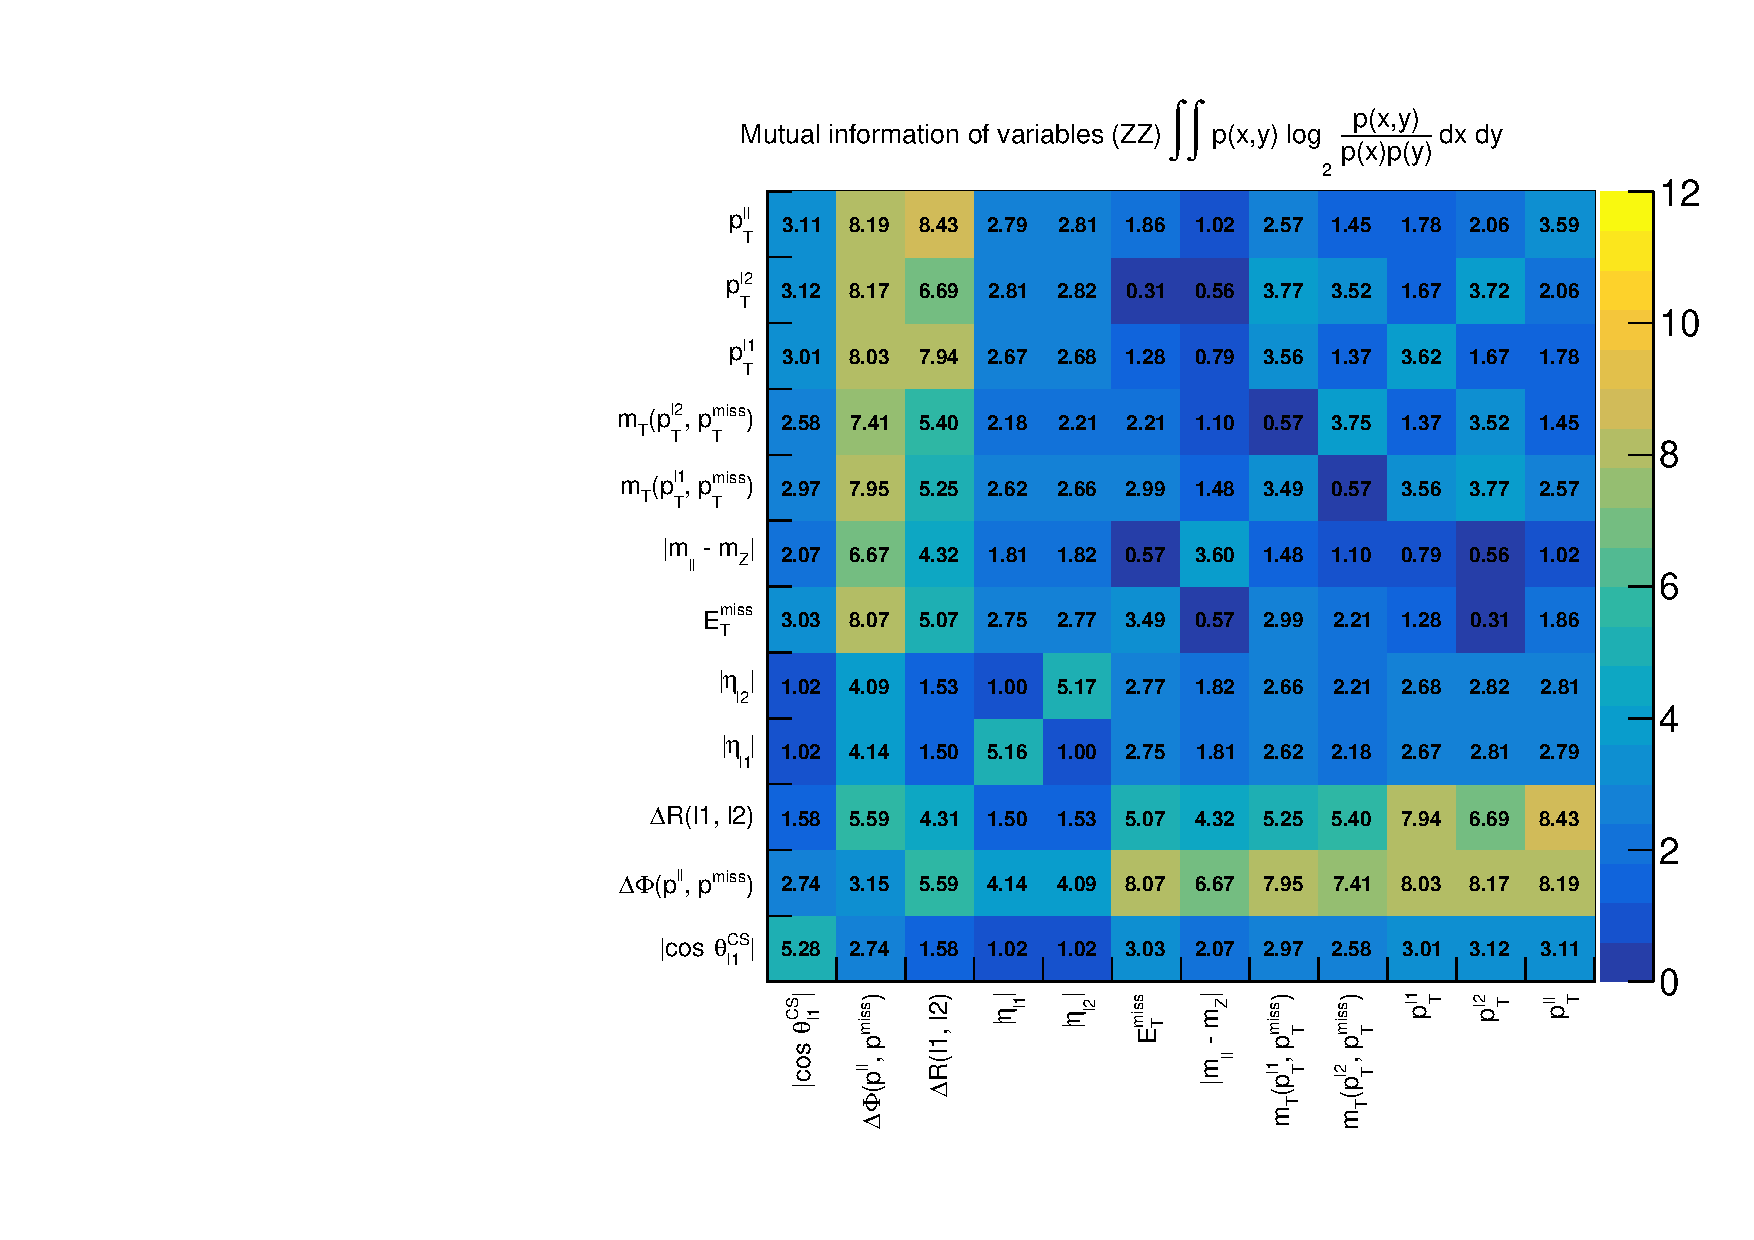
\includegraphics[width=0.48\textwidth]{figures/mutual_information_MVAvars_ZZ.pdf}
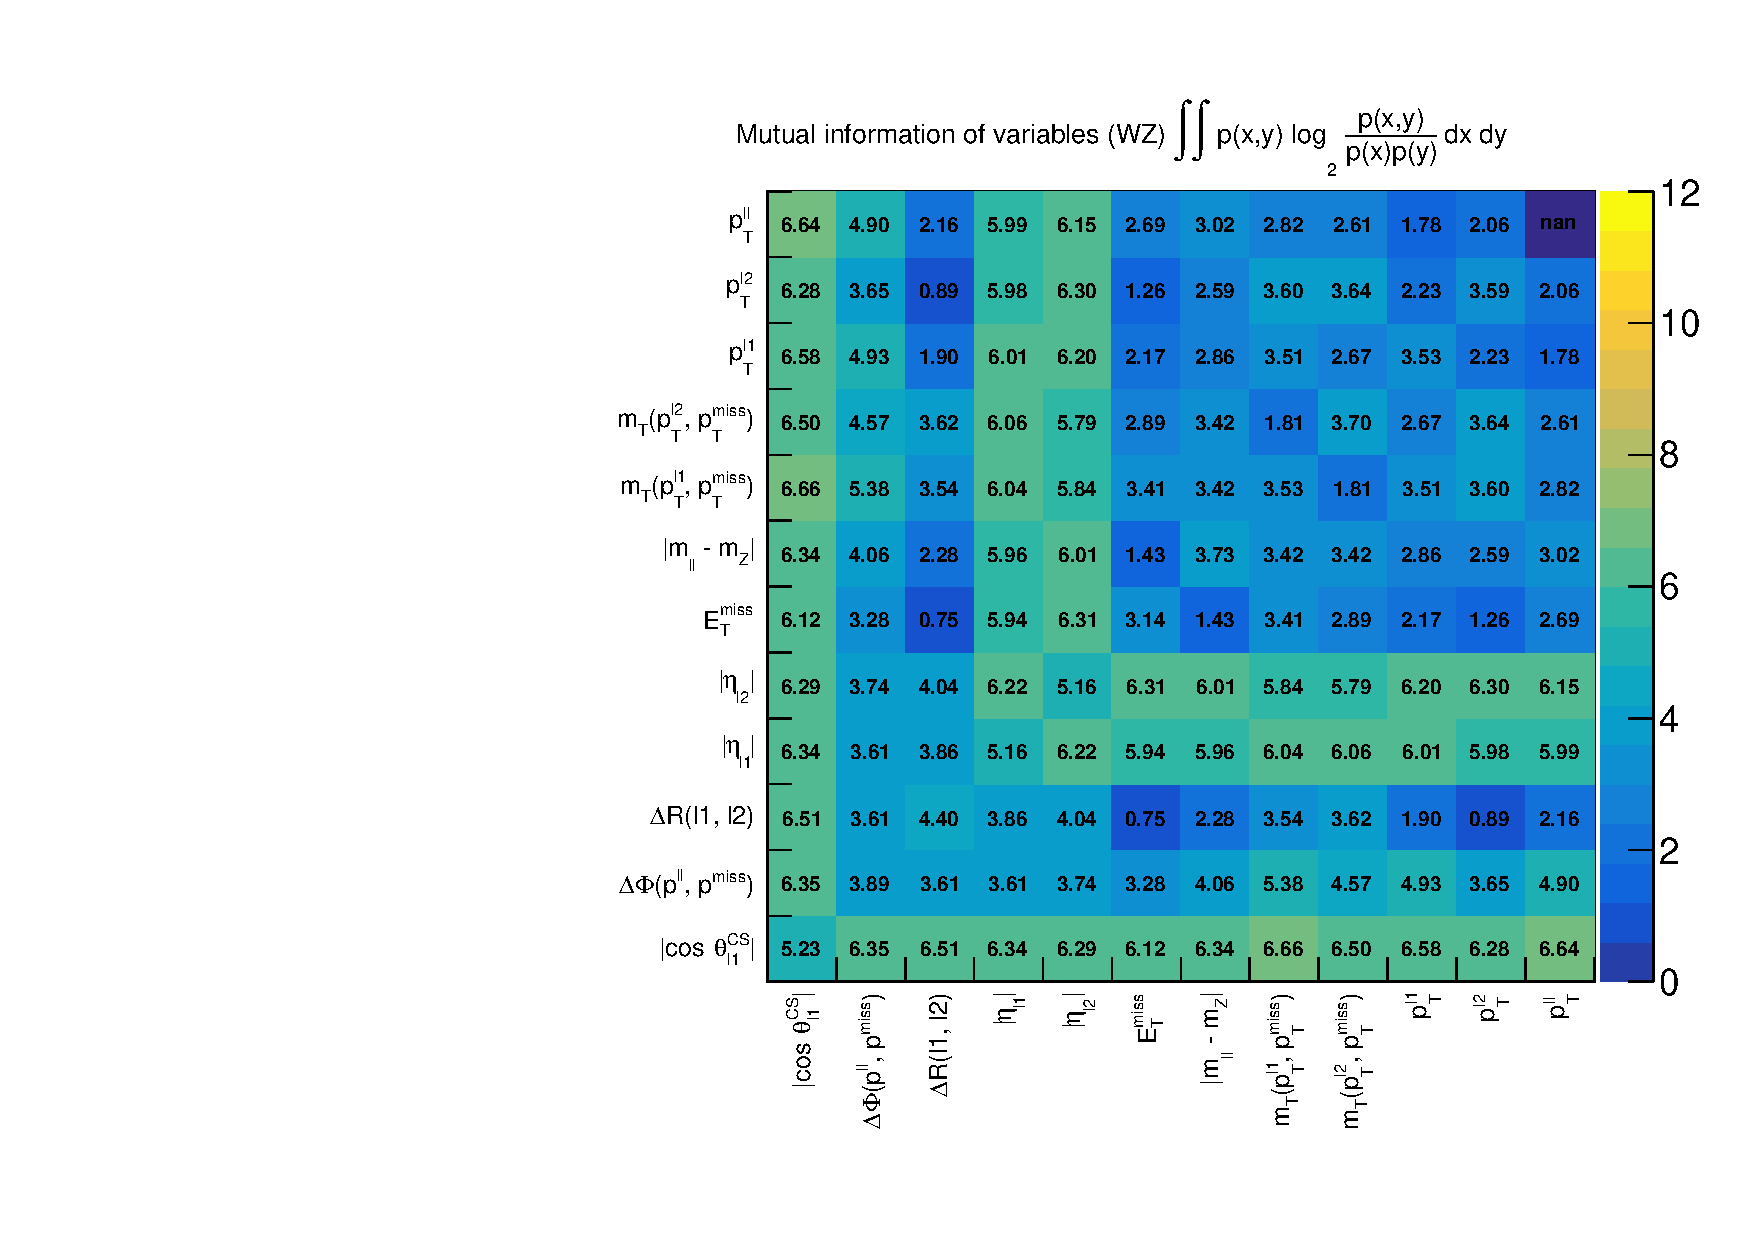
\includegraphics[width=0.48\textwidth]{figures/mutual_information_MVAvars_WZ.pdf}
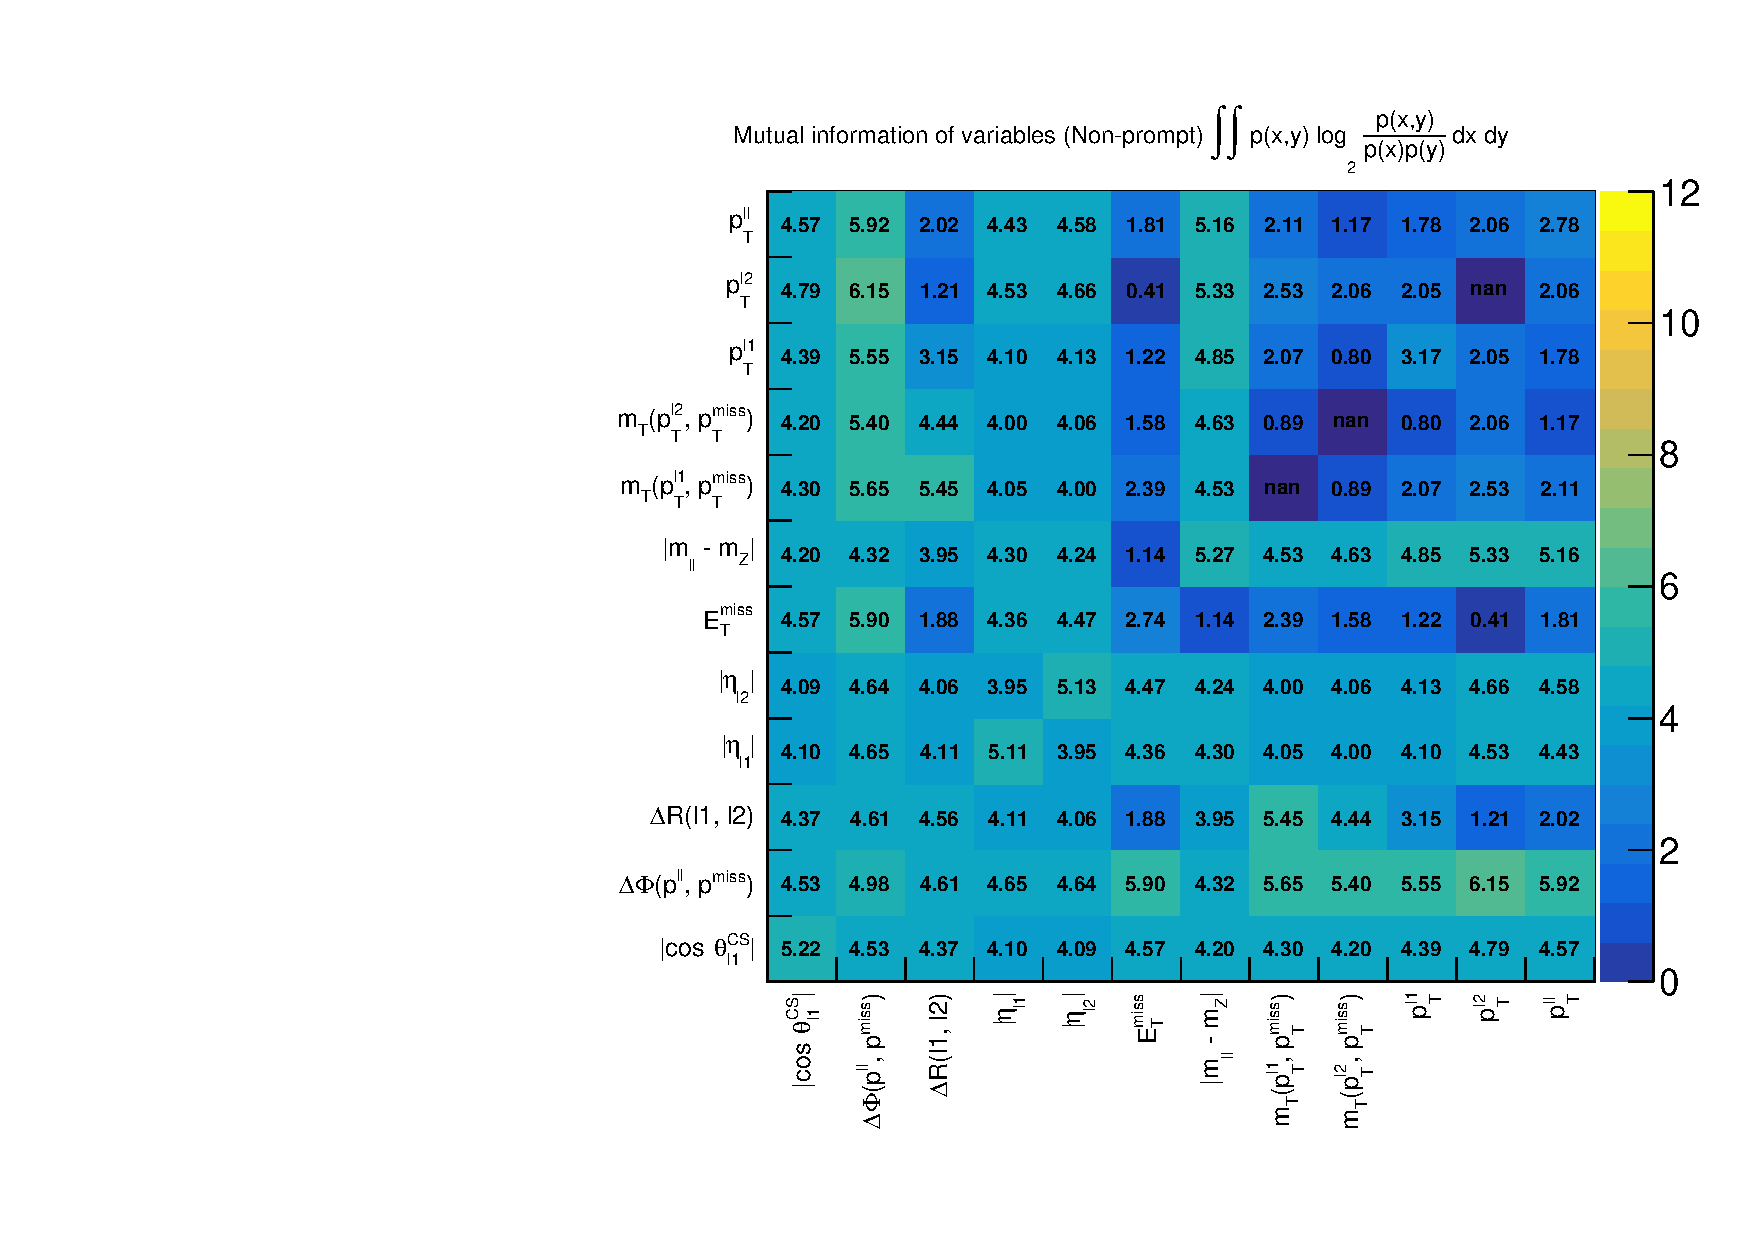
\includegraphics[width=0.48\textwidth]{figures/mutual_information_MVAvars_Non-prompt.pdf}
\caption{Mutual information between the twelve BDT input variables for the invisible Higgs, ZZ, WZ, and flavor-symmetric (non-prompt) classes. The matrix for the Drell-Yan class is statistically irrelevant.}
\label{fig:bdt_mutual_information}
\end{center}
\end{figure}

\begin{figure}[htbp]
\begin{center}
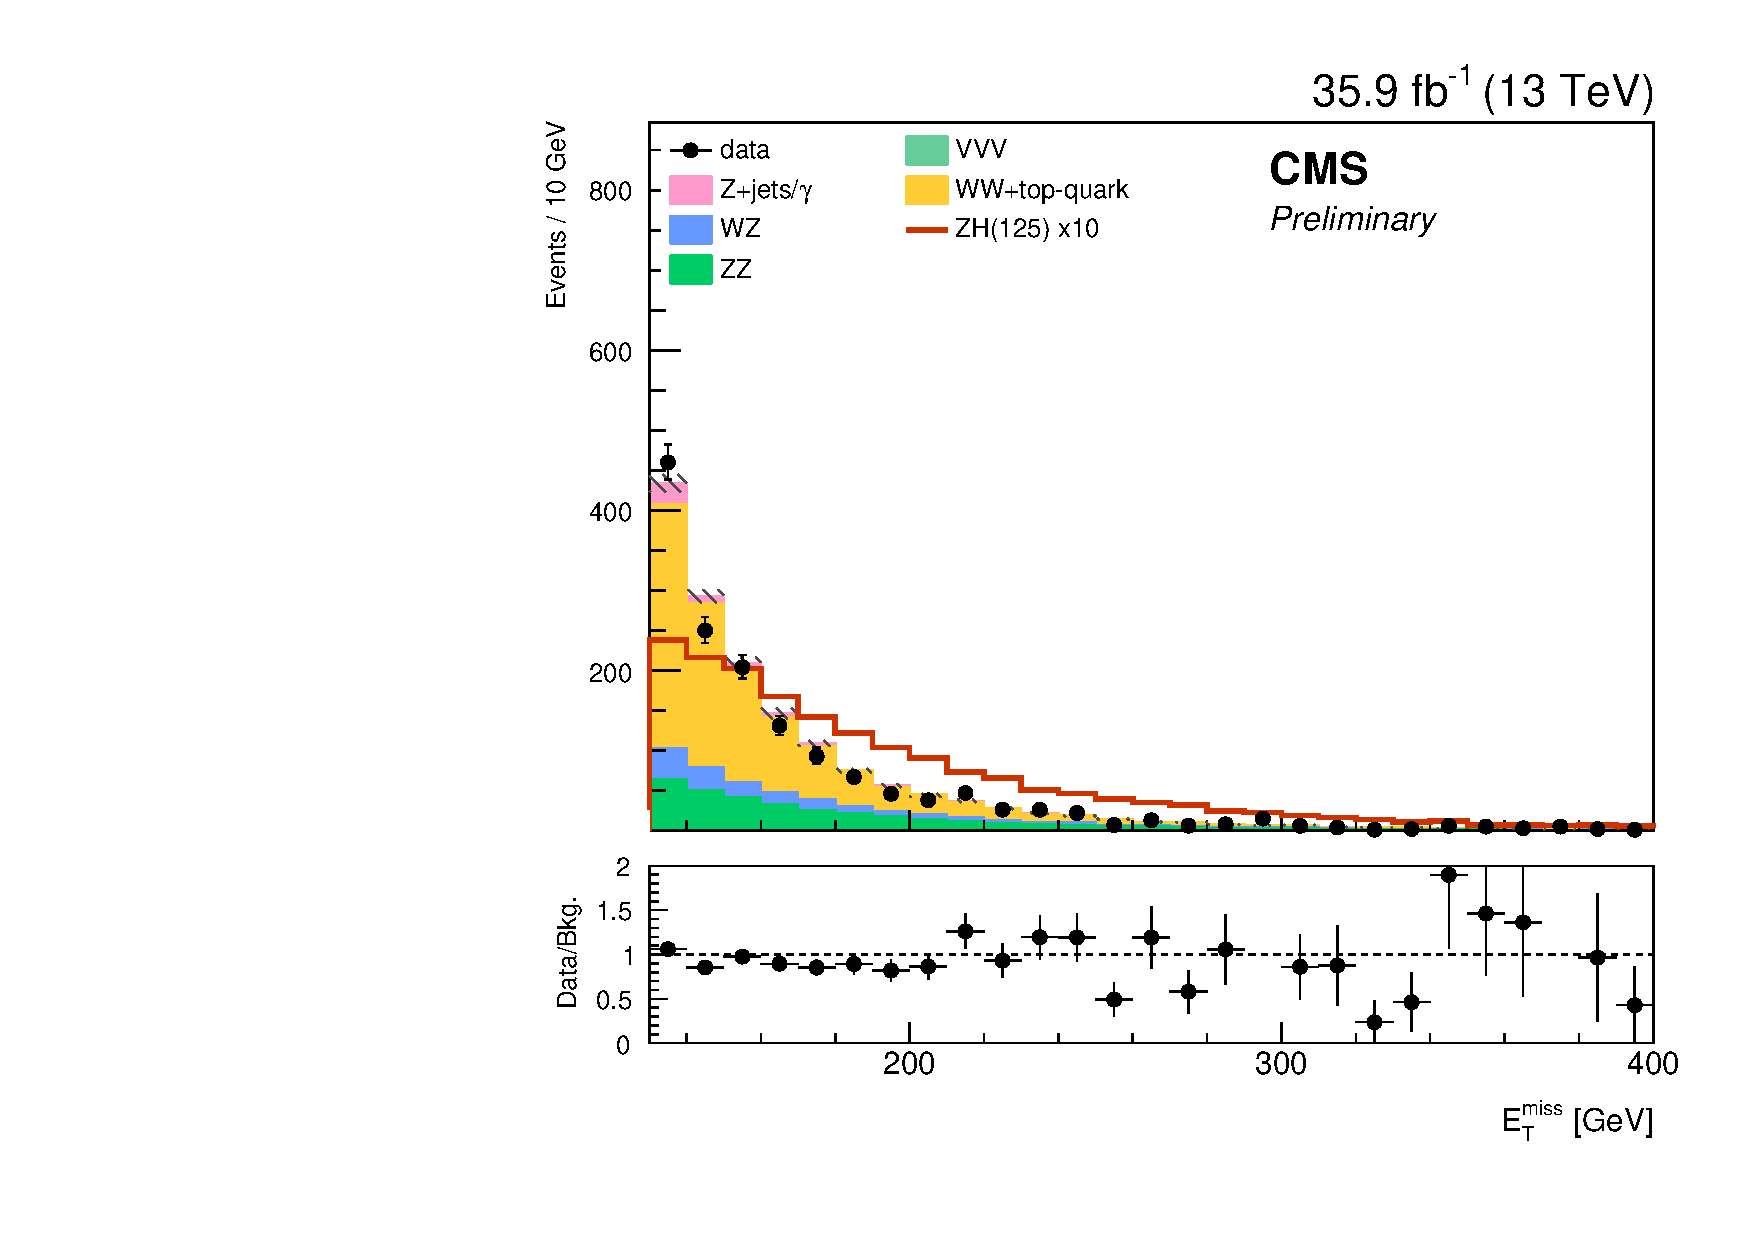
\includegraphics[width=0.48\textwidth]{figures/mva_MET_nice.pdf}
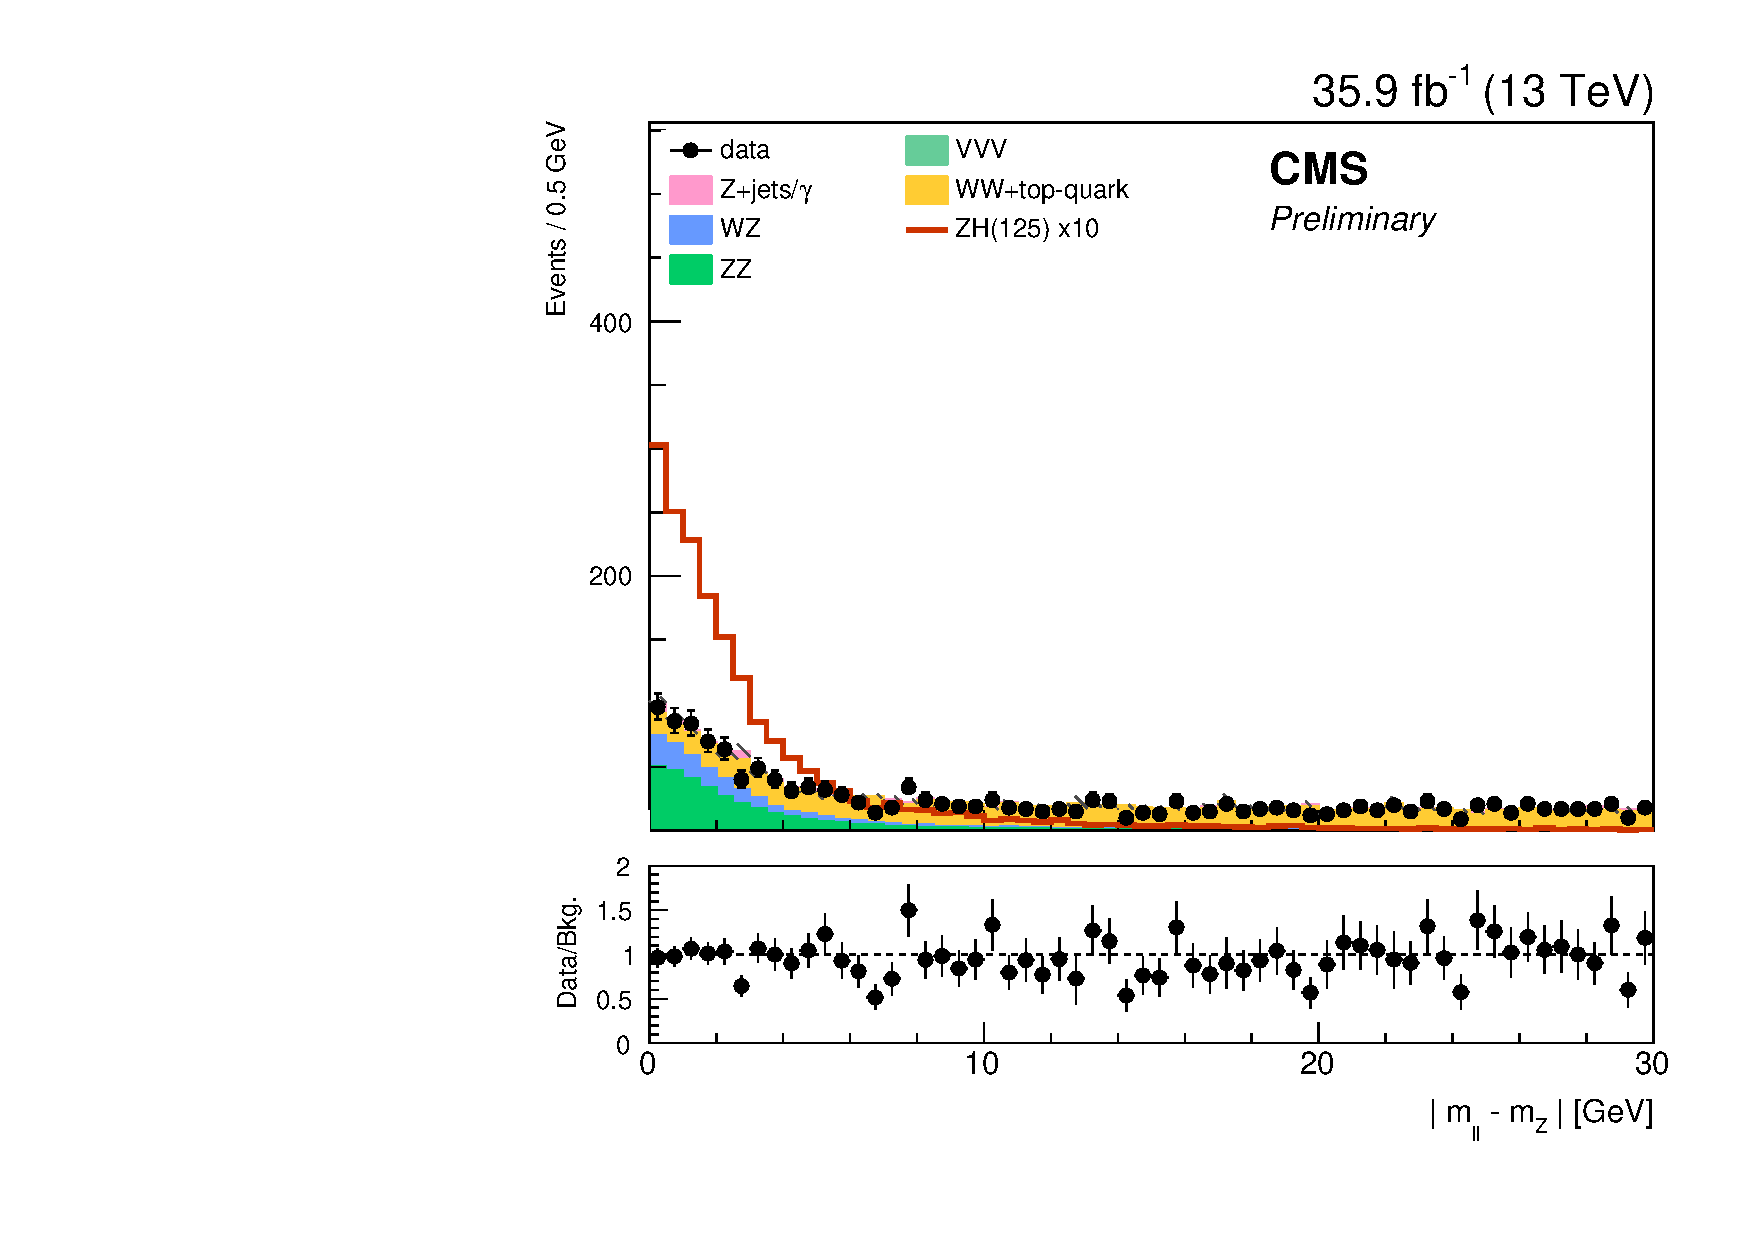
\includegraphics[width=0.48\textwidth]{figures/mva_mll_minus_mZ_nice.pdf}
%\includegraphics[width=0.48\textwidth]{figures/mva_balance_nice.pdf}
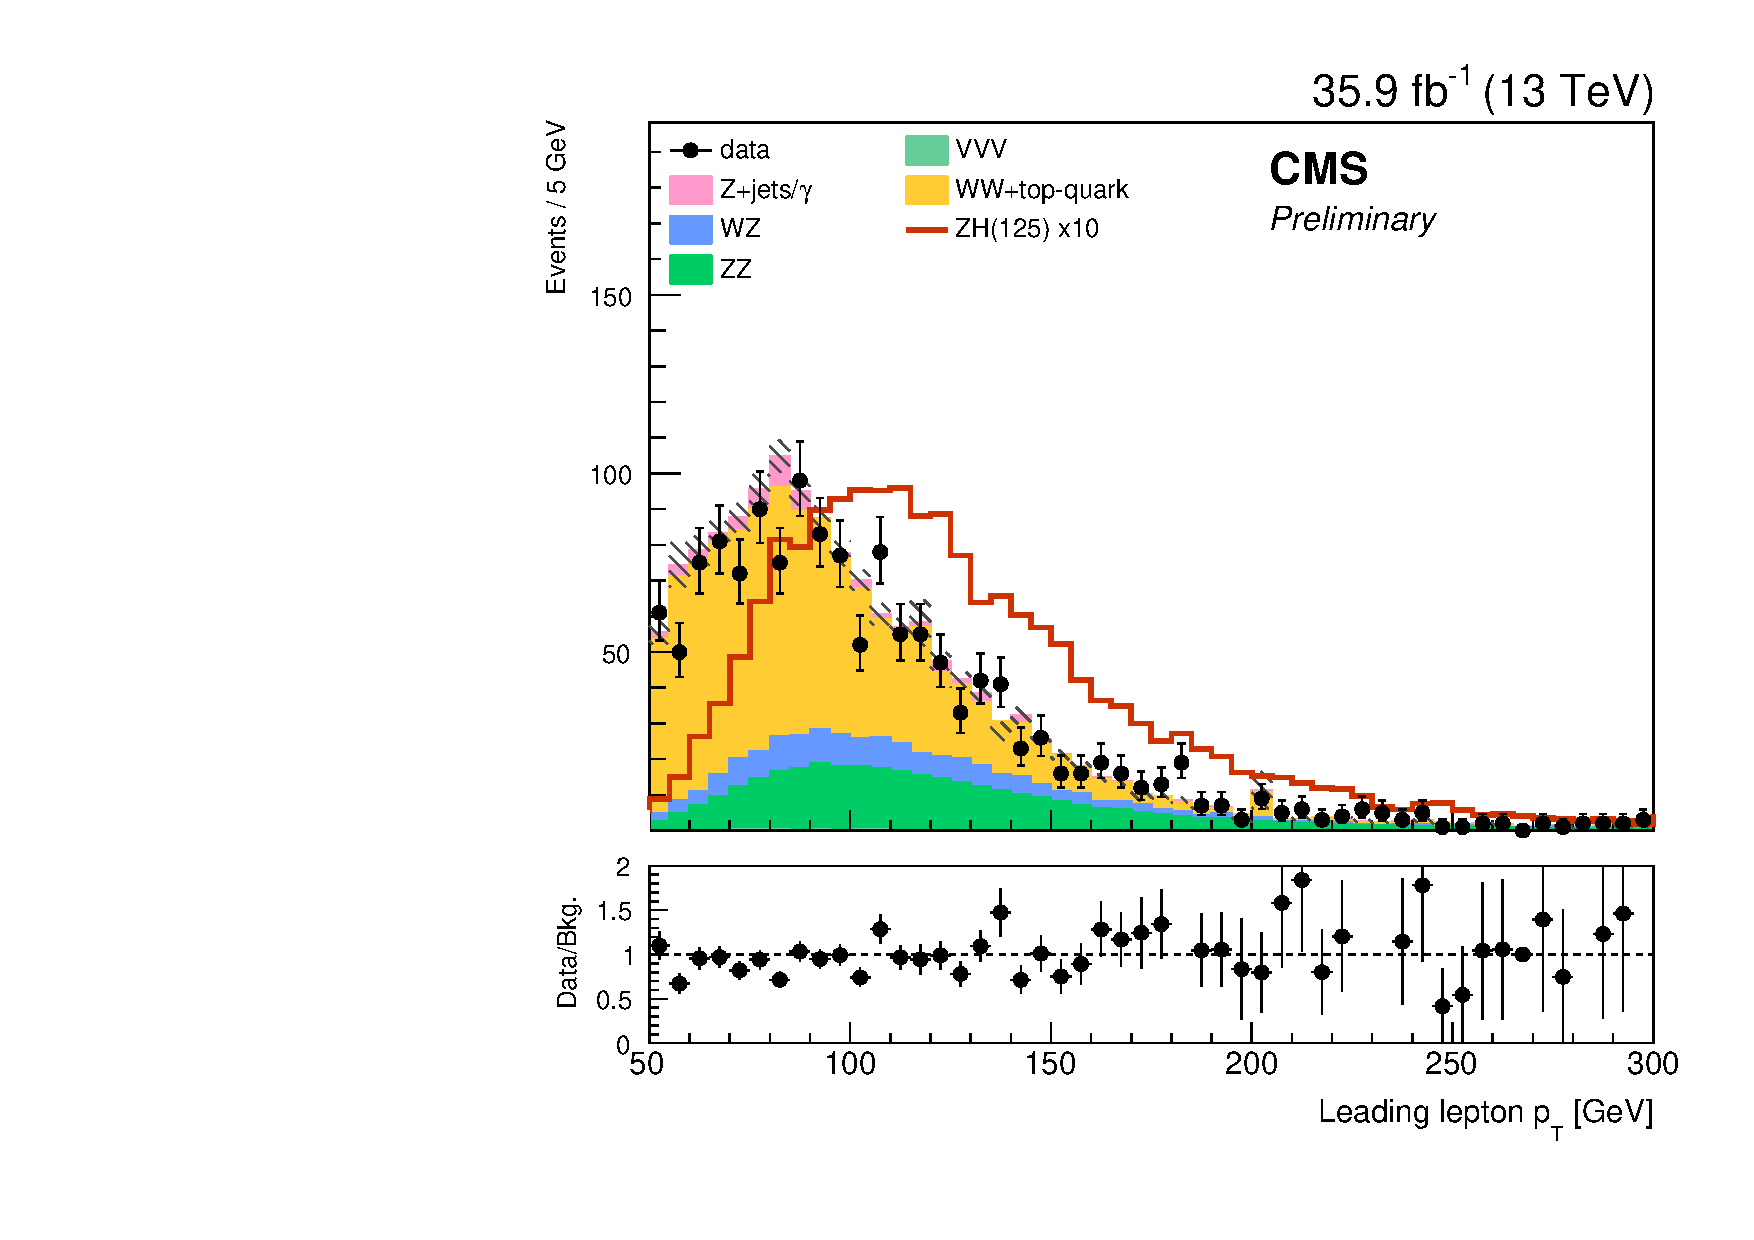
\includegraphics[width=0.48\textwidth]{figures/mva_ptl1_nice.pdf}
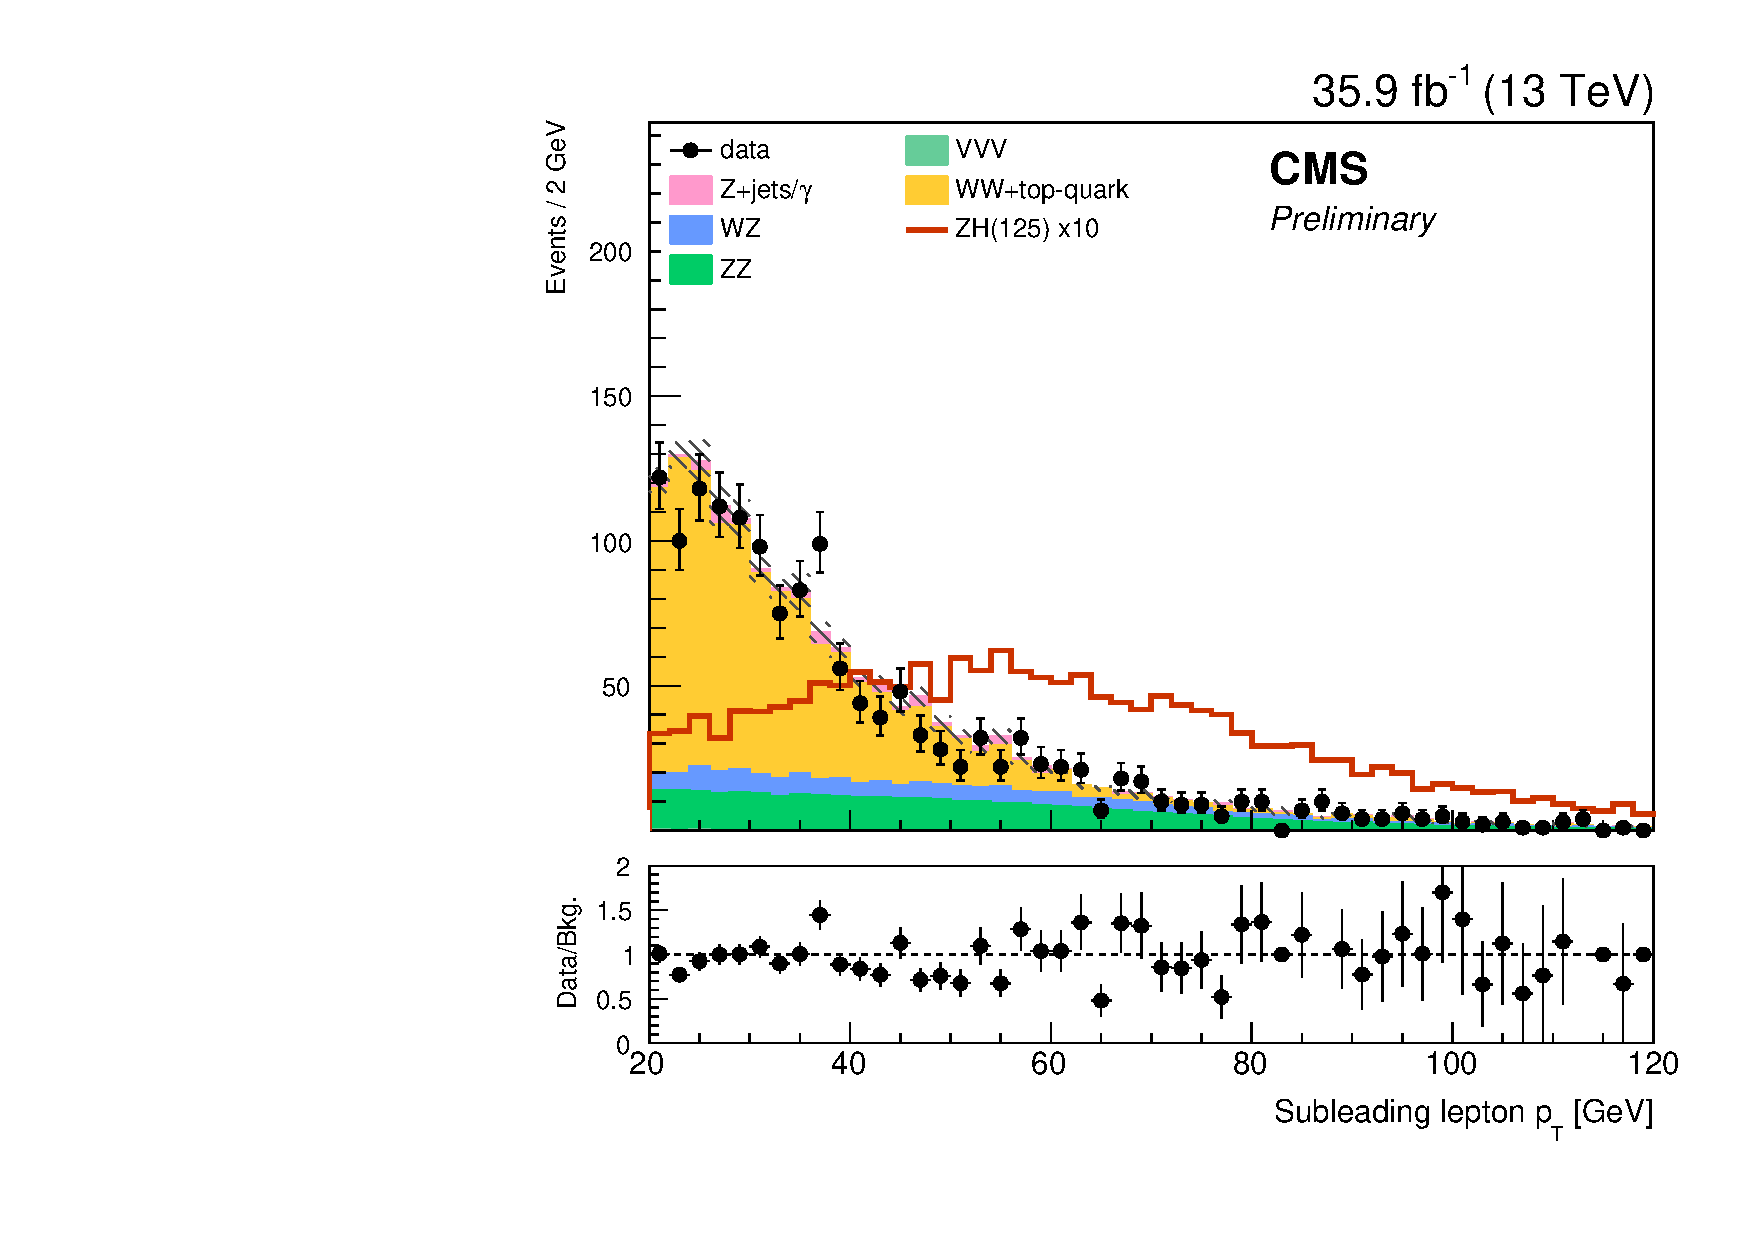
\includegraphics[width=0.48\textwidth]{figures/mva_ptl2_nice.pdf}
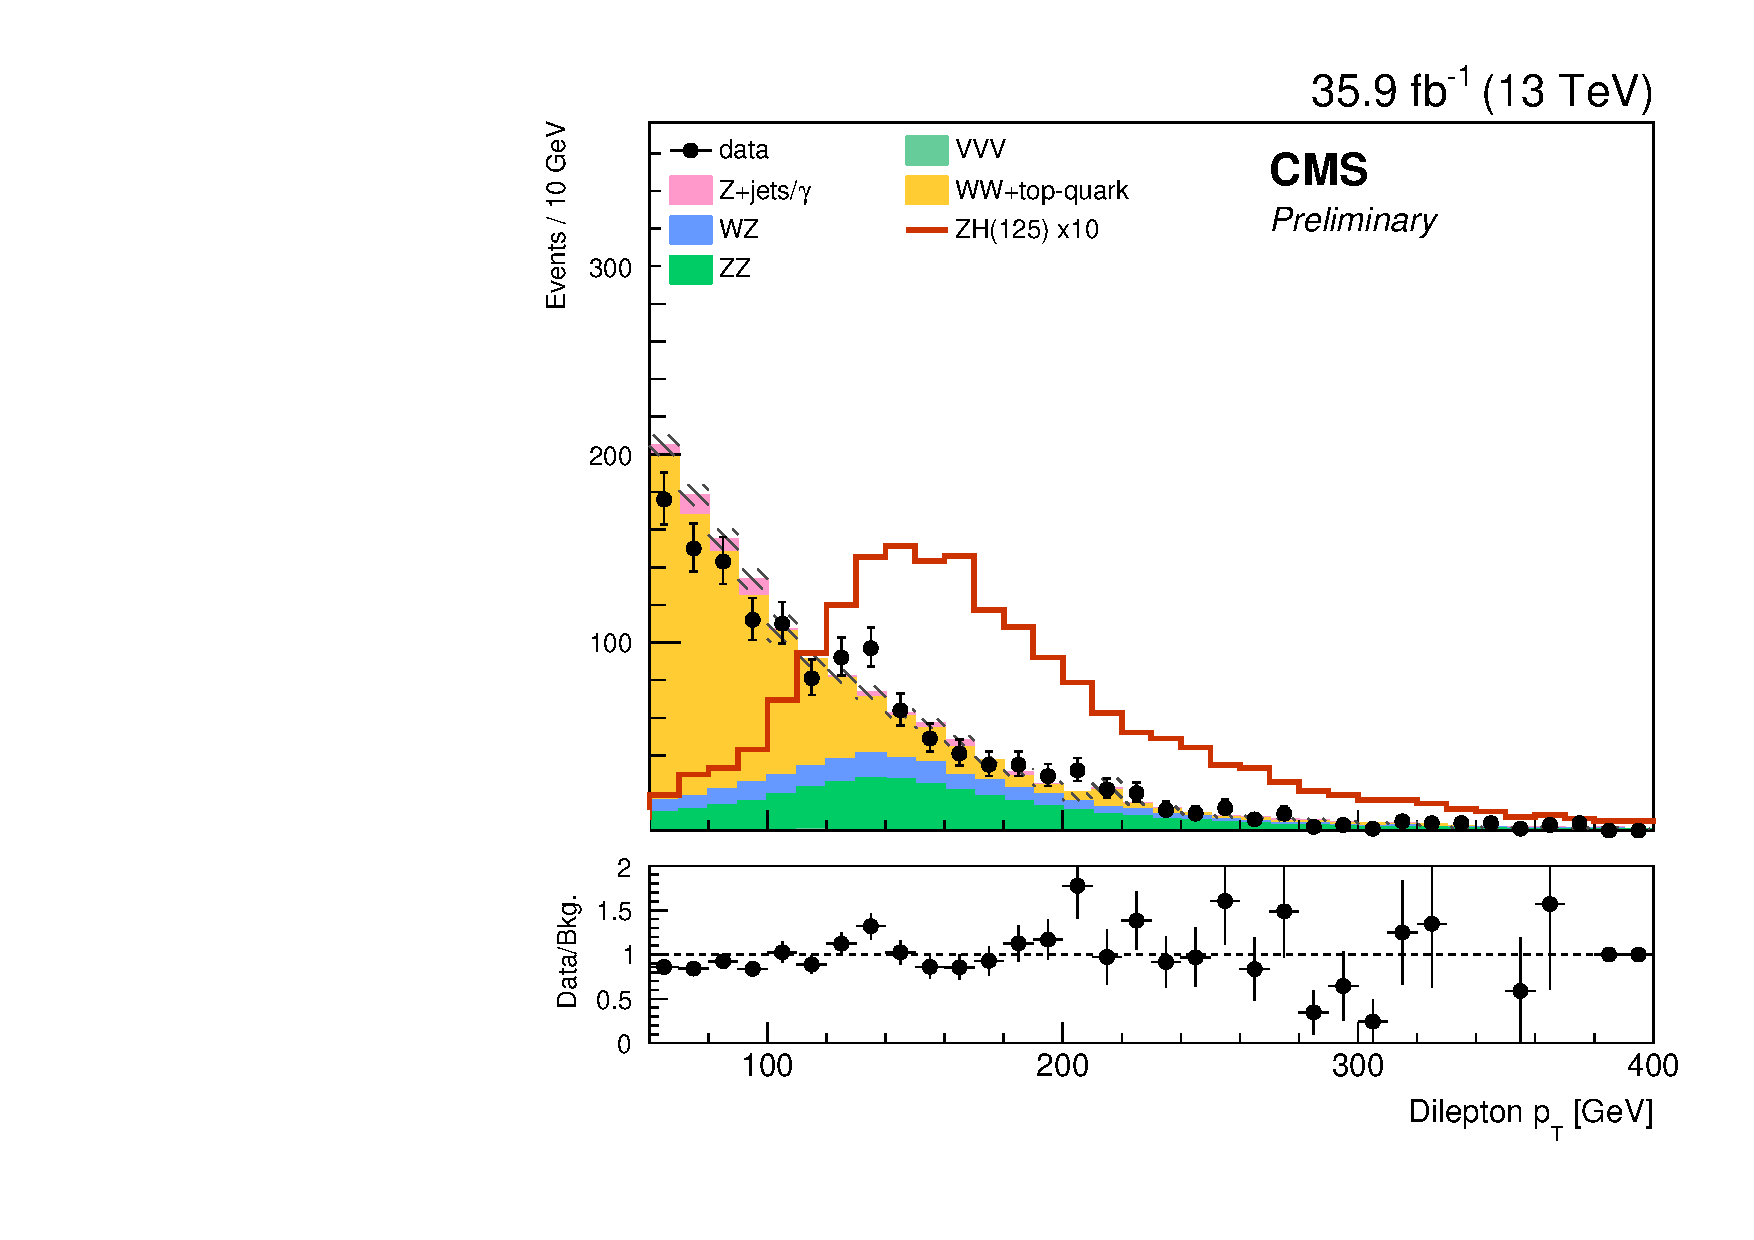
\includegraphics[width=0.48\textwidth]{figures/mva_ptll_nice.pdf}
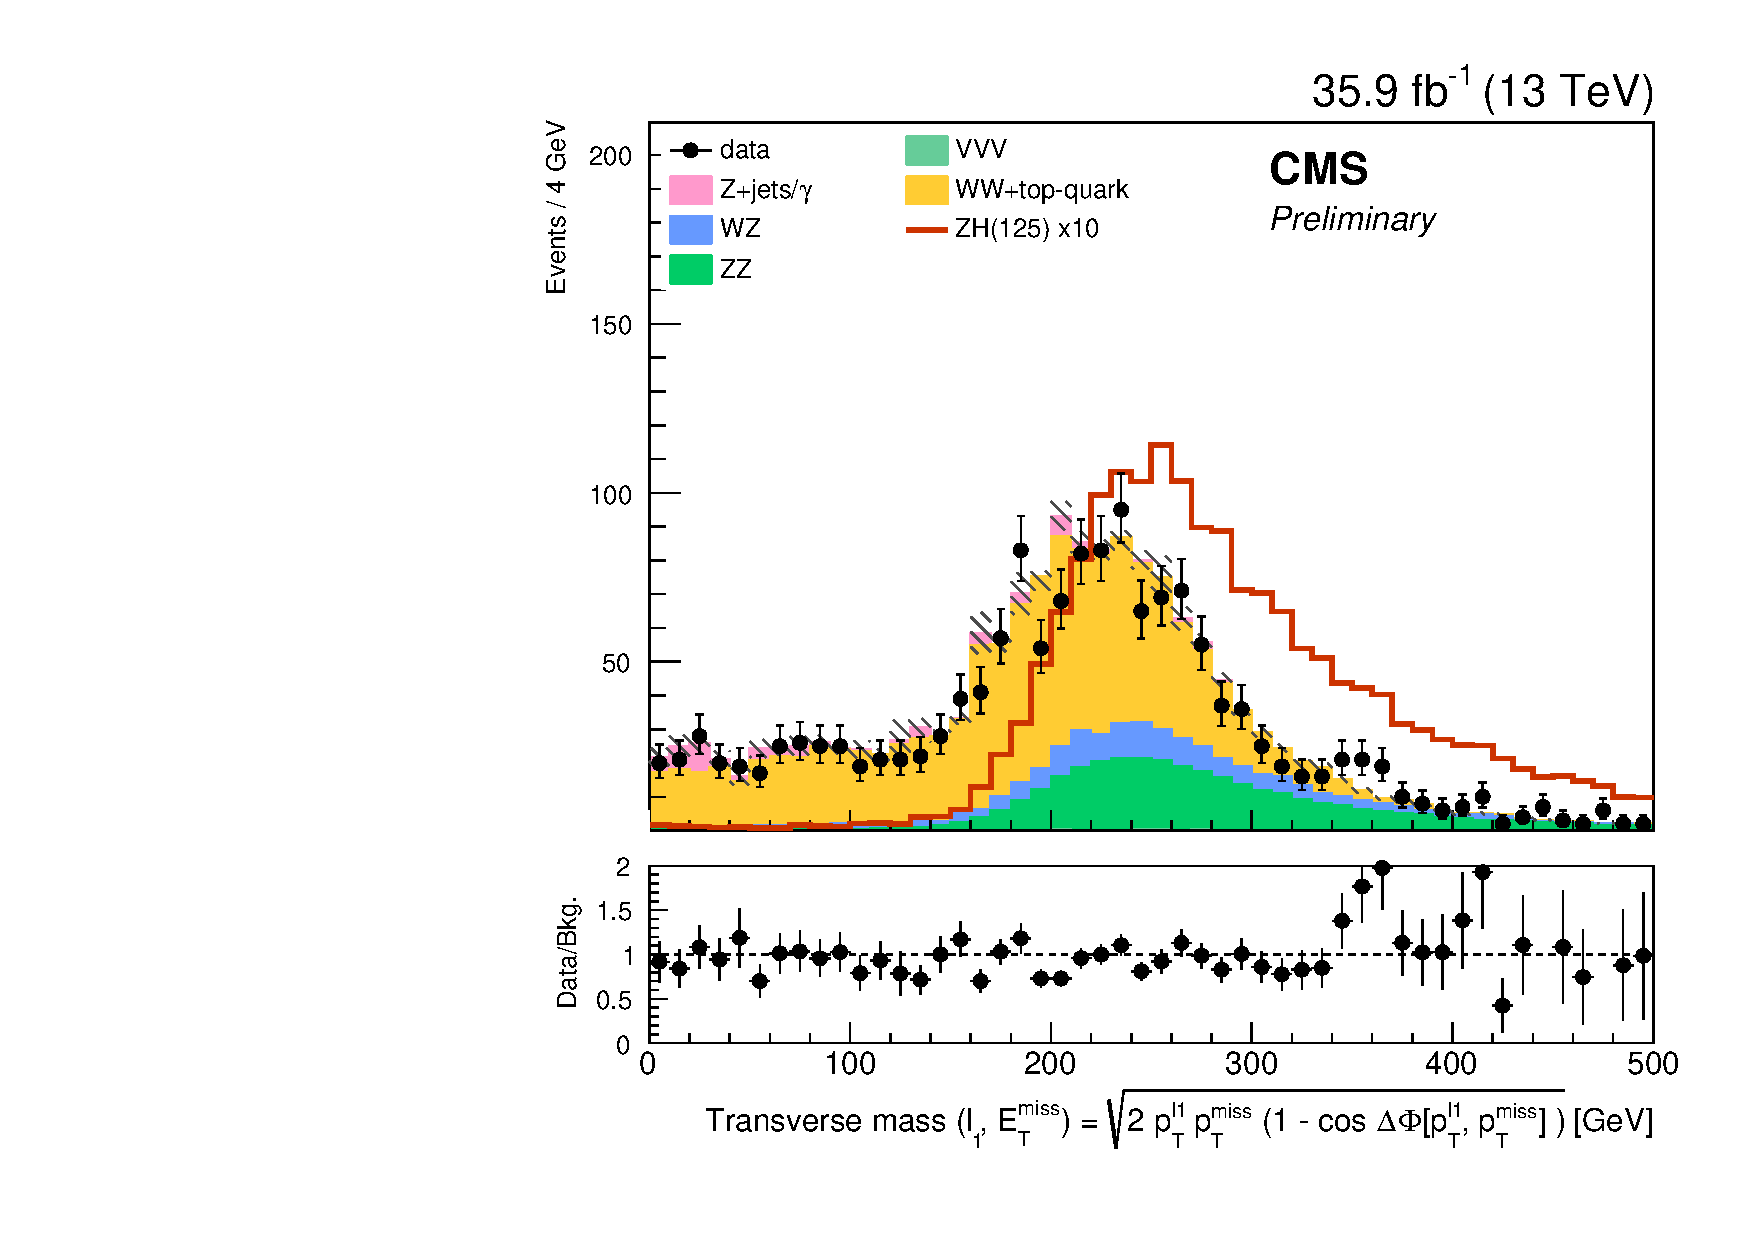
\includegraphics[width=0.48\textwidth]{figures/mva_mTl1MET_nice.pdf}
\caption{Comparison of data and prediction in the BDT input variables after applying the training preselection. Signal strength has been enhanced by a factor of 10.}
\label{fig:bdt_inputvar_histos}
\end{center}
\end{figure}
\begin{figure}[htbp]
\begin{center}
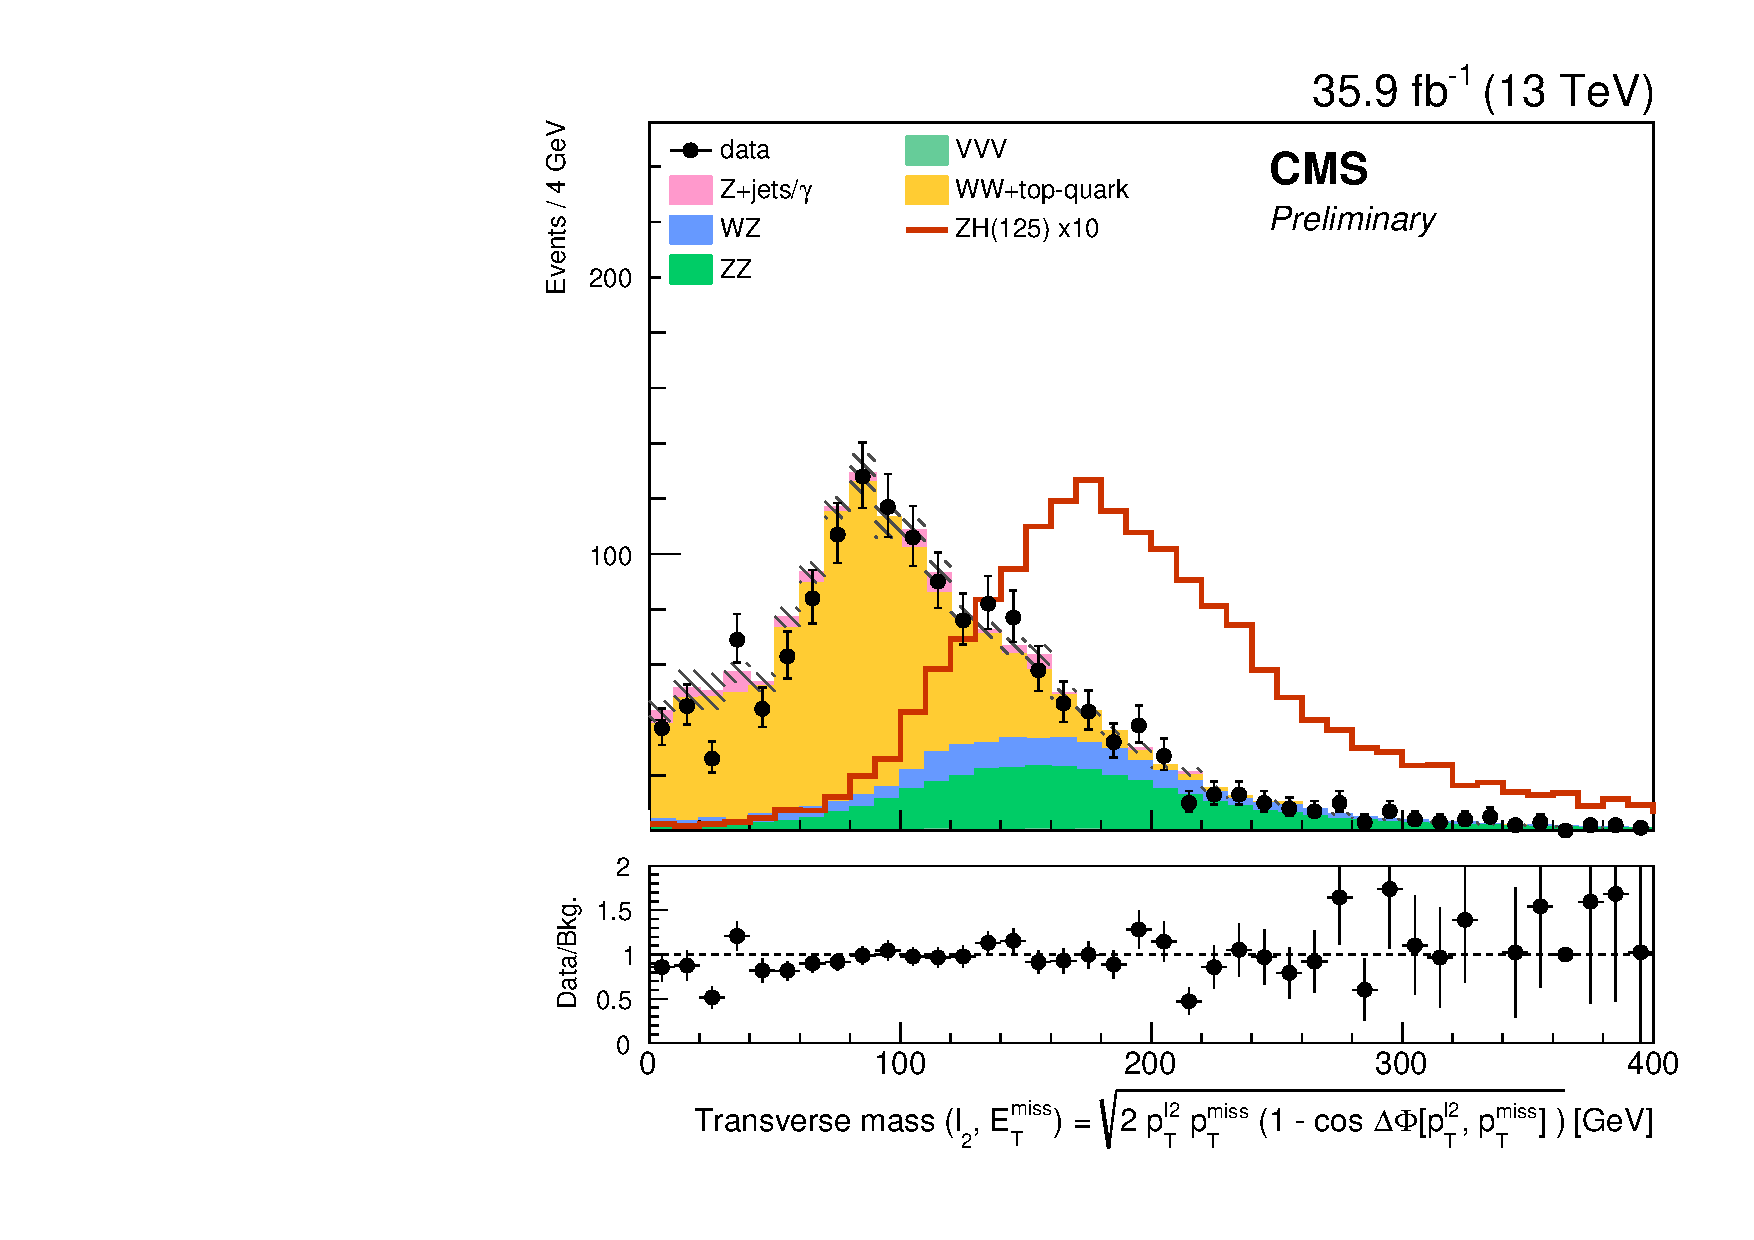
\includegraphics[width=0.48\textwidth]{figures/mva_mTl2MET_nice.pdf}
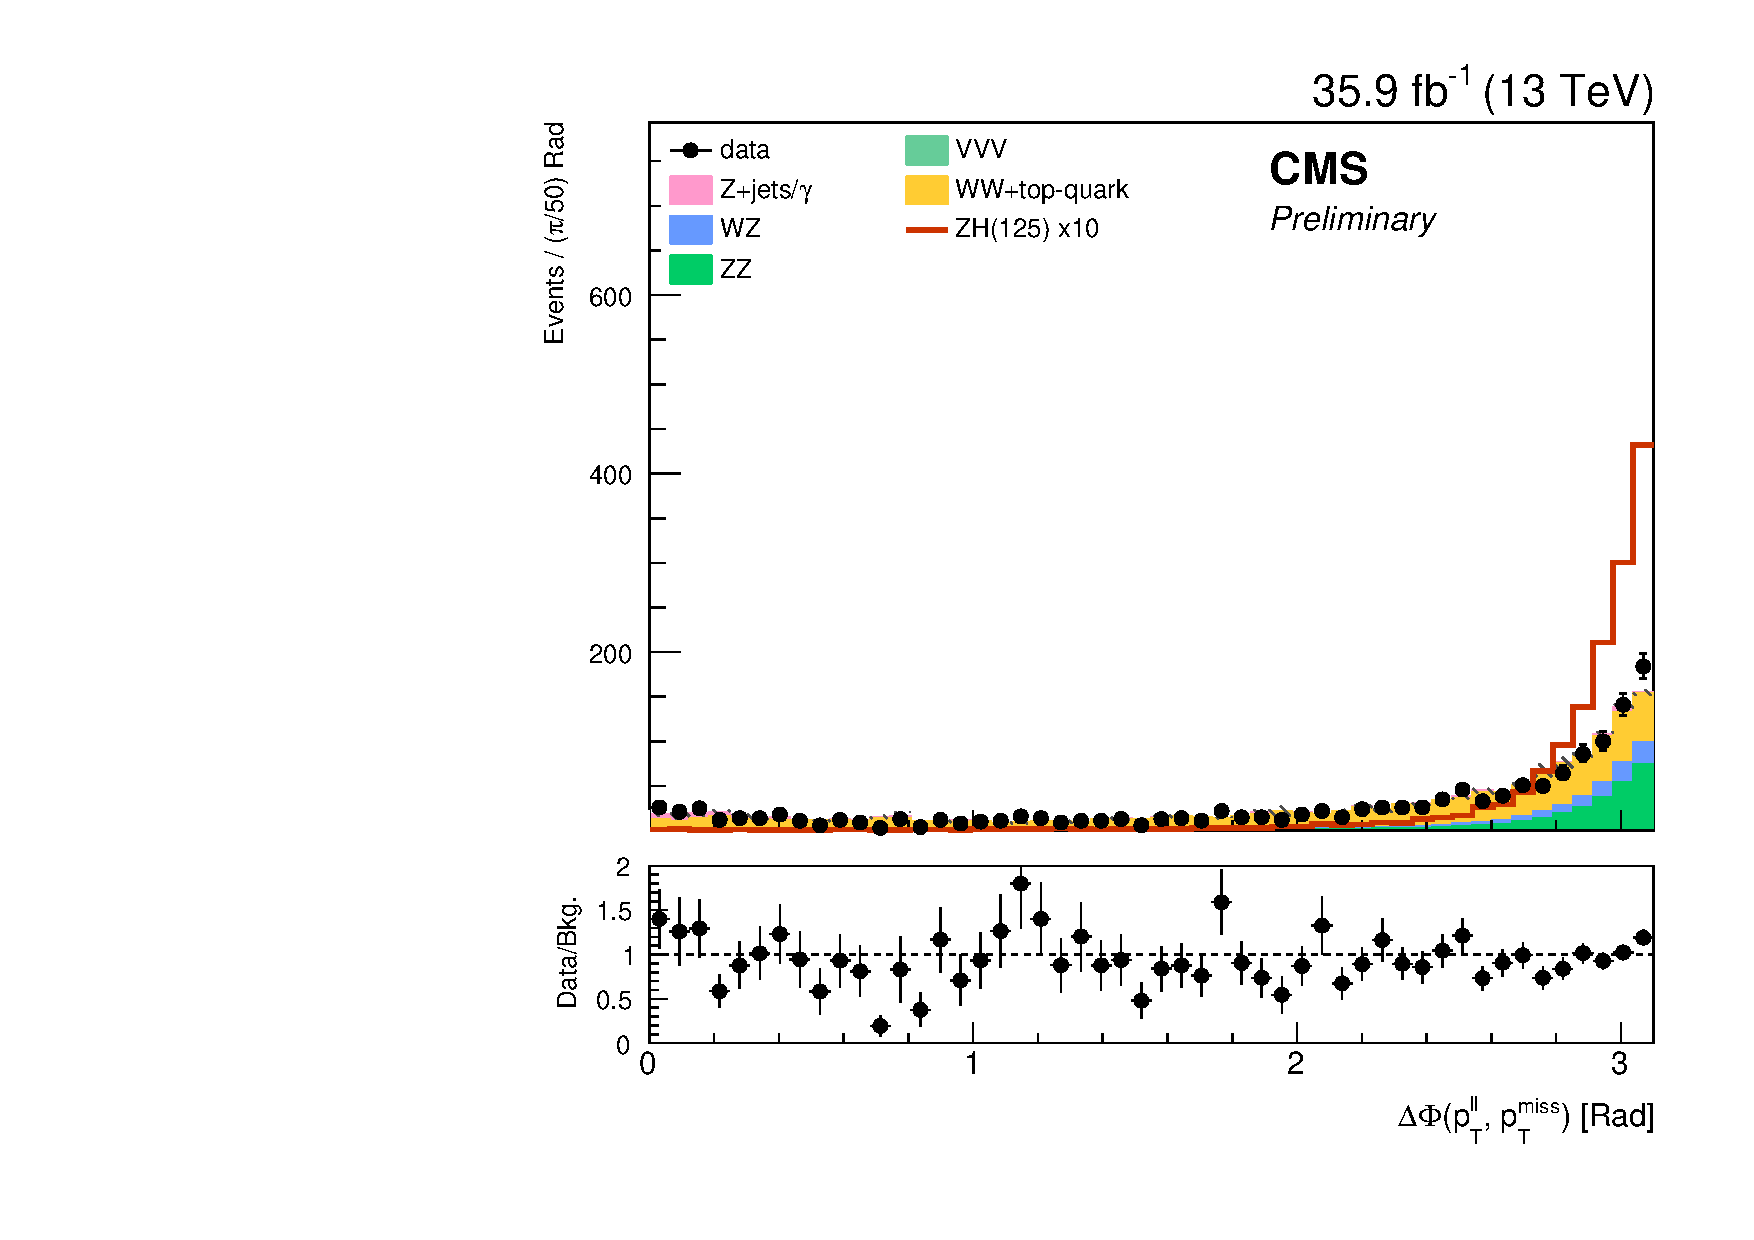
\includegraphics[width=0.48\textwidth]{figures/mva_delphi_ptll_MET_nice.pdf}
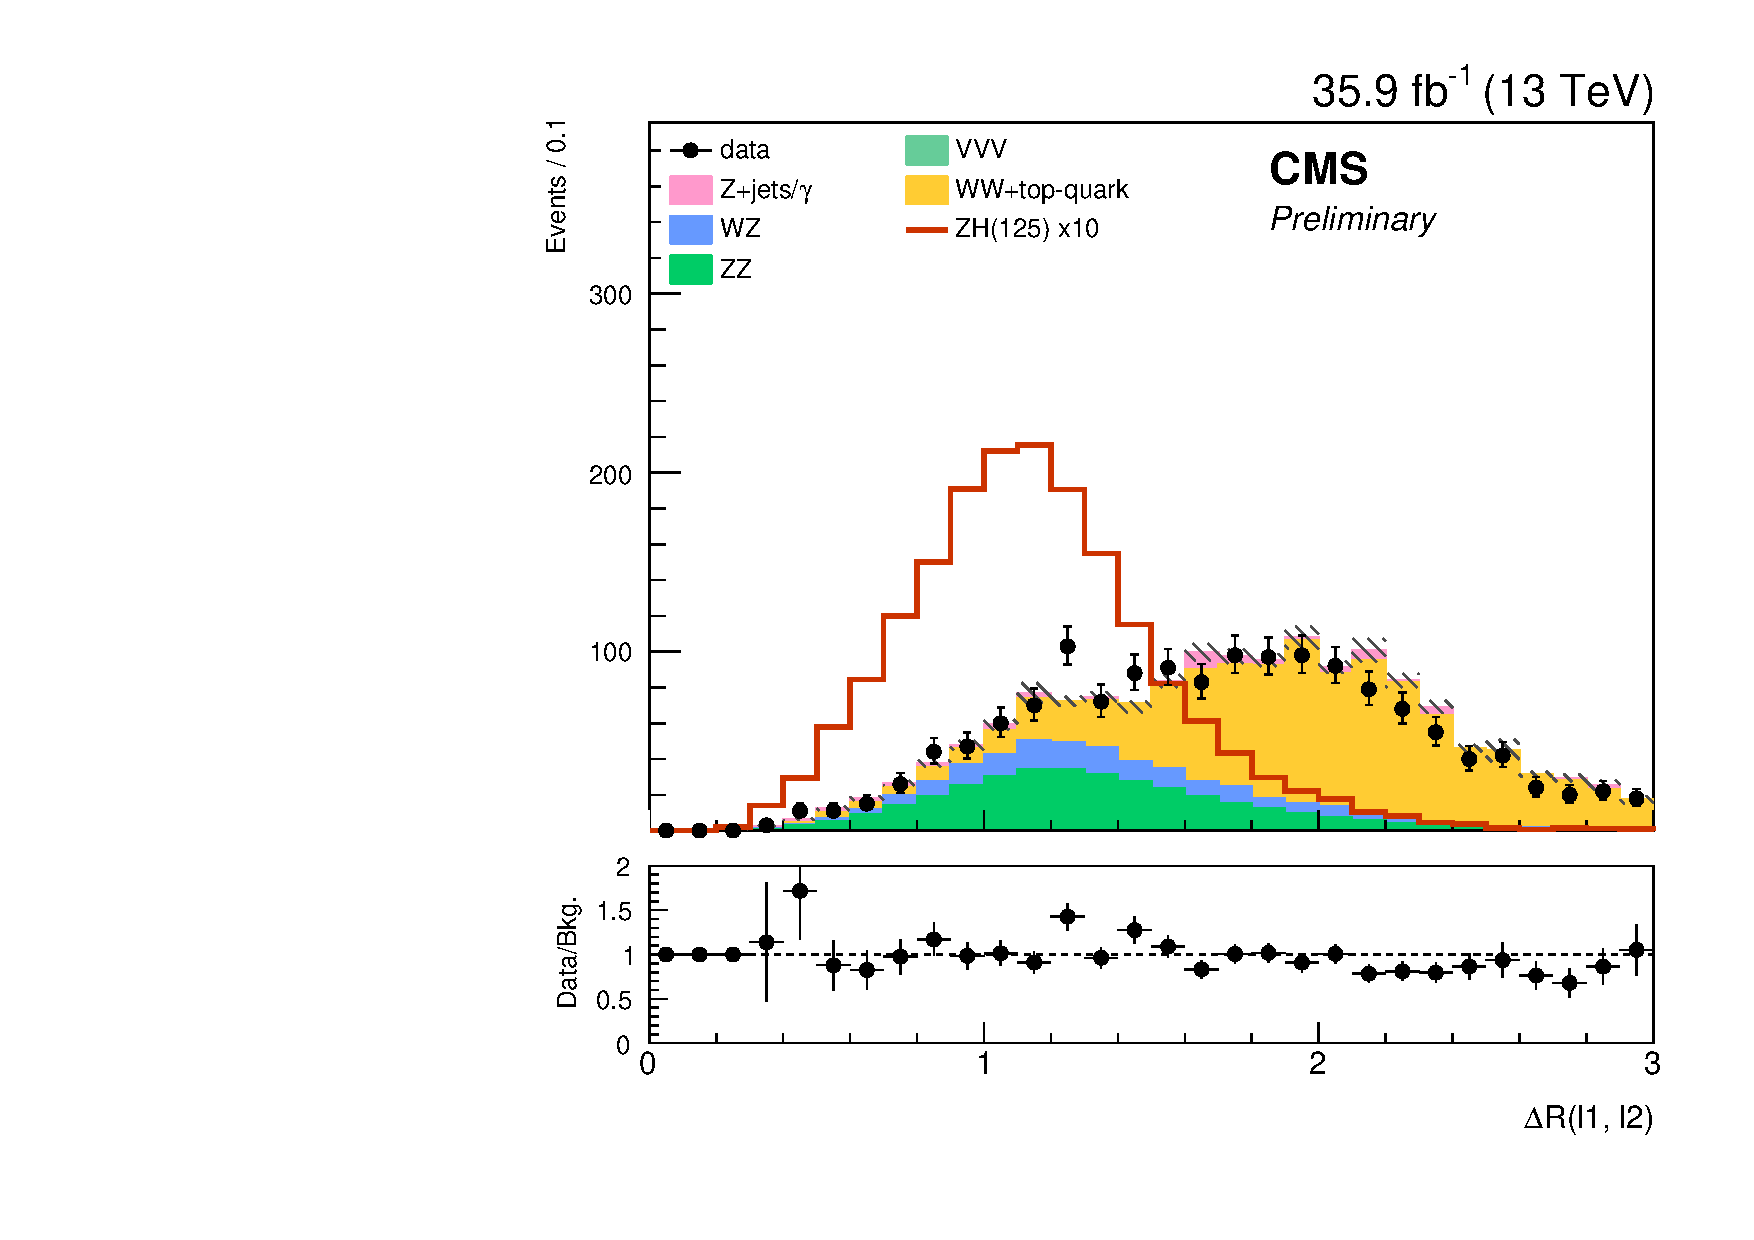
\includegraphics[width=0.48\textwidth]{figures/mva_deltaR_ll_nice.pdf}
%\includegraphics[width=0.48\textwidth]{figures/mva_ptl1mptl2_over_ptll_nice.pdf}
%\includegraphics[width=0.48\textwidth]{figures/mva_cos_theta_star_l1_nice.pdf}
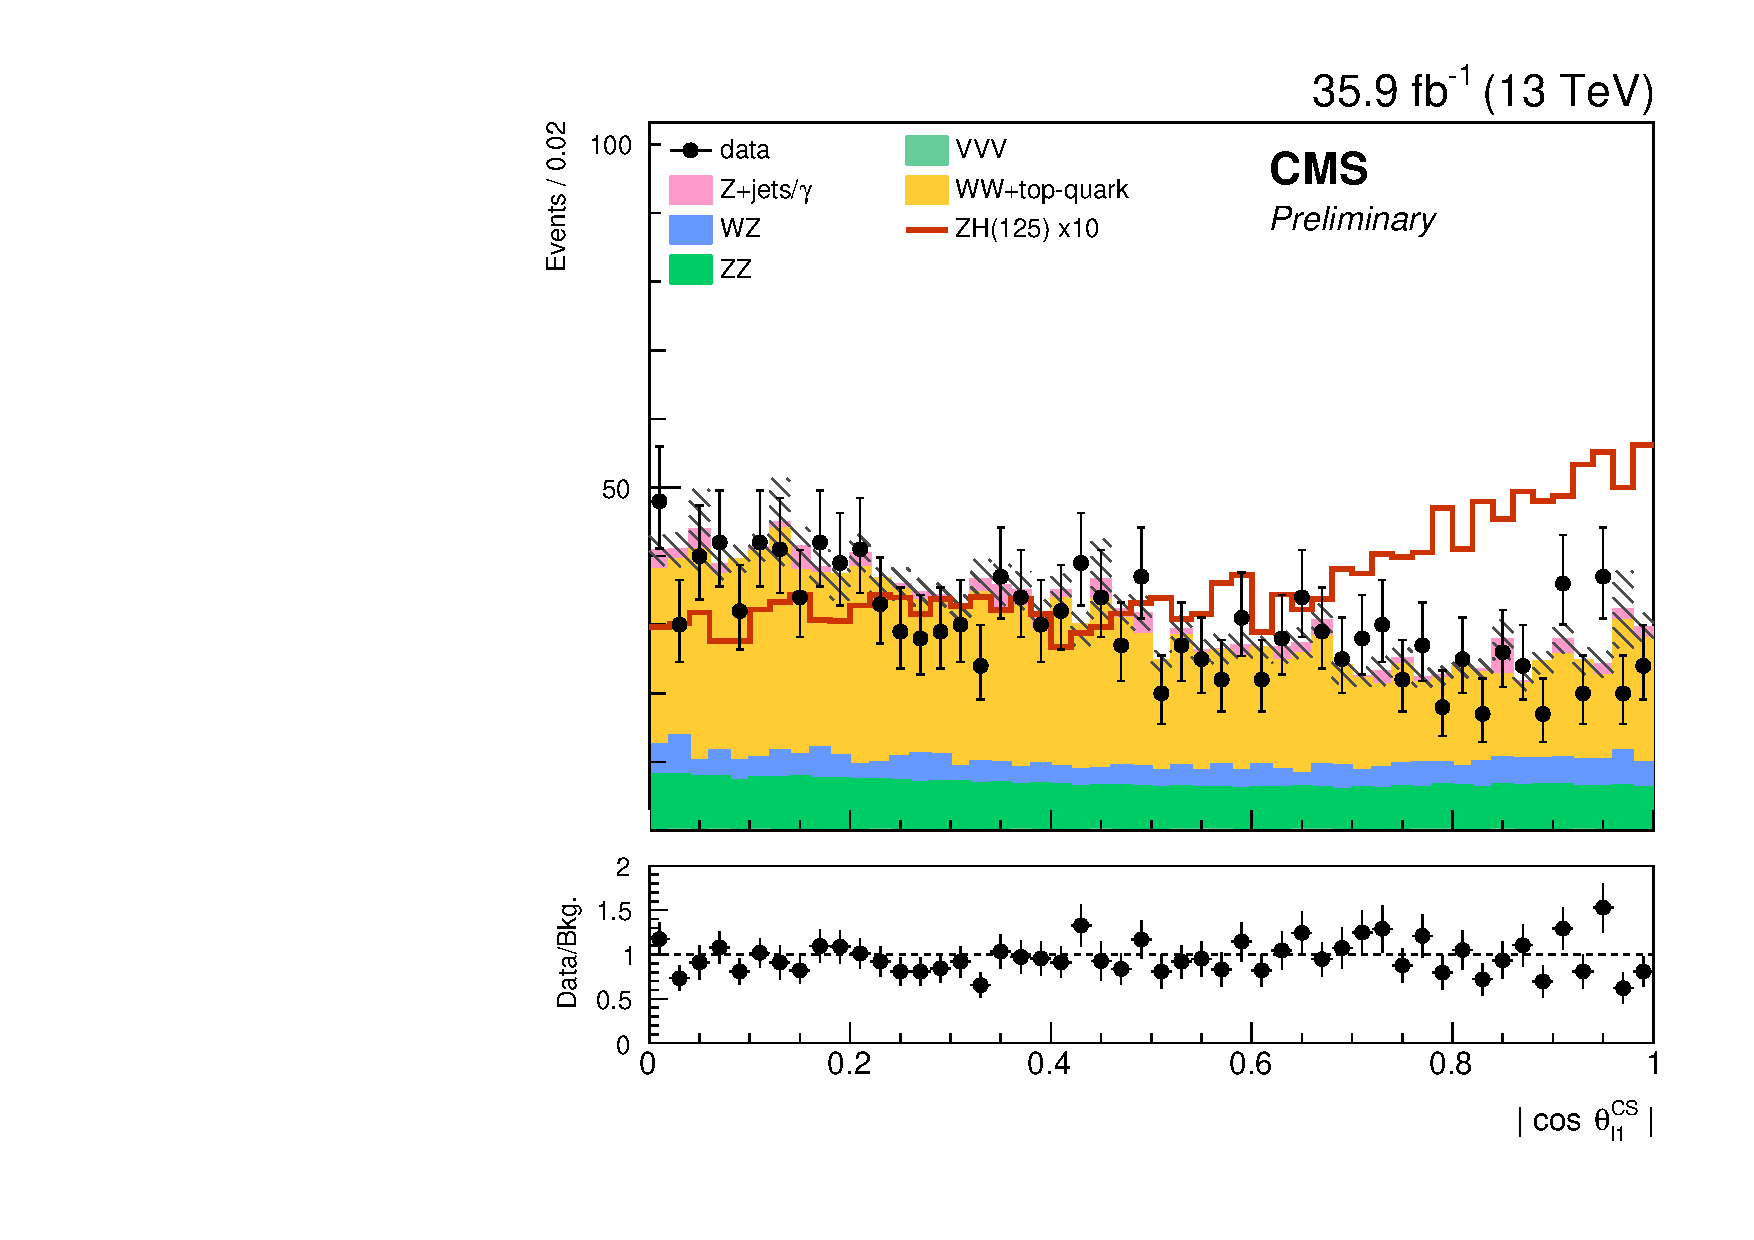
\includegraphics[width=0.48\textwidth]{figures/mva_abs_cos_theta_CS_l1_nice.pdf}
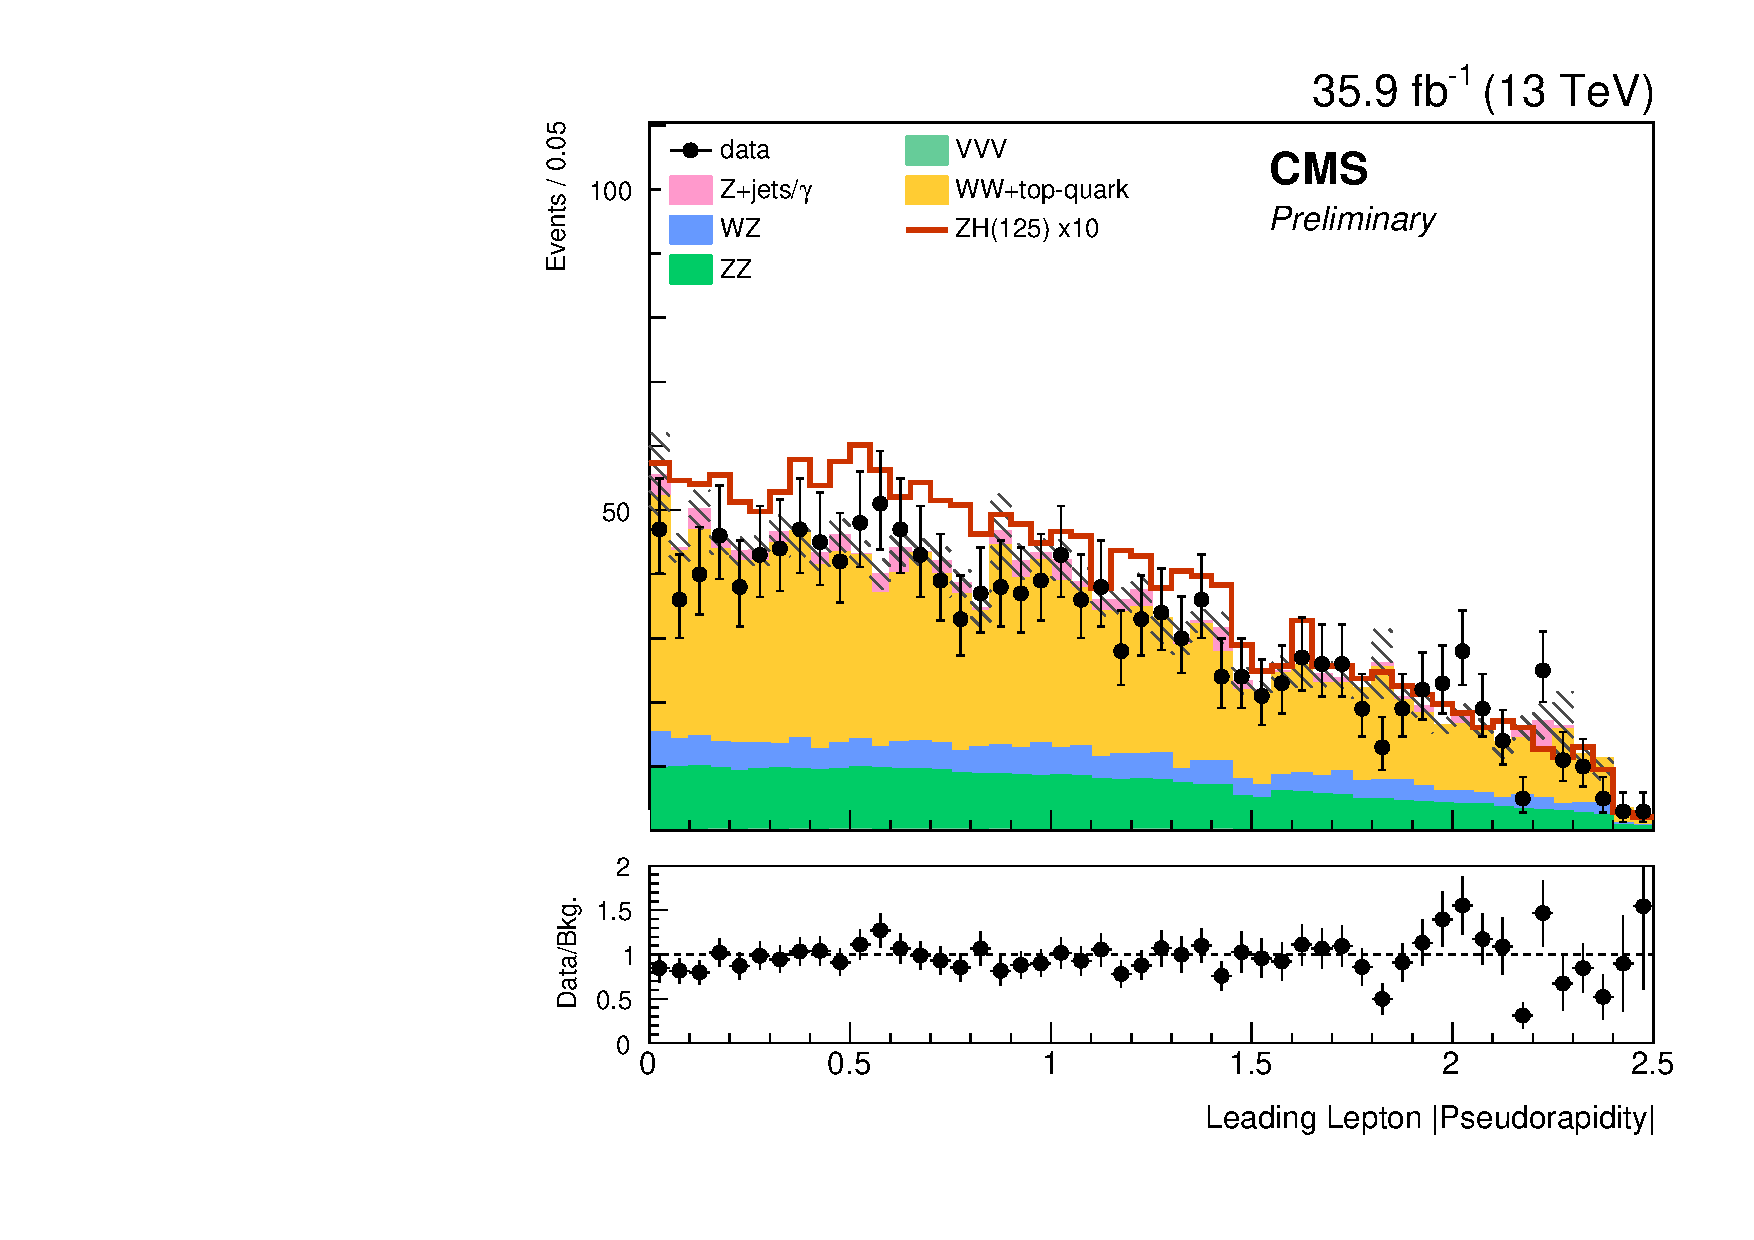
\includegraphics[width=0.48\textwidth]{figures/mva_abs_etal1_nice.pdf}
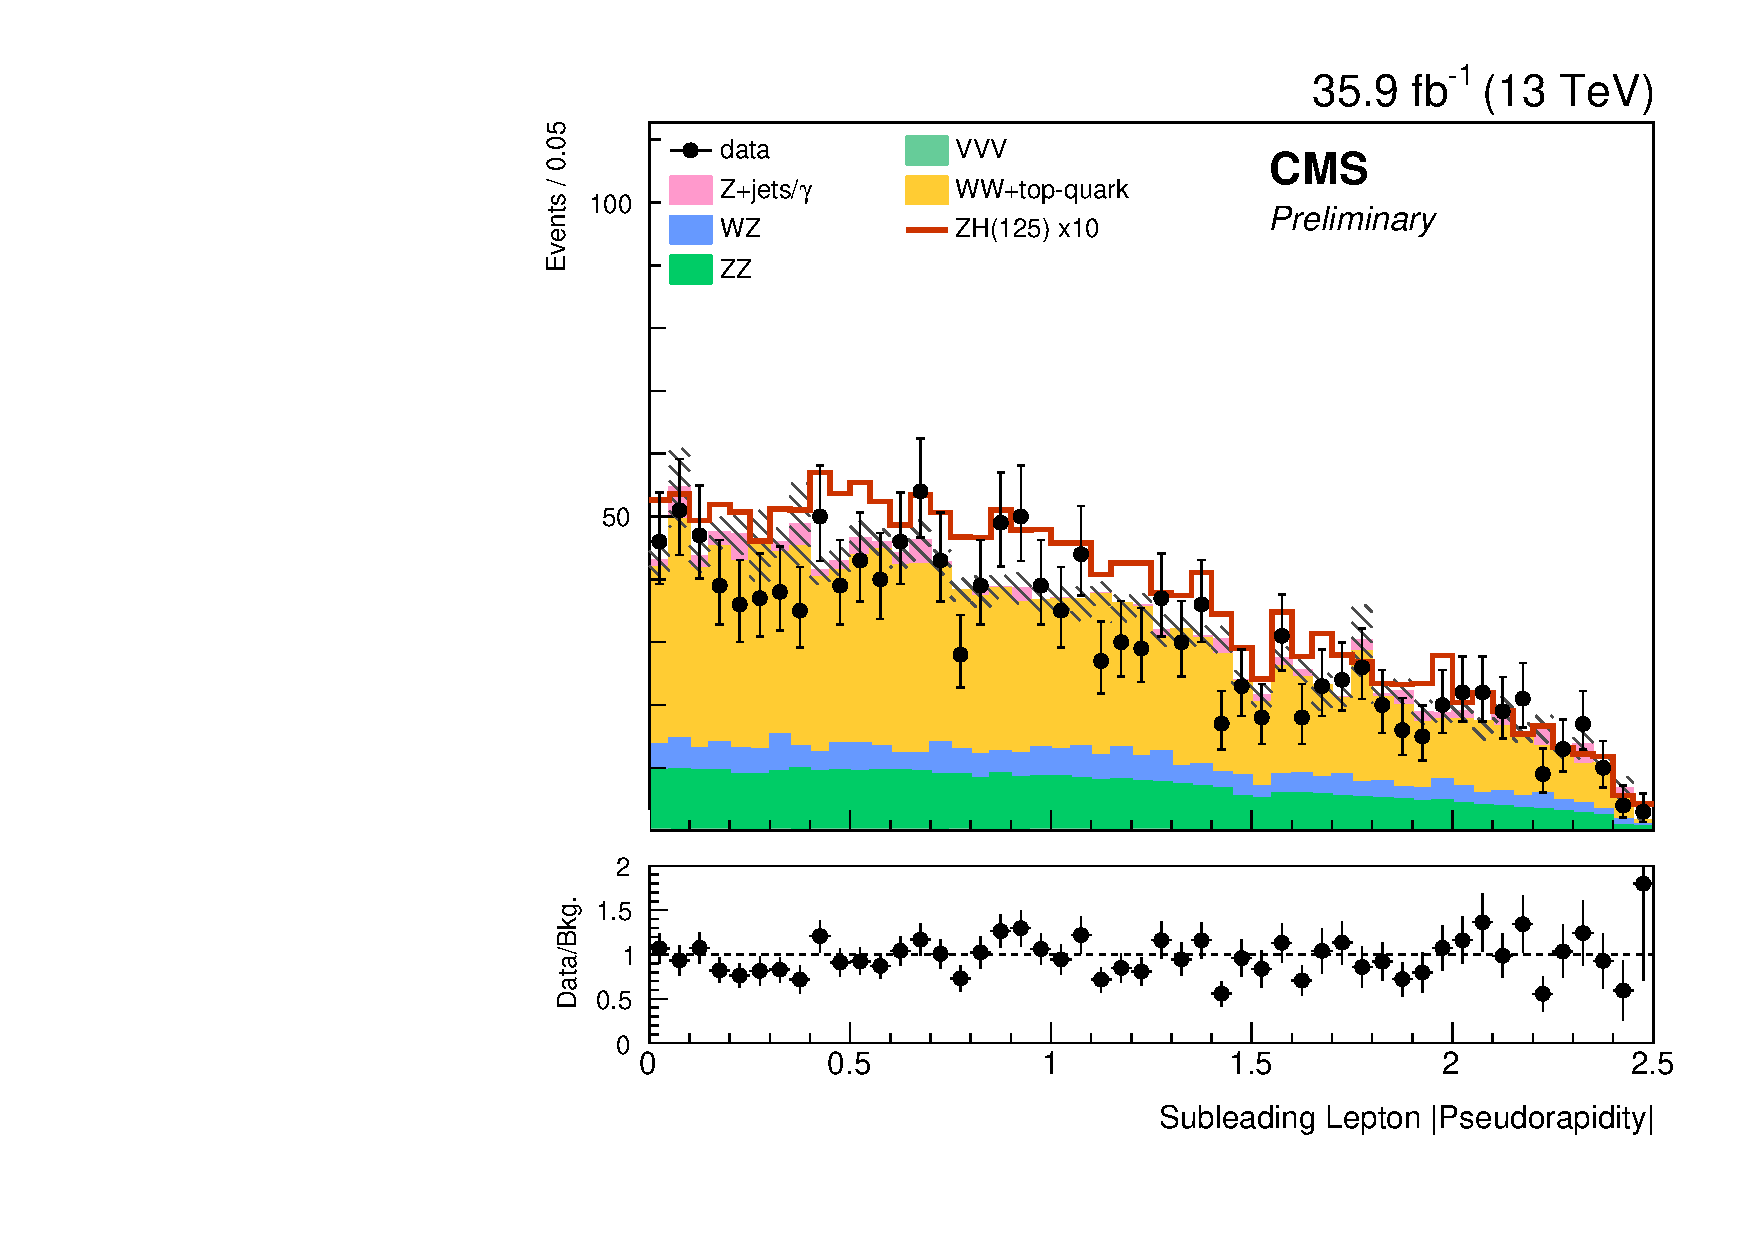
\includegraphics[width=0.48\textwidth]{figures/mva_abs_etal2_nice.pdf}
\caption{(continued, 1) Comparison of data and prediction in the BDT input variables after applying the training preselection. Signal strength has been enhanced by a factor of 10.}
\label{fig:bdt_inputvar_histos2}
\end{center}
\end{figure}

\subsection{Analysis selection} 

The signal region in the multivariate analysis is defined using the training preselection cuts except $\met >$ 100 $\GeV$ and classifier value $>$ 0.2. 
The Drell-Yan normalization is taken from a control selection similar to the rectangular analysis, admitting events which otherwise pass the signal region selectiont with $\met <$ 100 $\GeV$ or classifier value $<$ 0.2.
The non-resonant background normalization is taken from a control sample applying the signal region selection 
described in this section, but requiring opposite-flavor events. The diboson control region 
selections are unchanged from the rectangular analysis. See Figures~\ref{fig:bdt_zh} 
and~\ref{fig:bdt_vv} for the classifier spectrum in the signal region and diboson regions.

The signal hypothesis is considered in a shape analysis of the BDT classifier spectrum. 

\begin{figure}[htbp]
\begin{center}
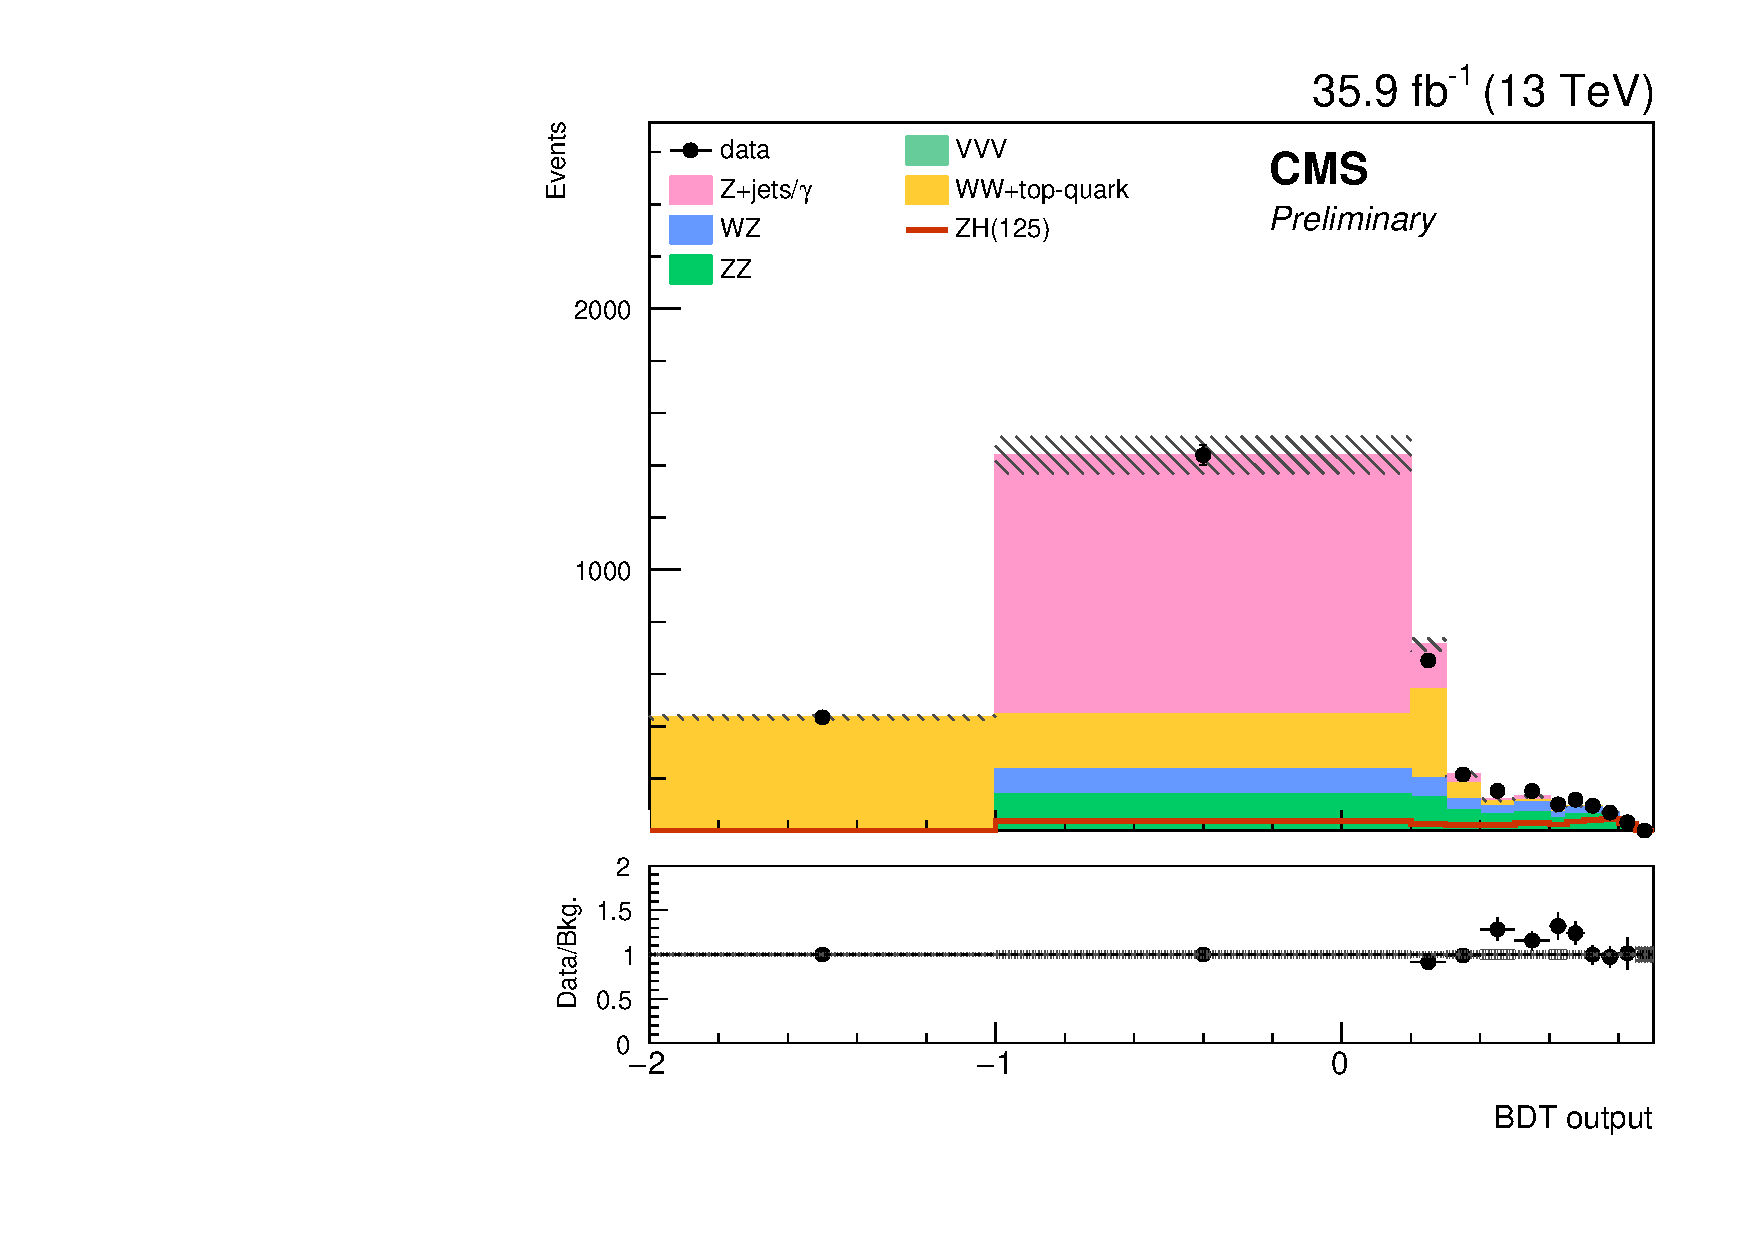
\includegraphics[width=0.48\textwidth]{figures/bdt_zh_prefit.pdf}
\caption{Distribution of the BDT classifier in the multivariate analysis before the likelihood fit. The first bin contains the nonresonant background sideband of opposite-flavor events. The second bin contains the Drell-Yan sideband of events failing the BDT or $\met$ requirement. The rest of the bins are the signal region BDT bins. Uncertainty bands represent only the statistical uncertainty.}
\label{fig:bdt_zh_prefit}
\end{center}
\end{figure}

\begin{figure}[htbp]
\begin{center}
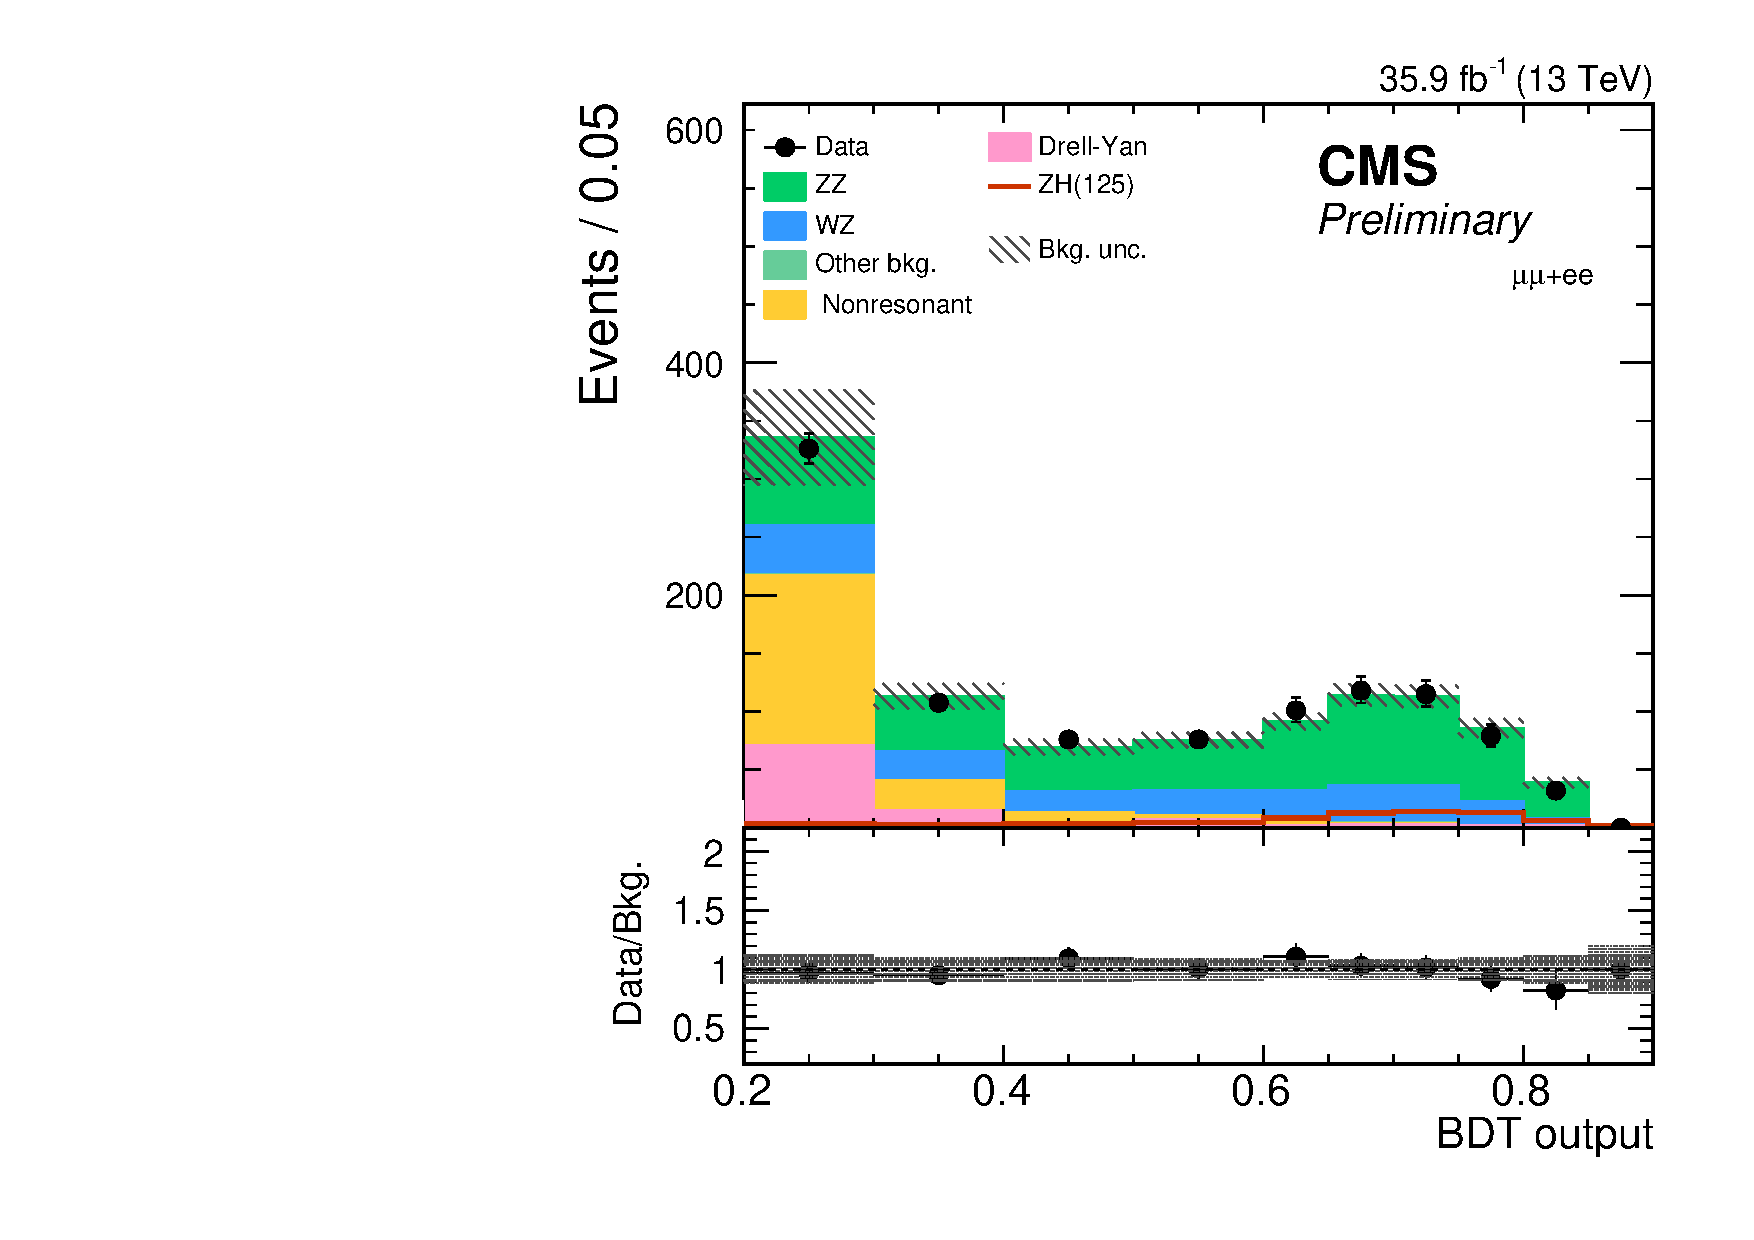
\includegraphics[width=0.48\textwidth]{figures/fullsel_bdt_ll_postfit.pdf}
\caption{Distribution of the BDT classifier in the multivariate analysis signal region after the likelihood fit. Uncertainty bands correspond to both statistical and systematic uncertainty.}
\label{fig:bdt_zh}
\end{center}
\end{figure}

\begin{figure}[htbp]
\begin{center}
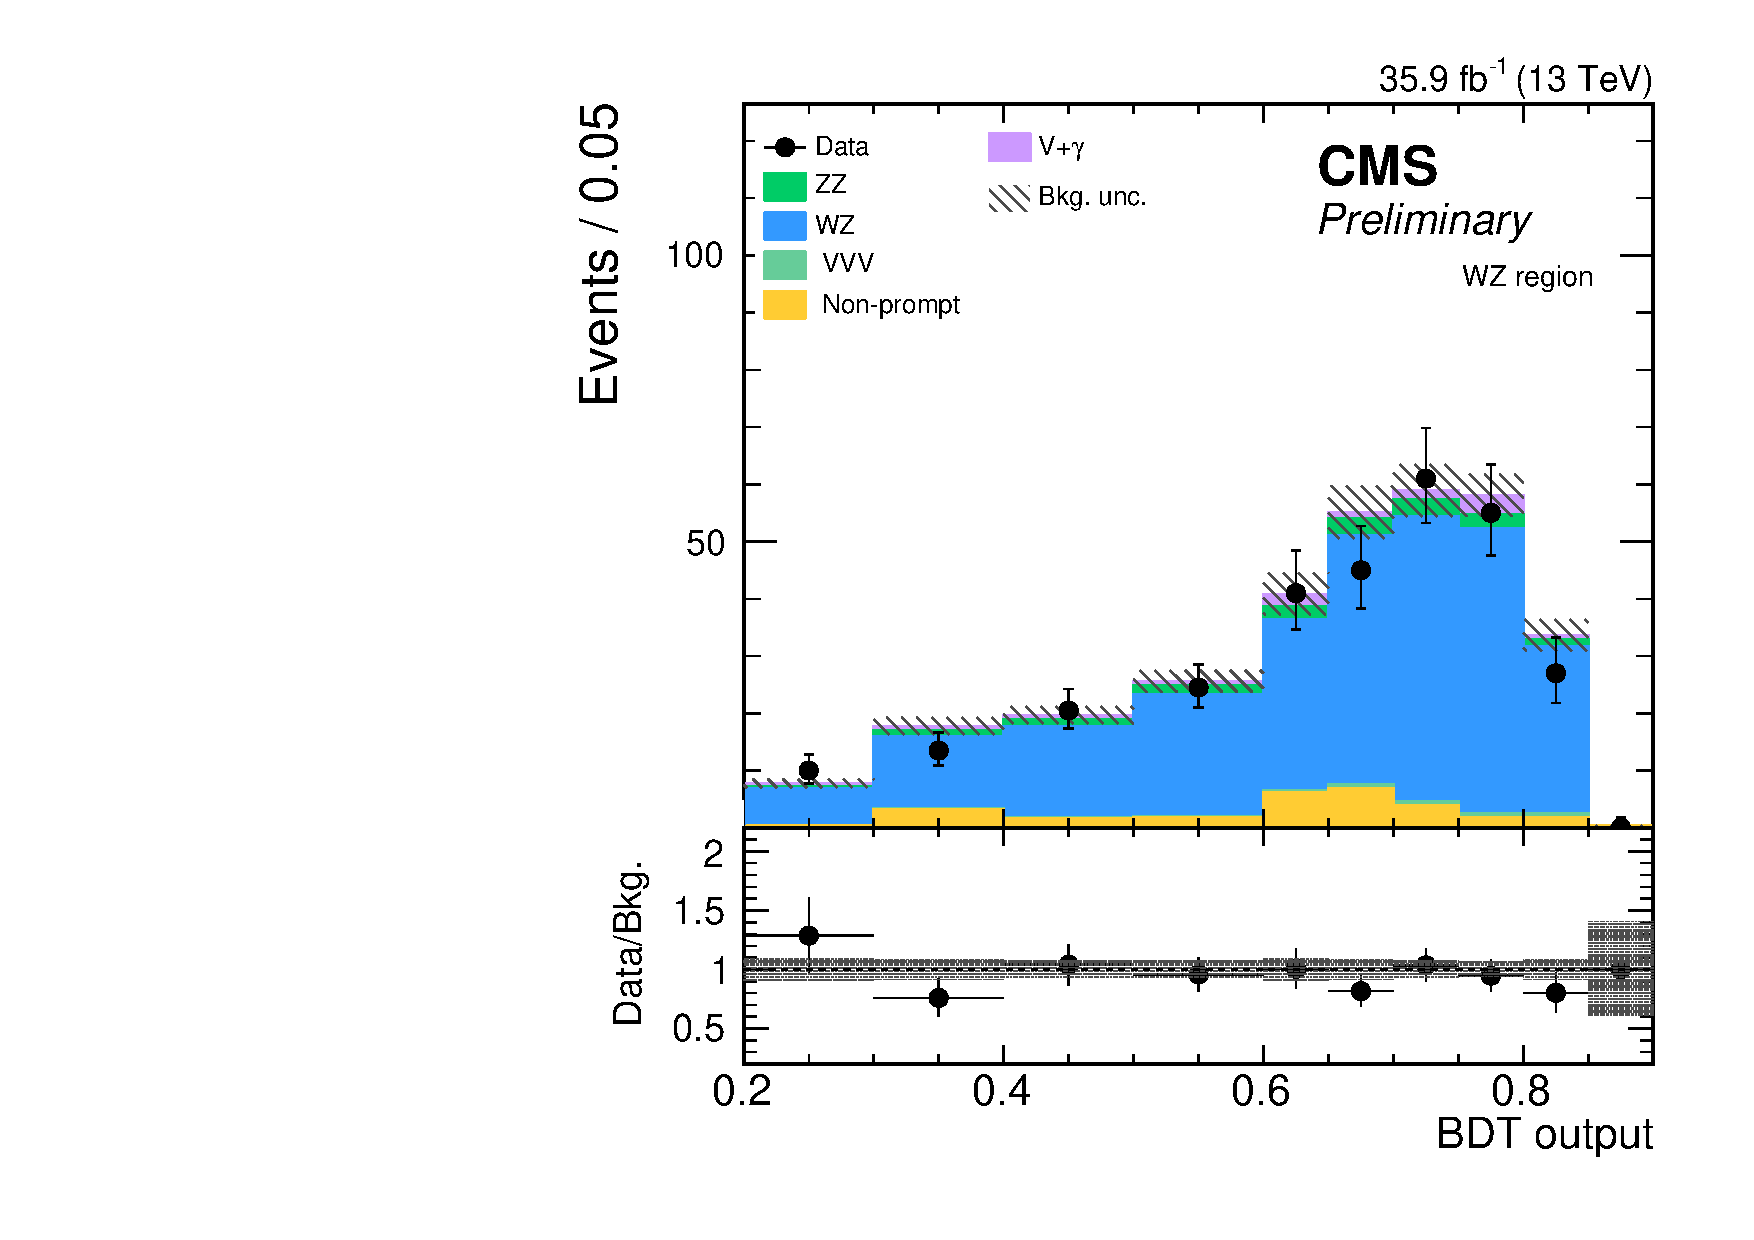
\includegraphics[width=0.48\textwidth]{figures/fullsel_bdt_wz_postfit.pdf}
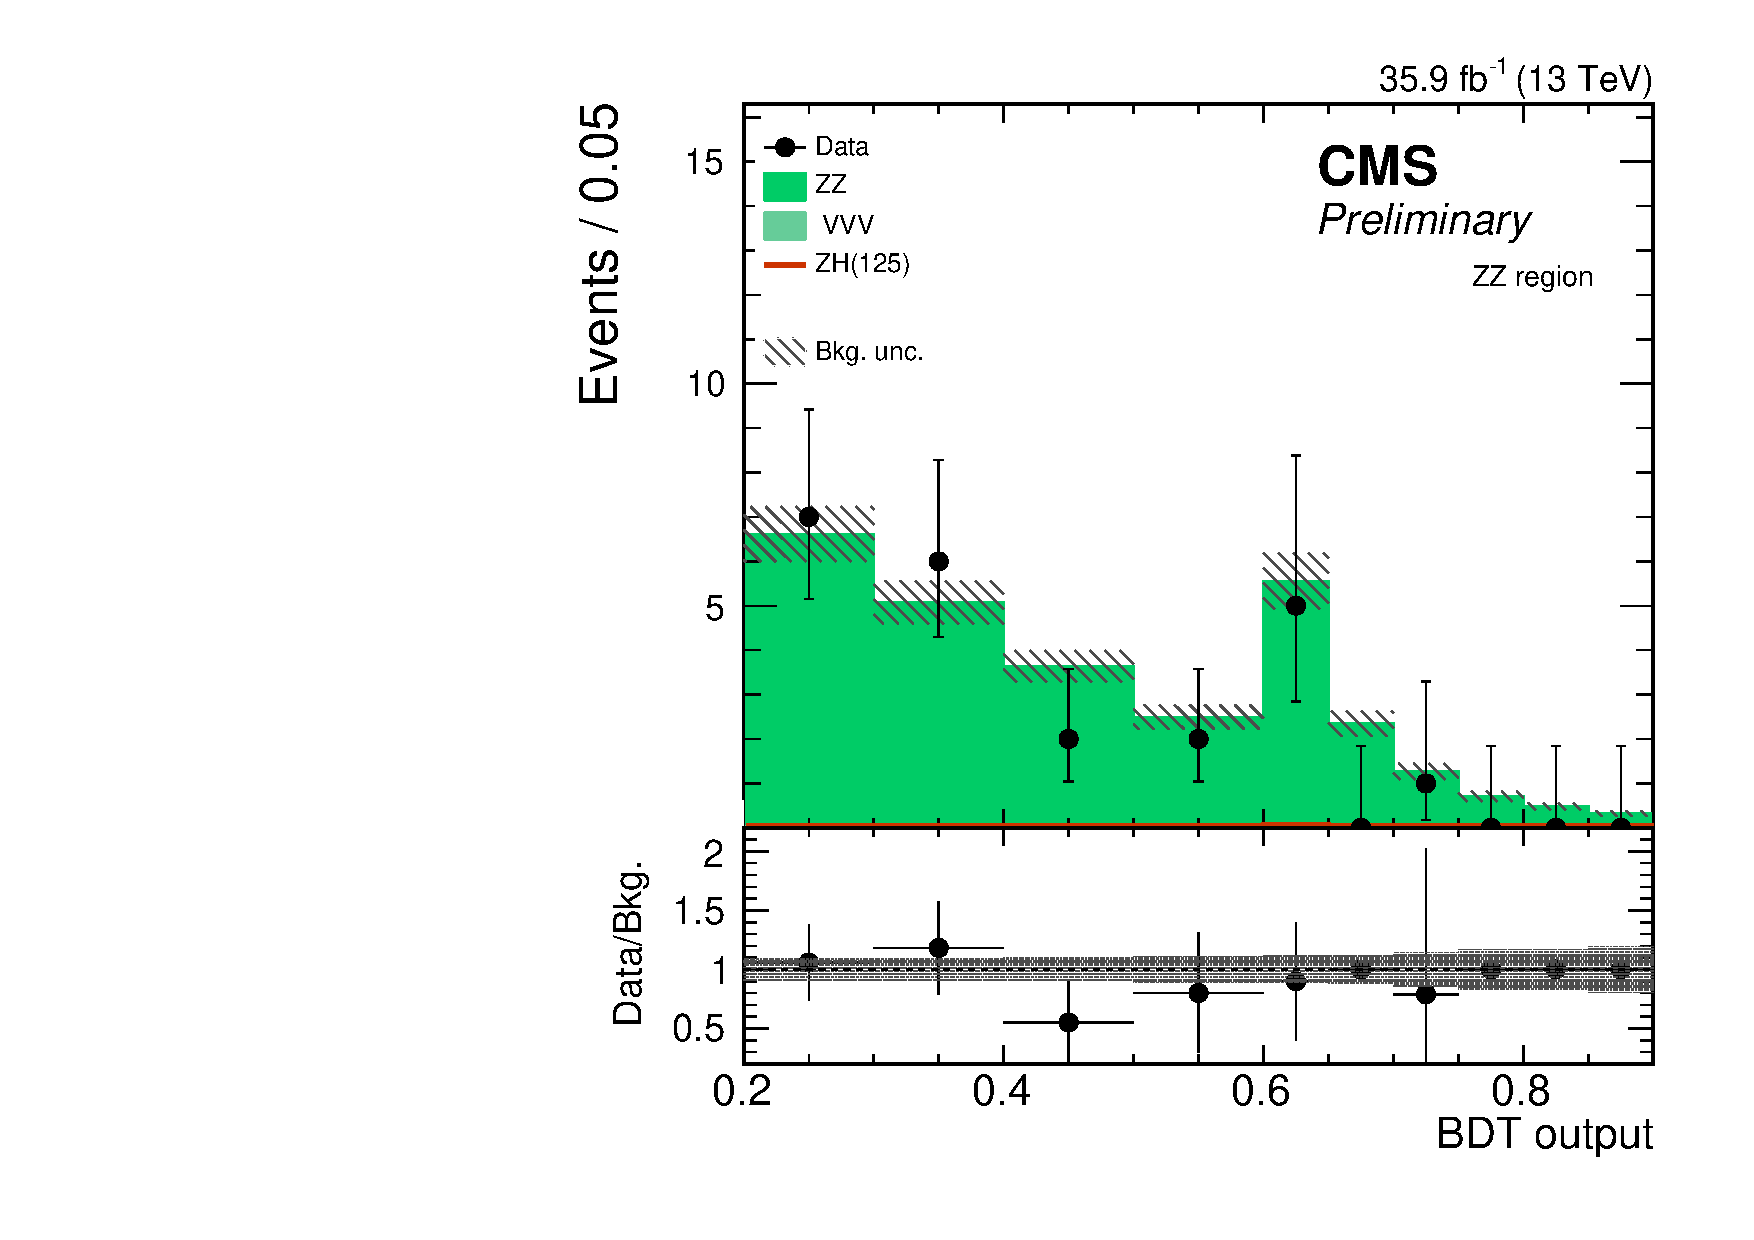
\includegraphics[width=0.48\textwidth]{figures/fullsel_bdt_zz_postfit.pdf}
\caption{Distribution of the BDT classifier in the diboson control regions: WZ three-lepton region at left, ZZ four-lepton region at right. Uncertainty bands correspond to both statistical and systematic uncertainty.}
\label{fig:bdt_vv}
\end{center}
\end{figure}
\clearpage
\subsection{Propagation of uncertainties} 
In order to perform a shape analysis in the classifier BDT spectrum, the effect of various nuisance parameters must be propagated to the BDT shape.
It is not sufficient to simply evaluate different shapes at the extremities of the nuisance variations, because a BDT is not a conformal map.
Therefore, we used a toy method to sample the distributions of the relevant nuisance parameters and found the resulting distributions in BDT value.
The nuisances considered to be relevant are the lepton scale uncertainties and the uncertainty in missing energy due to the jet energy scale.

The number of random toys used for the uncertainty propagation was 50 due to the high computing cost of many classifier evaluations. 
The lepton scale variations were sampled from a normal distribution with standard deviation of 0.01.
The \met variations were sampled from a normal distribution with standard deviation of 1, then multiplied by the relative size of the jet energy scale effect (this quantity varies per event).
Variations in the lepton scale affected the missing energy which was adjusted; variations in the missing energy affected many of the other variables, which were subsequently adjusted. 

After performing this procedure for all simulated events, we take the uncertainty bands from the non-normal toy distributions as the distance between the 15.9\% and 84.1\% quantiles.
Figures~\ref{fig:bdt_toy_envelopes_electron},~\ref{fig:bdt_toy_envelopes_muon}, and~\ref{fig:bdt_toy_envelopes_MET} show 2D maps of the nuisance variations with the BDT value on the horizontal axis and the relative variation from the nominal BDT bin yield on the vertical axis.
Figures~\ref{fig:bdt_electron_scale},~\ref{fig:bdt_muon_scale}, and~\ref{fig:bdt_MET_scale} show the resulting uncertainty shapes that enter the likelihood fit, for the electron scale, muon scale, and MET scale nuisances respectively. 
In most combinations of background process and nuisance parameter, the propagated uncertainty is irrelevant compared to the statistical uncertainty from the number of simulated events.

We do not propagate this uncertainty for the non-resonant backgrounds or the Drell-Yan process, since they are not highly signal like and the other extrapolation uncertainties are sufficiently conservative.
Furthermore, when performing the likelihood fit to determine the exclusion limits, we ignore these propagated uncertainties in the ratio of the diboson control regions, and fully correlate them across the shape bins in the signal region. 

\begin{figure}[htbp]
\begin{center}
\includegraphics[width=0.48\textwidth]{figures/syst_BDT_ZH_hinv_sm_toyenvelope_electron.pdf}
\includegraphics[width=0.48\textwidth]{figures/syst_BDT_ggZH_hinv_toyenvelope_electron.pdf}
\includegraphics[width=0.48\textwidth]{figures/syst_BDT_ZZ_toyenvelope_electron.pdf}
\includegraphics[width=0.48\textwidth]{figures/syst_BDT_WZ_toyenvelope_electron.pdf}
\includegraphics[width=0.48\textwidth]{figures/syst_BDT_VVV_toyenvelope_electron.pdf}
\caption{2D maps of the relative toy variations from the nominal BDT shape versus the BDT value, for the electron scale. The hashed bands represent statistical uncertainty on the simulated events.}
\label{fig:bdt_toy_envelopes_electron}
\end{center}
\end{figure}

\begin{figure}[htbp]
\begin{center}
\includegraphics[width=0.48\textwidth]{figures/syst_BDT_ZH_hinv_sm_toyenvelope_muon.pdf}
\includegraphics[width=0.48\textwidth]{figures/syst_BDT_ggZH_hinv_toyenvelope_muon.pdf}
\includegraphics[width=0.48\textwidth]{figures/syst_BDT_ZZ_toyenvelope_muon.pdf}
\includegraphics[width=0.48\textwidth]{figures/syst_BDT_WZ_toyenvelope_muon.pdf}
\includegraphics[width=0.48\textwidth]{figures/syst_BDT_VVV_toyenvelope_muon.pdf}
\caption{2D maps of the relative toy variations from the nominal BDT shape versus the BDT value, for the muon scale. The hashed bands represent statistical uncertainty on the simulated events.}
\label{fig:bdt_toy_envelopes_muon}
\end{center}
\end{figure}

\begin{figure}[htbp]
\begin{center}
\includegraphics[width=0.48\textwidth]{figures/syst_BDT_ZH_hinv_sm_toyenvelope_MET.pdf}
\includegraphics[width=0.48\textwidth]{figures/syst_BDT_ggZH_hinv_toyenvelope_MET.pdf}
\includegraphics[width=0.48\textwidth]{figures/syst_BDT_ZZ_toyenvelope_MET.pdf}
\includegraphics[width=0.48\textwidth]{figures/syst_BDT_WZ_toyenvelope_MET.pdf}
\includegraphics[width=0.48\textwidth]{figures/syst_BDT_VVV_toyenvelope_MET.pdf}
\caption{2D maps of the relative toy variations from the nominal BDT shape versus the BDT value, for the \met scale due to the JES uncertainty. The hashed bands represent statistical uncertainty on the simulated events.}
\label{fig:bdt_toy_envelopes_MET}
\end{center}
\end{figure}

\begin{figure}[htbp]
\begin{center}
\includegraphics[width=0.48\textwidth]{figures/syst_BDT_ZH_hinv_sm_toys_electron.pdf}
\includegraphics[width=0.48\textwidth]{figures/syst_BDT_ggZH_hinv_toys_electron.pdf}
\includegraphics[width=0.48\textwidth]{figures/syst_BDT_ZZ_toys_electron.pdf}
\includegraphics[width=0.48\textwidth]{figures/syst_BDT_WZ_toys_electron.pdf}
\includegraphics[width=0.48\textwidth]{figures/syst_BDT_VVV_toys_electron.pdf}
\caption{Uncertainty shapes calculated from the toy method for the electron scale.}
\label{fig:bdt_electron_scale}
\end{center}
\end{figure}

\begin{figure}[htbp]
\begin{center}
\includegraphics[width=0.48\textwidth]{figures/syst_BDT_ZH_hinv_sm_toys_muon.pdf}
\includegraphics[width=0.48\textwidth]{figures/syst_BDT_ggZH_hinv_toys_muon.pdf}
\includegraphics[width=0.48\textwidth]{figures/syst_BDT_ZZ_toys_muon.pdf}
\includegraphics[width=0.48\textwidth]{figures/syst_BDT_WZ_toys_muon.pdf}
\includegraphics[width=0.48\textwidth]{figures/syst_BDT_VVV_toys_muon.pdf}
\caption{Uncertainty shapes calculated from the toy method for the muon scale.}
\label{fig:bdt_muon_scale}
\end{center}
\end{figure}

\begin{figure}[htbp]
\begin{center}
\includegraphics[width=0.48\textwidth]{figures/syst_BDT_ZH_hinv_sm_toys_MET.pdf}
\includegraphics[width=0.48\textwidth]{figures/syst_BDT_ggZH_hinv_toys_MET.pdf}
\includegraphics[width=0.48\textwidth]{figures/syst_BDT_ZZ_toys_MET.pdf}
\includegraphics[width=0.48\textwidth]{figures/syst_BDT_WZ_toys_MET.pdf}
\includegraphics[width=0.48\textwidth]{figures/syst_BDT_VVV_toys_MET.pdf}
\caption{Uncertainty shapes calculated from the toy method for the \met due to the JES uncertainty.}
\label{fig:bdt_MET_scale}
\end{center}
\end{figure}


\subsection{Improvement in sensitivity} 
The BDT analysis improves the invisible Higgs(125) sensitivity by 10\%.
Taking this approach is not nearly as rewarding for the higher mass simplified-model DM signals, where \met is a more powerful discriminant variable.
These cases require further study before multivariate techniques can be exploited there.

\section{Search results}
